\section{面向基于主动丢包的VoLTE时间隐通道检测方法评估}
\label{chap:analyze:result}

%本节讲述的内容,对提出的测试方法,进行检验
在\nref{chap:analyze:statistical}中,提出了针对VoLTE下主动丢包时间隐通道的检测方法,本节以实验验证的方式,对该检测方法的检测能力进行评估。基于抓包得到的测试样本,通过随机丢包的方式模拟时间隐通道的行为,使用检测方法判断是否存在隐通道,评估检测准确度。

\subsection{评估方法概述}
\label{chap:analyze:result:abstract}

%测试的数据集
用于测试的数据集,来自VoLTE视频通话中,对视频数据包的抓包结果。如表\nref{tab:3:capture-results}所示,抓包结果分为两种场景,在测试中也按照场景的划分独立进行。

%如何模拟测试(随机丢包)、参数
基于主动丢包的时间隐通道,通常产生一定比例的随机丢包,并且具有相对稳定的随机丢包率。在验证过程中,设定了10\%、5\%、2\%、1\%、0.4\%、0.2\%及0.1\%几种不同的丢包比例,在区间中随机选择丢包对象。

%统计结果进行测试
根据检测方法的设计,判断过程为全参照的双样本检测,在评估过程中,选择宿主信道的分布为参照样本,选择时间隐通道的分布为检测样本。最终根据通过项数进行判断。

\subsection{IPD测试结果评估}
\label{chap:analyze:result:ipd}

本节介绍的是对IPD分布的测试,在测试样本中,IPD数据量较大,因此对时间隐通道的存在比较敏感。按照对IPD的检测方式,分别进行测试,并最终汇总对IPD分布检测的结论。

\insertFigure{
	\begin{figure}
        \centering
        \subfigure[Excellent场景的CDF]{
            \label{fig:3:result:ipd:cdf:excellent}
            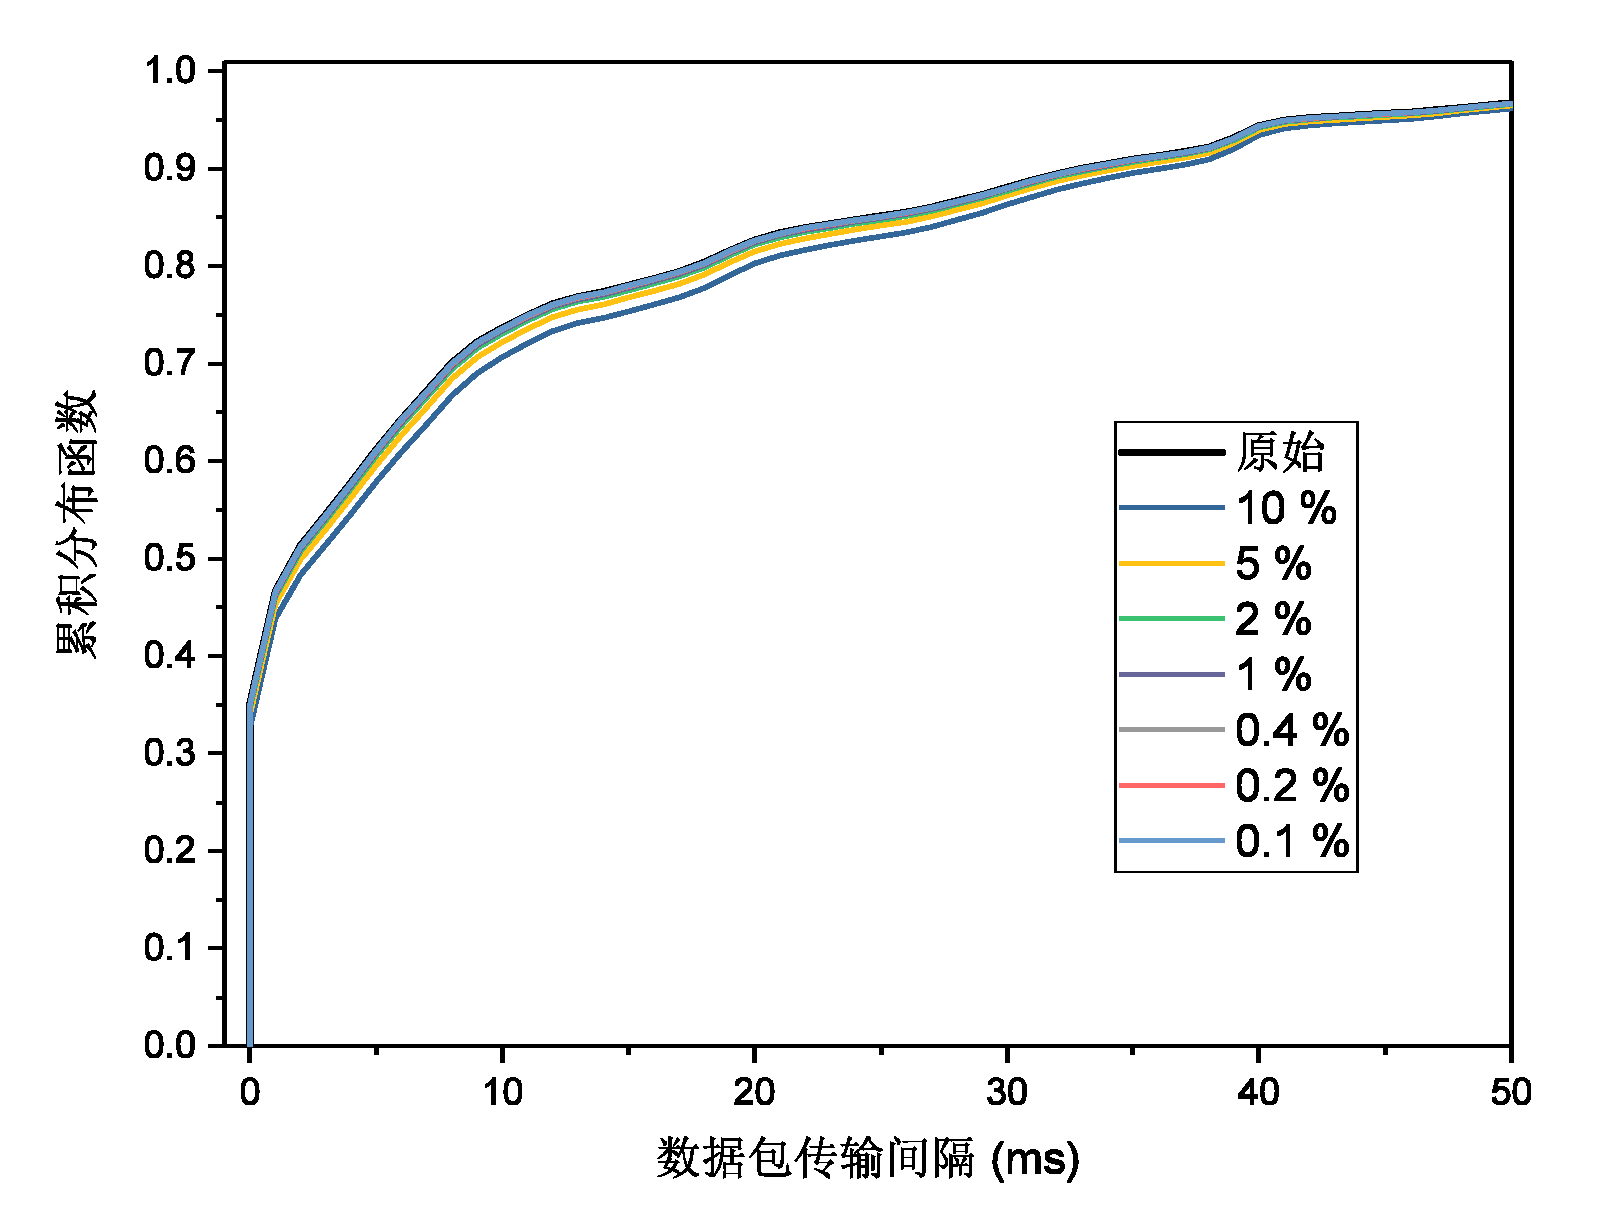
\includegraphics[width=0.48\textwidth]{chapters/chapter3/figures/ipd-cdf-excellent.pdf}
        }
        \subfigure[Good场景的CDF]{
            \label{fig:3:result:ipd:cdf:good}
            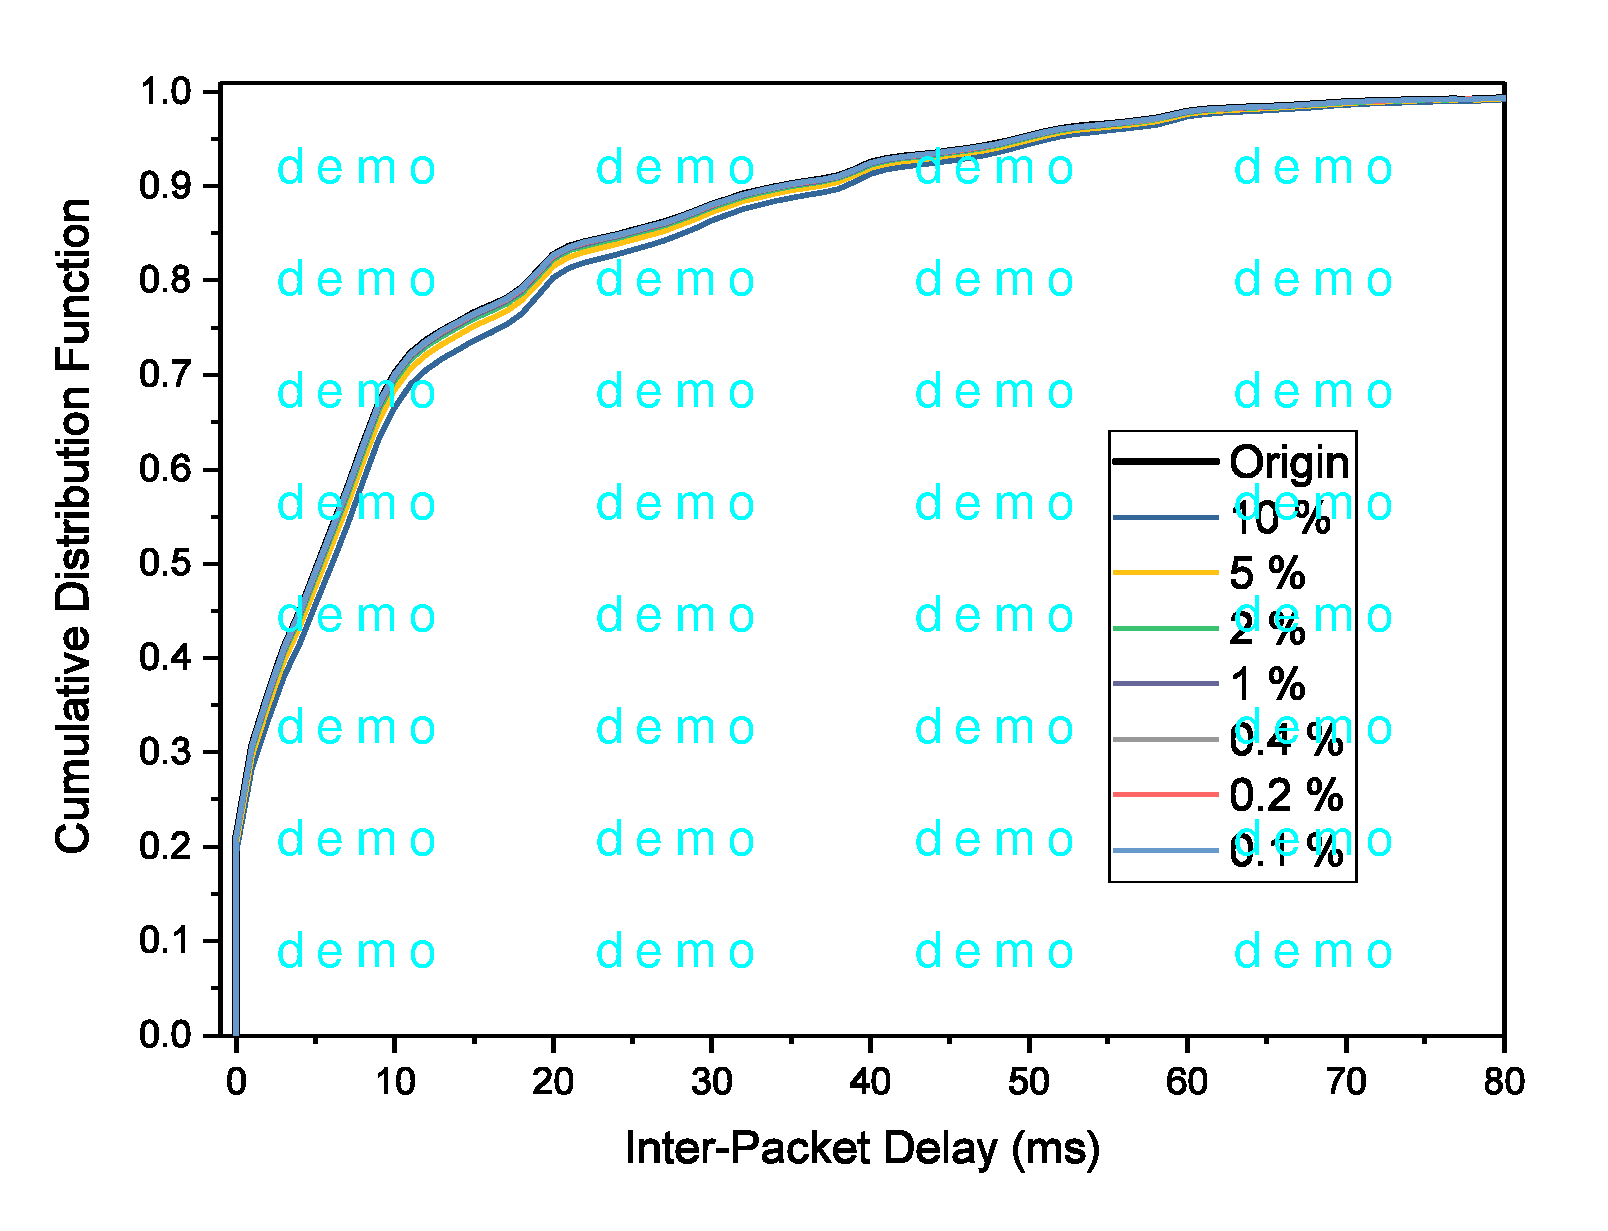
\includegraphics[width=0.48\textwidth]{chapters/chapter3/figures/ipd-cdf-good.pdf}
        }
        \caption{IPD分布的CDF曲线}
        \label{fig:3:result:ipd:cdf}
	\end{figure}
}

\insertFigure{
	\begin{figure}
        \centering
        \subfigure[Excellent场景的箱线图]{
            \label{fig:3:result:ipd:kld:excellent}
            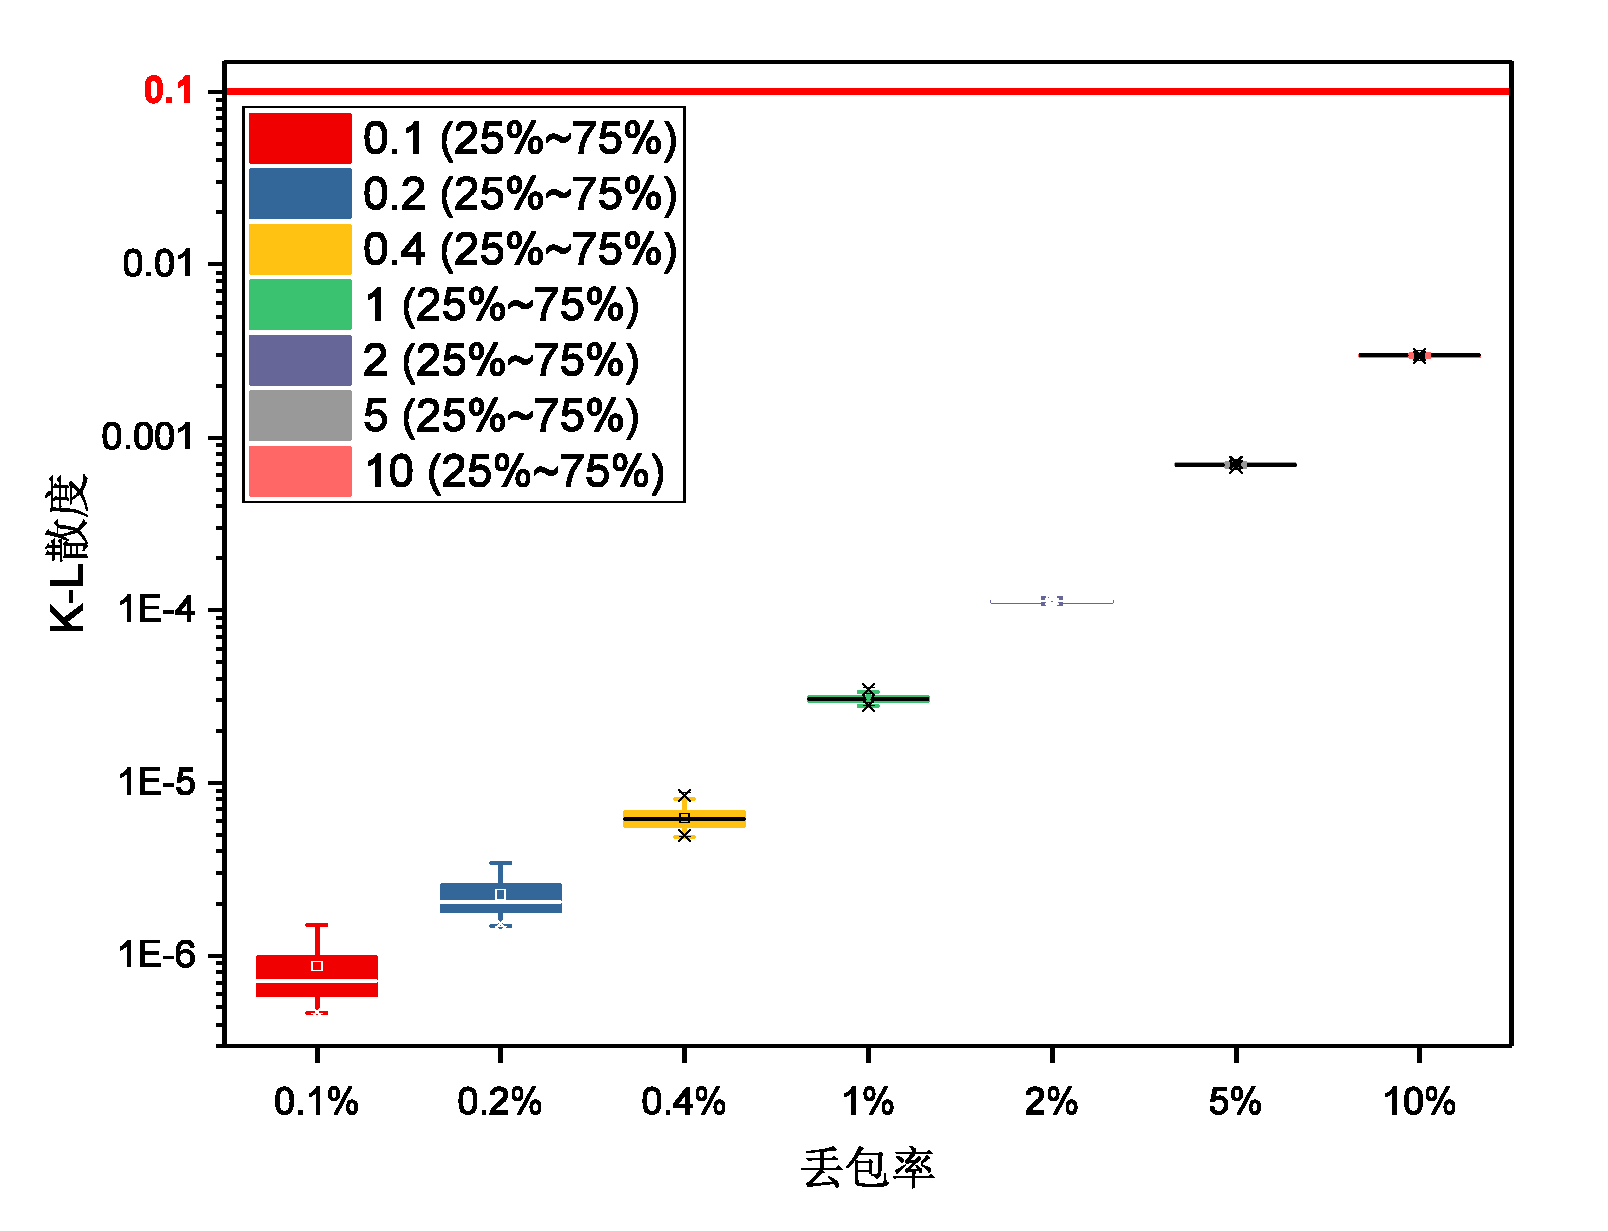
\includegraphics[width=0.48\textwidth]{chapters/chapter3/figures/ipd-kld-excellent.pdf}
        }
        \subfigure[Good场景的箱线图]{
            \label{fig:3:result:ipd:kld:good}
            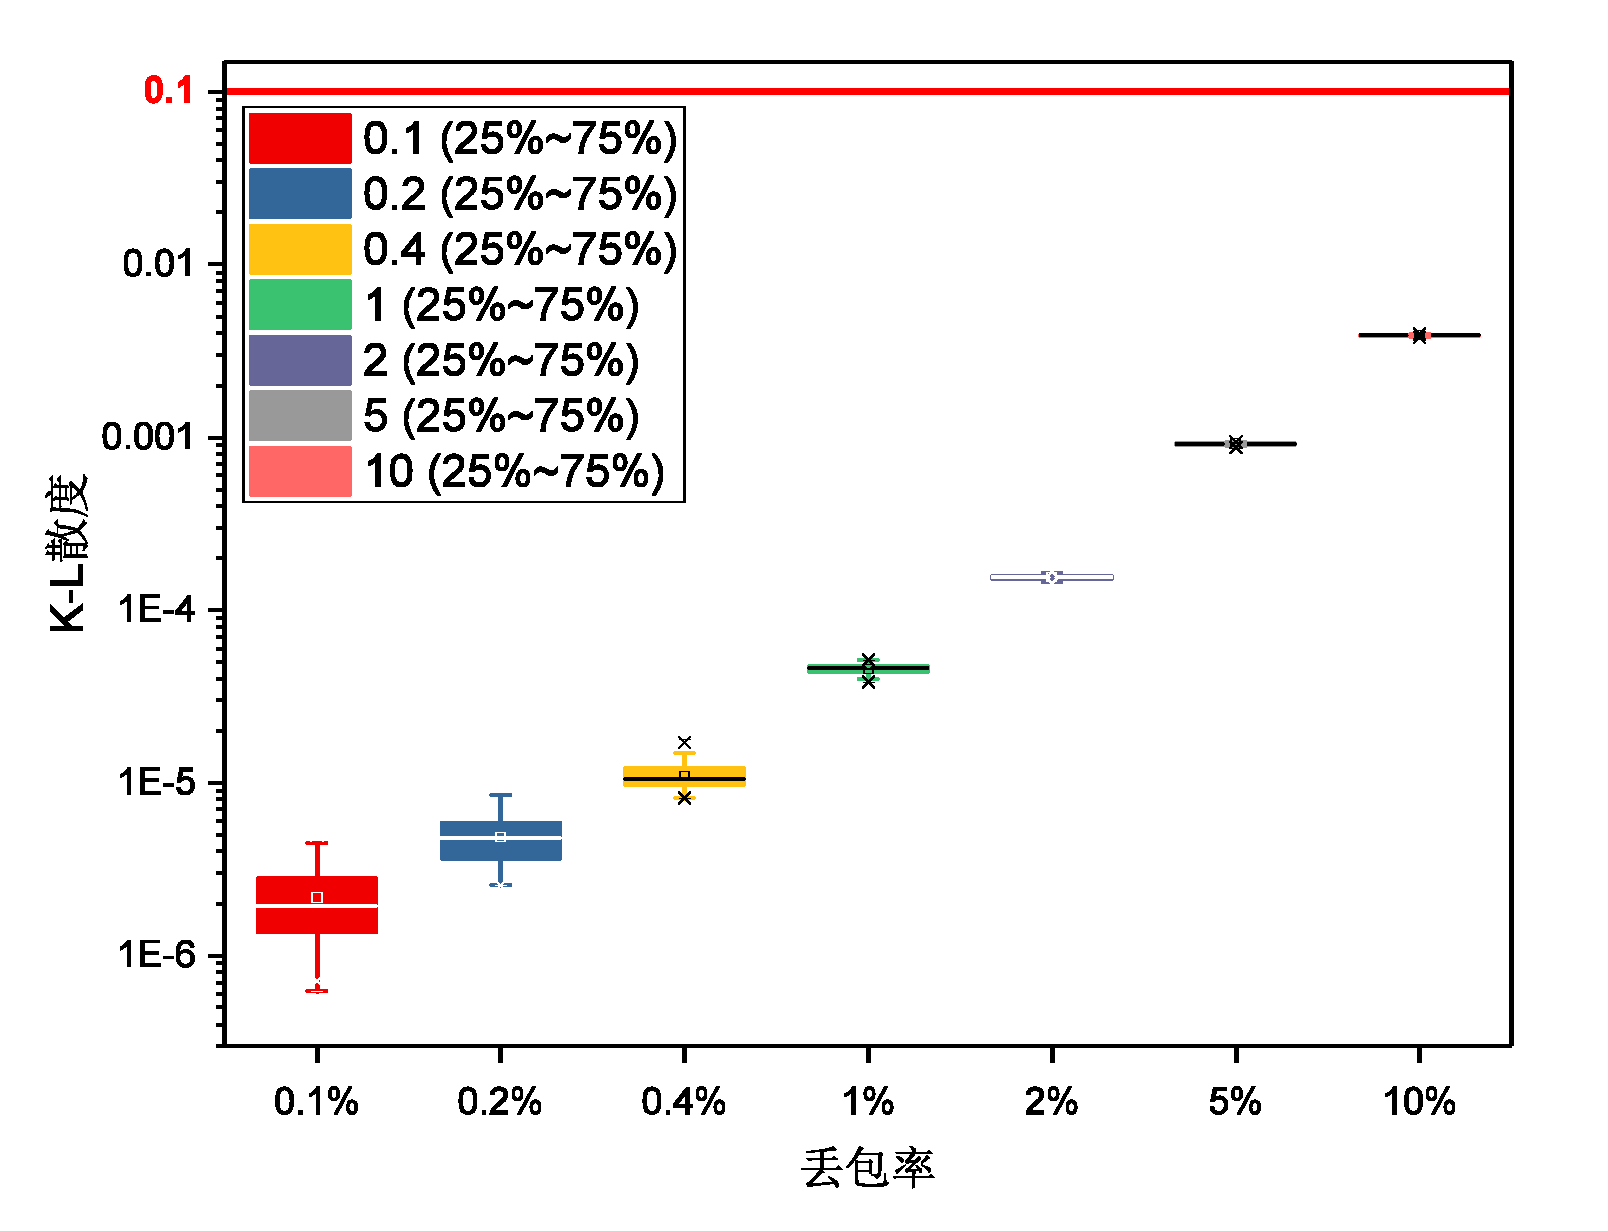
\includegraphics[width=0.48\textwidth]{chapters/chapter3/figures/ipd-kld-good.pdf}
        }
        \caption{IPD分布K-L散度测试结果的箱线图}
        \label{fig:3:result:ipd:kld}
	\end{figure}
}

\insertFigure{
	\begin{figure}
        \centering
        \subfigure[Excellent场景p值的箱线图]{
            \label{fig:3:result:ipd:ks:excellent}
            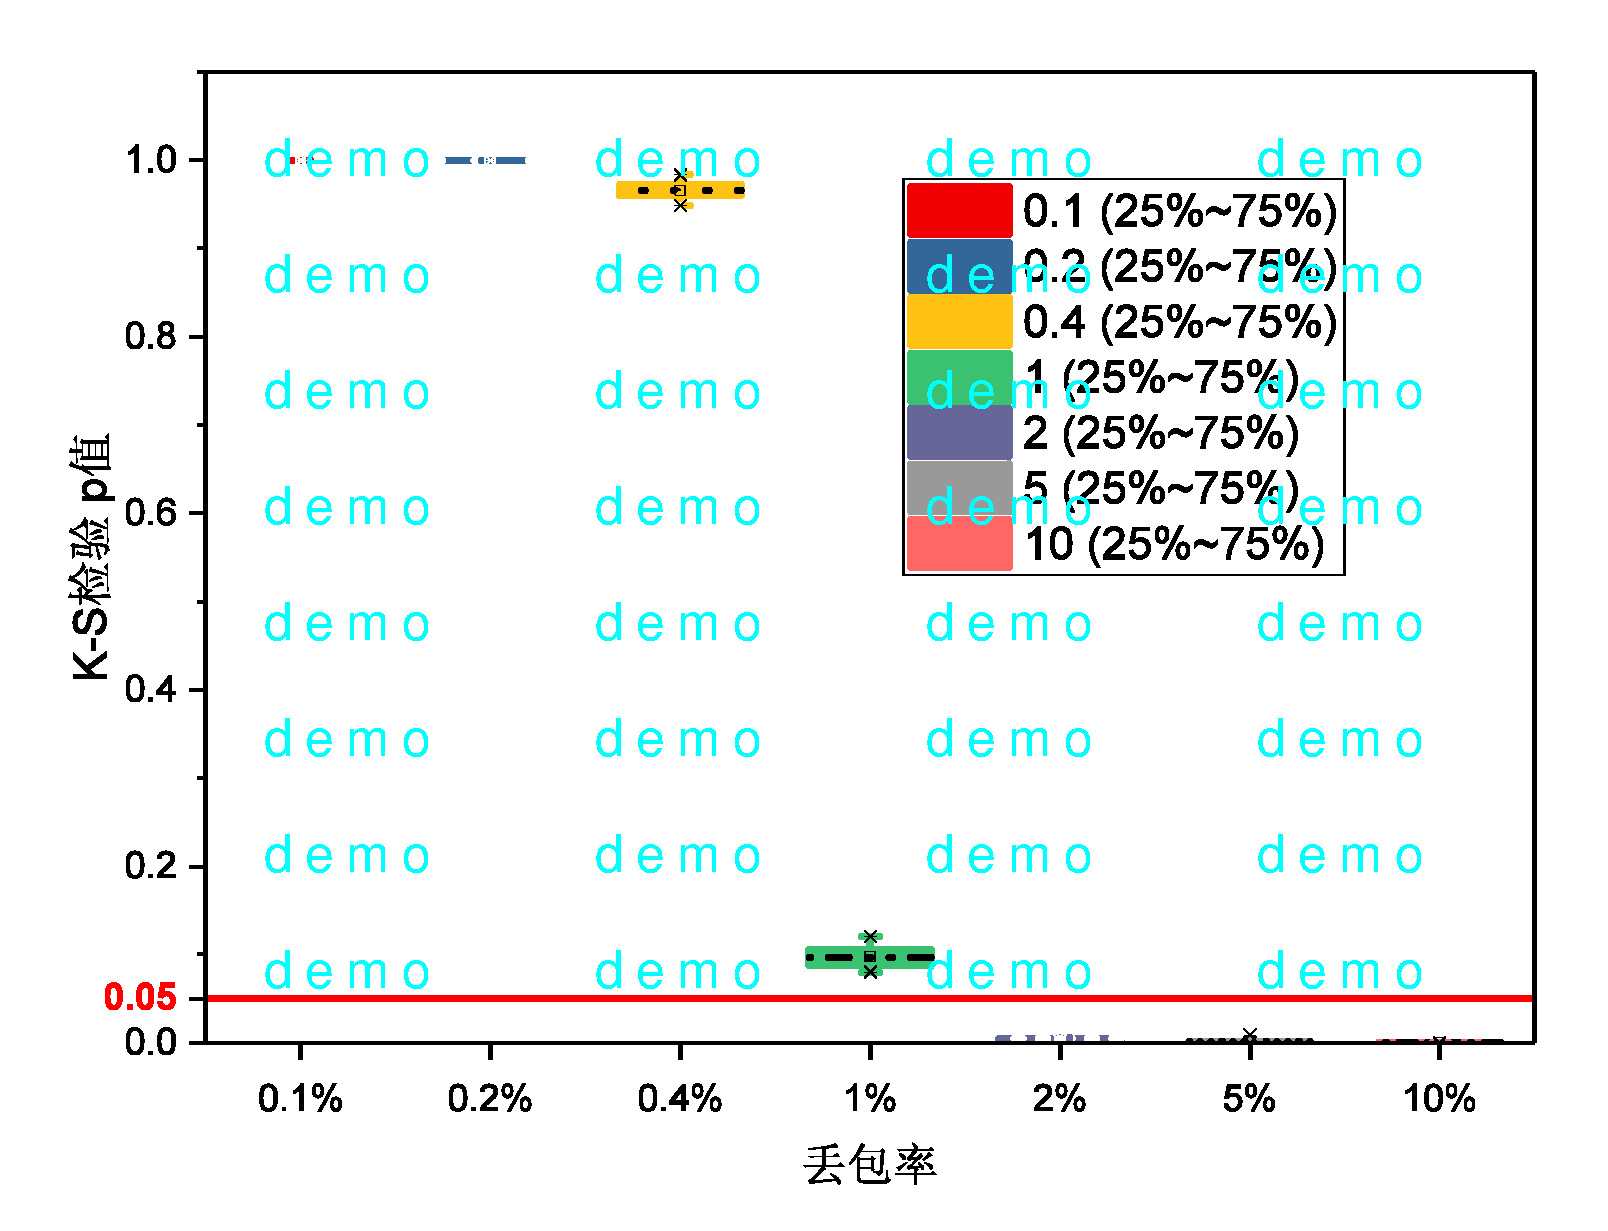
\includegraphics[width=0.48\textwidth]{chapters/chapter3/figures/ipd-ks-excellent.pdf}
        }
        \subfigure[Good场景p值的箱线图]{
            \label{fig:3:result:ipd:ks:good}
            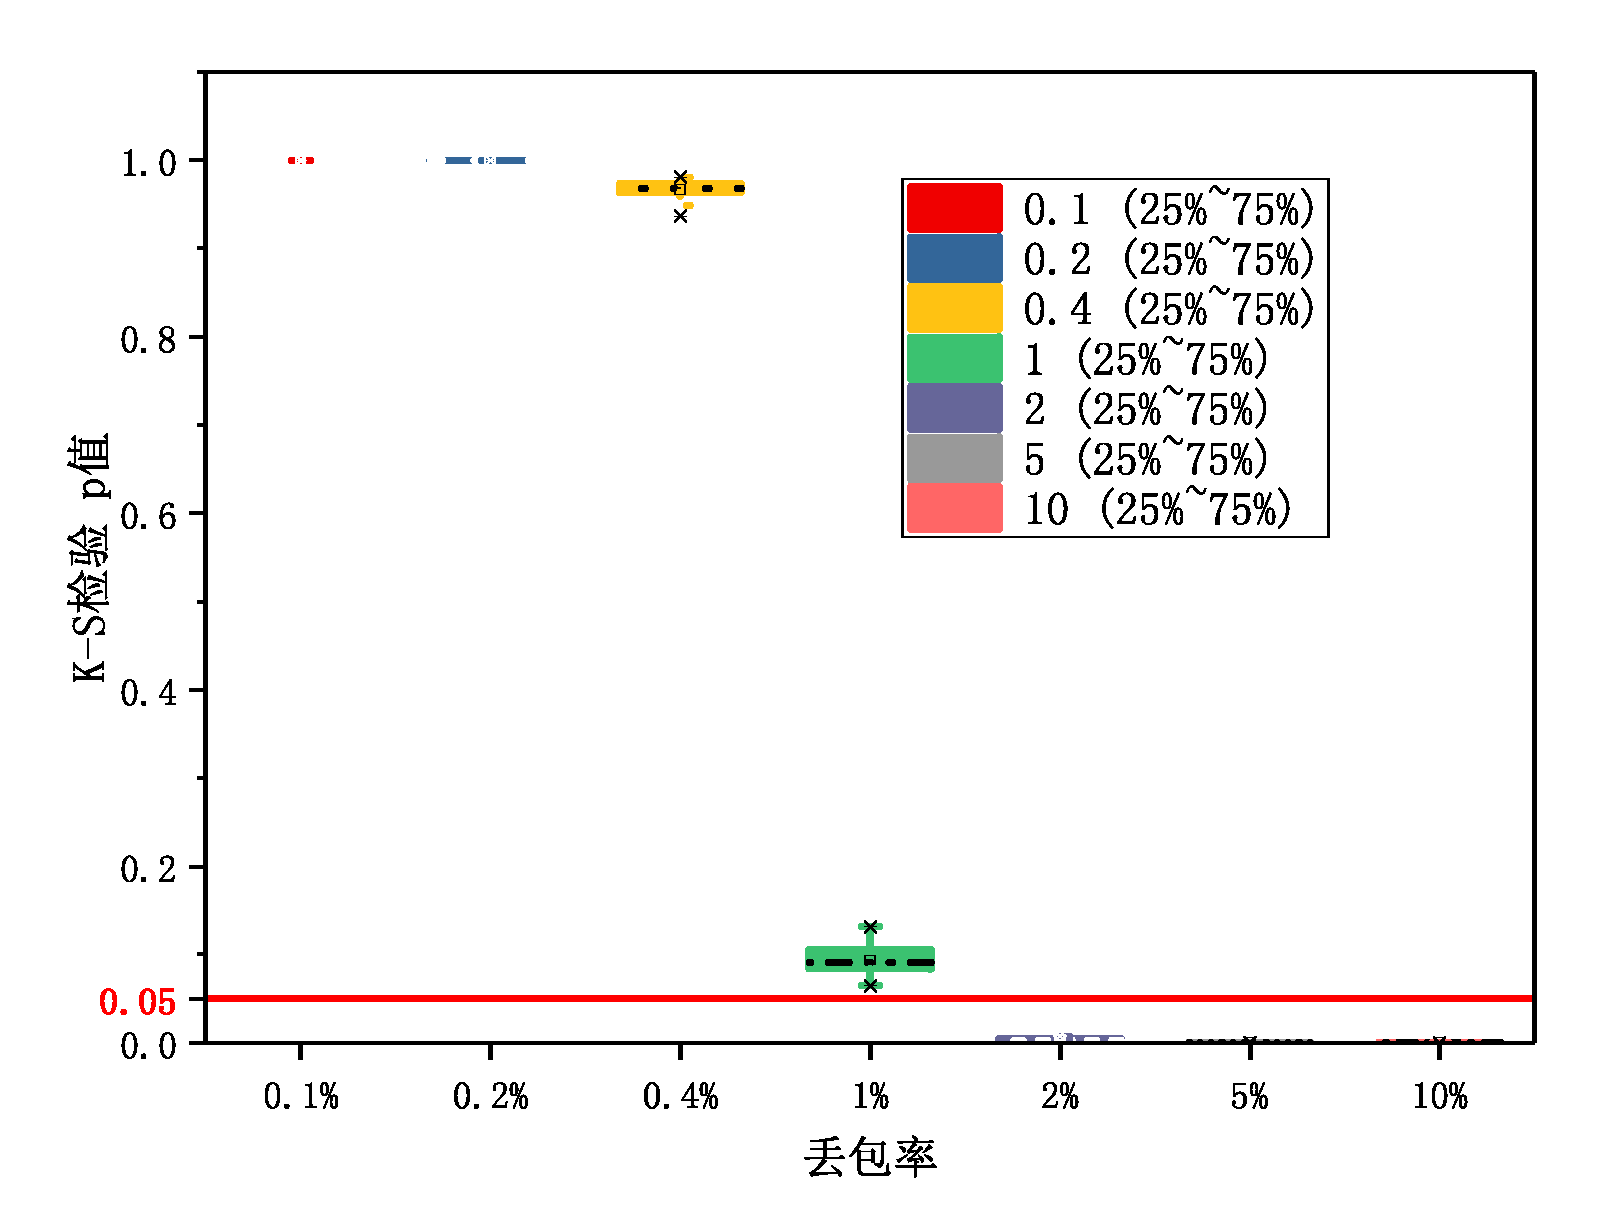
\includegraphics[width=0.48\textwidth]{chapters/chapter3/figures/ipd-ks-good.pdf}
        }
        \caption{IPD分布K-S检验结果的箱线图}
        \label{fig:3:result:ipd:ks}
	\end{figure}
}

\insertFigure{
	\begin{figure}
        \centering
        \subfigure[Excellent场景p值的箱线图]{
            \label{fig:3:result:ipd:t:excellent}
            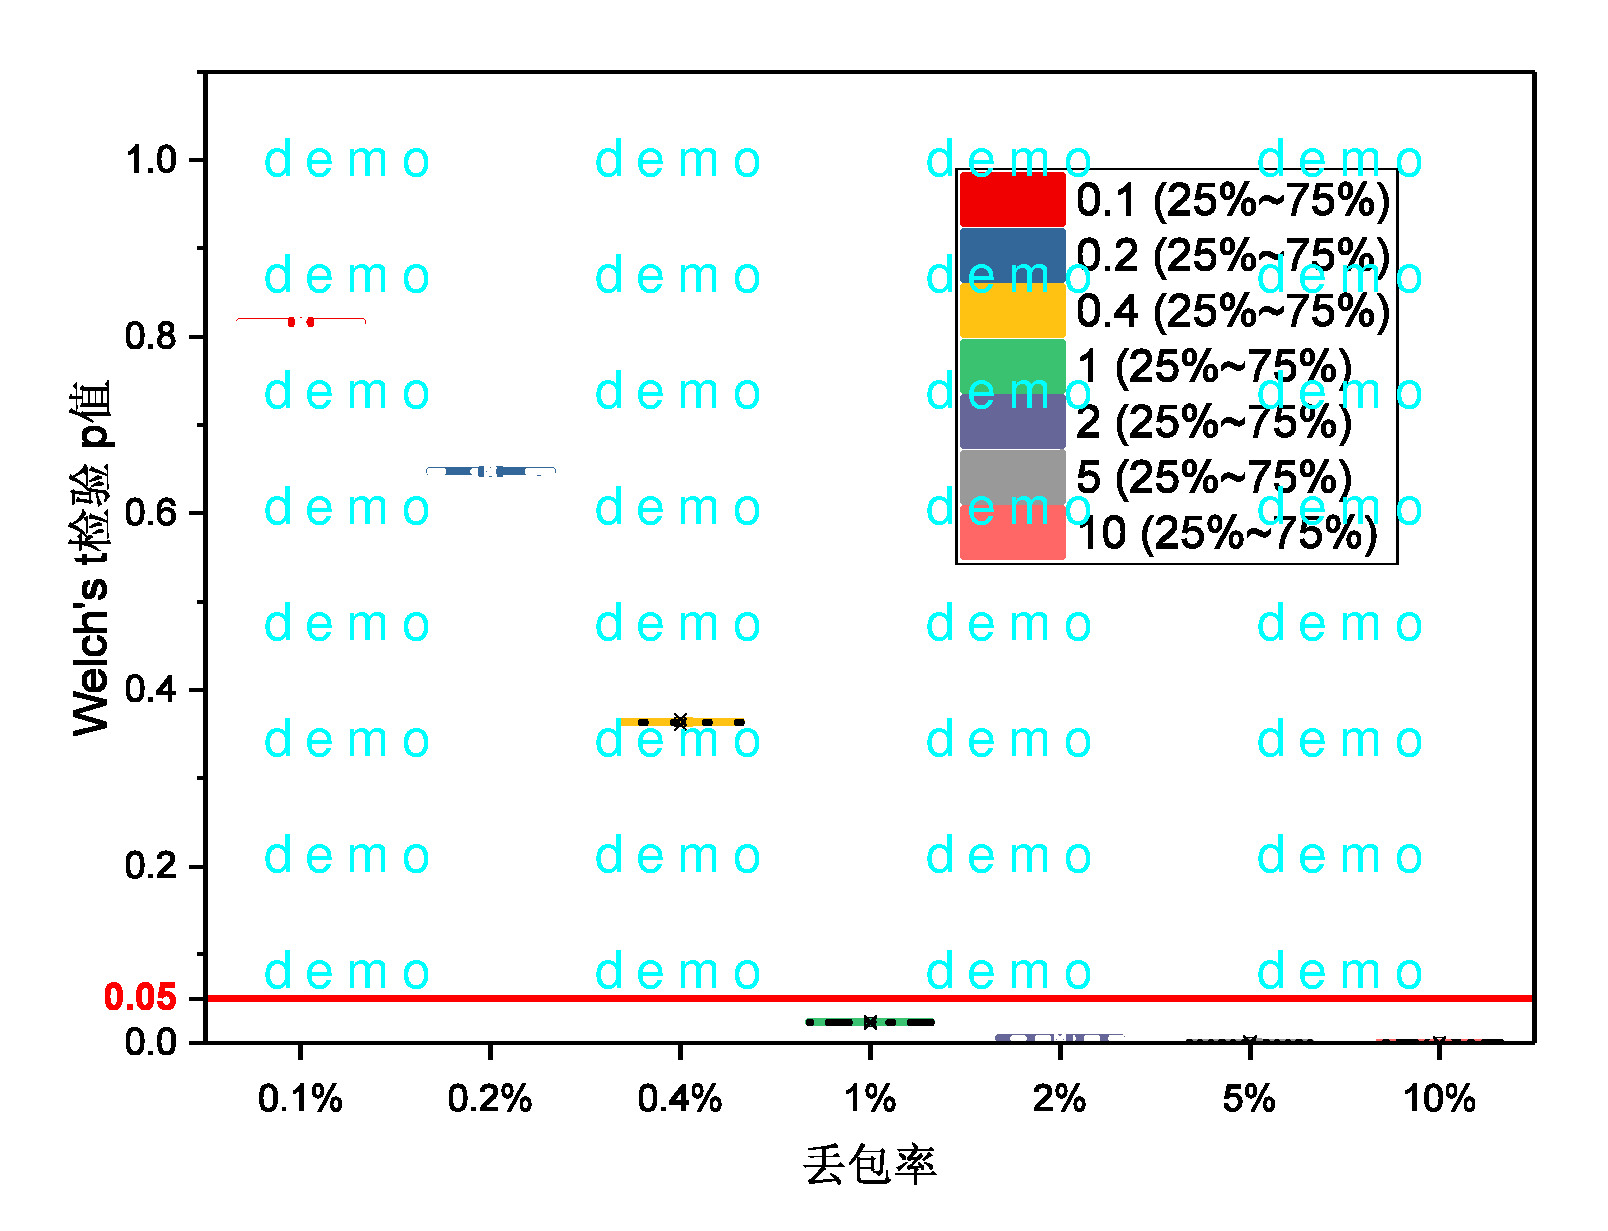
\includegraphics[width=0.48\textwidth]{chapters/chapter3/figures/ipd-t-excellent.pdf}
        }
        \subfigure[Good场景p值的箱线图]{
            \label{fig:3:result:ipd:t:good}
            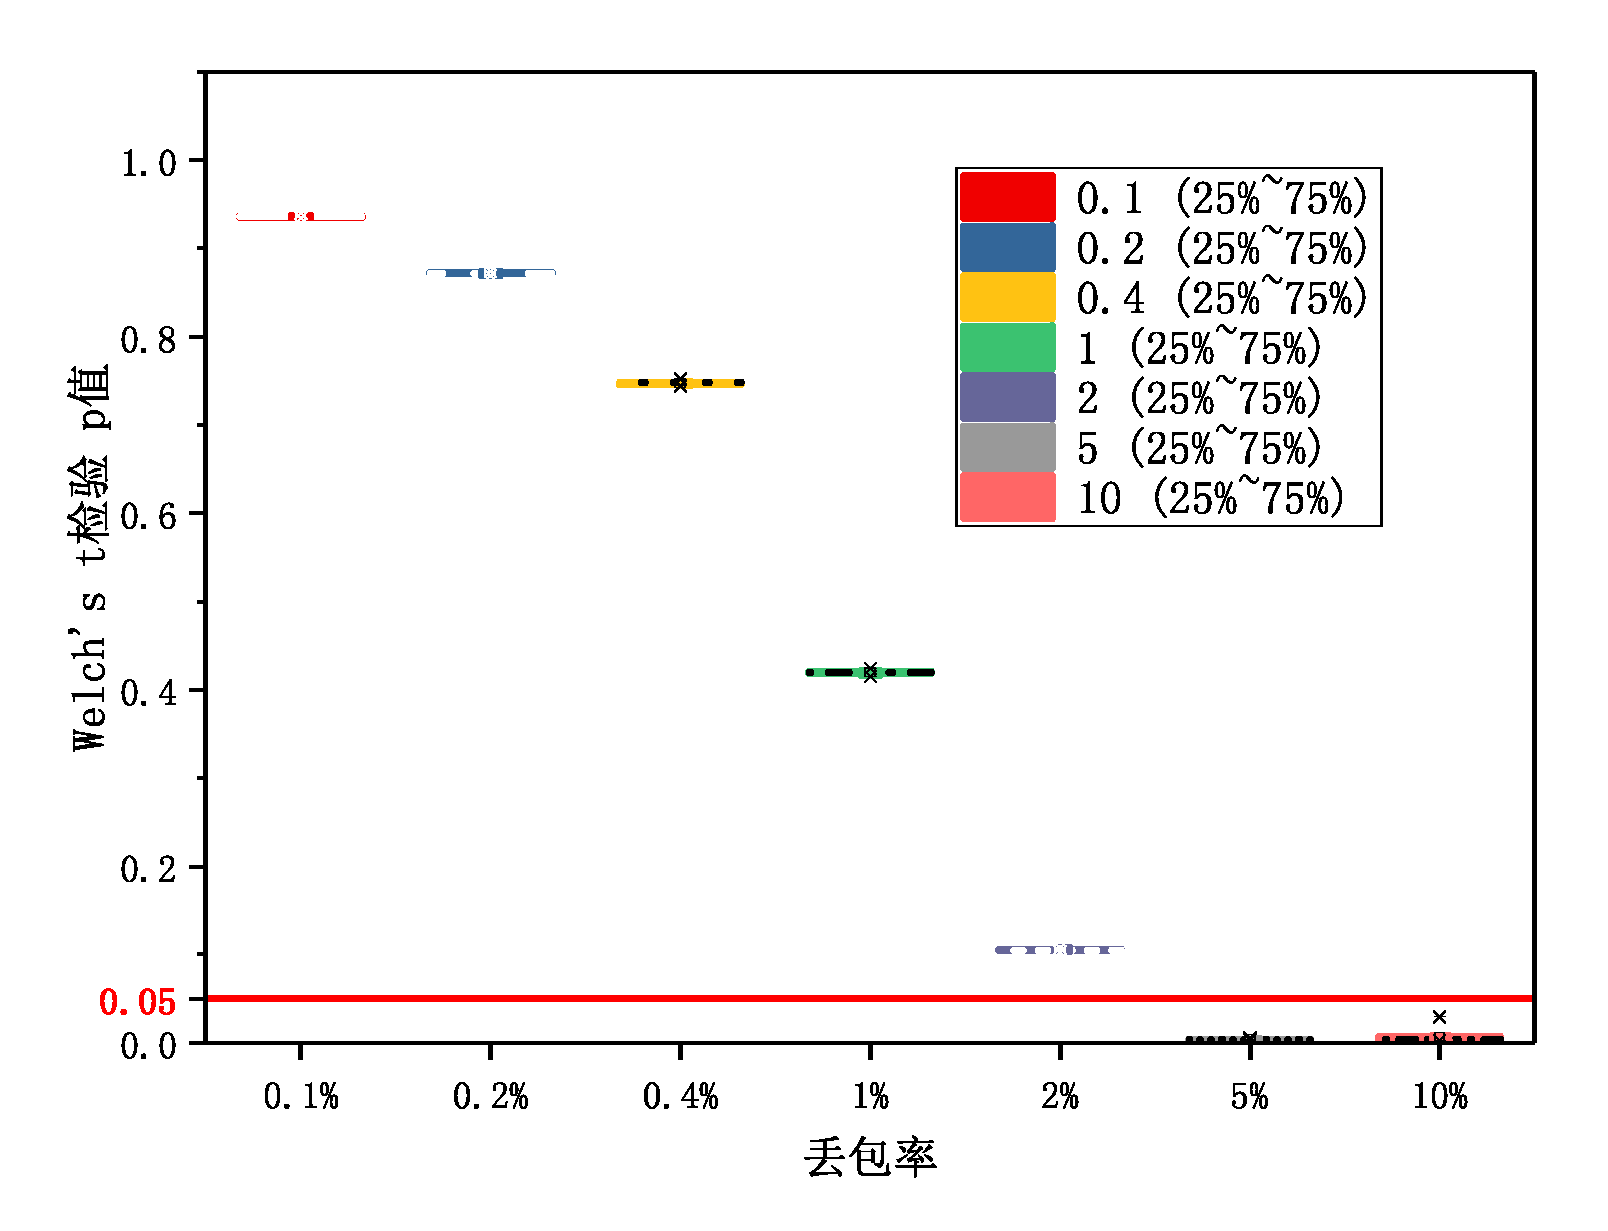
\includegraphics[width=0.48\textwidth]{chapters/chapter3/figures/ipd-t-good.pdf}
        }
        \caption{IPD分布Welch's t检验结果的箱线图}
        \label{fig:3:result:ipd:t}
	\end{figure}
}

\insertFigure{
	\begin{figure}
        \centering
        \subfigure[Excellent场景p值的箱线图]{
            \label{fig:3:result:ipd:mw:excellent}
            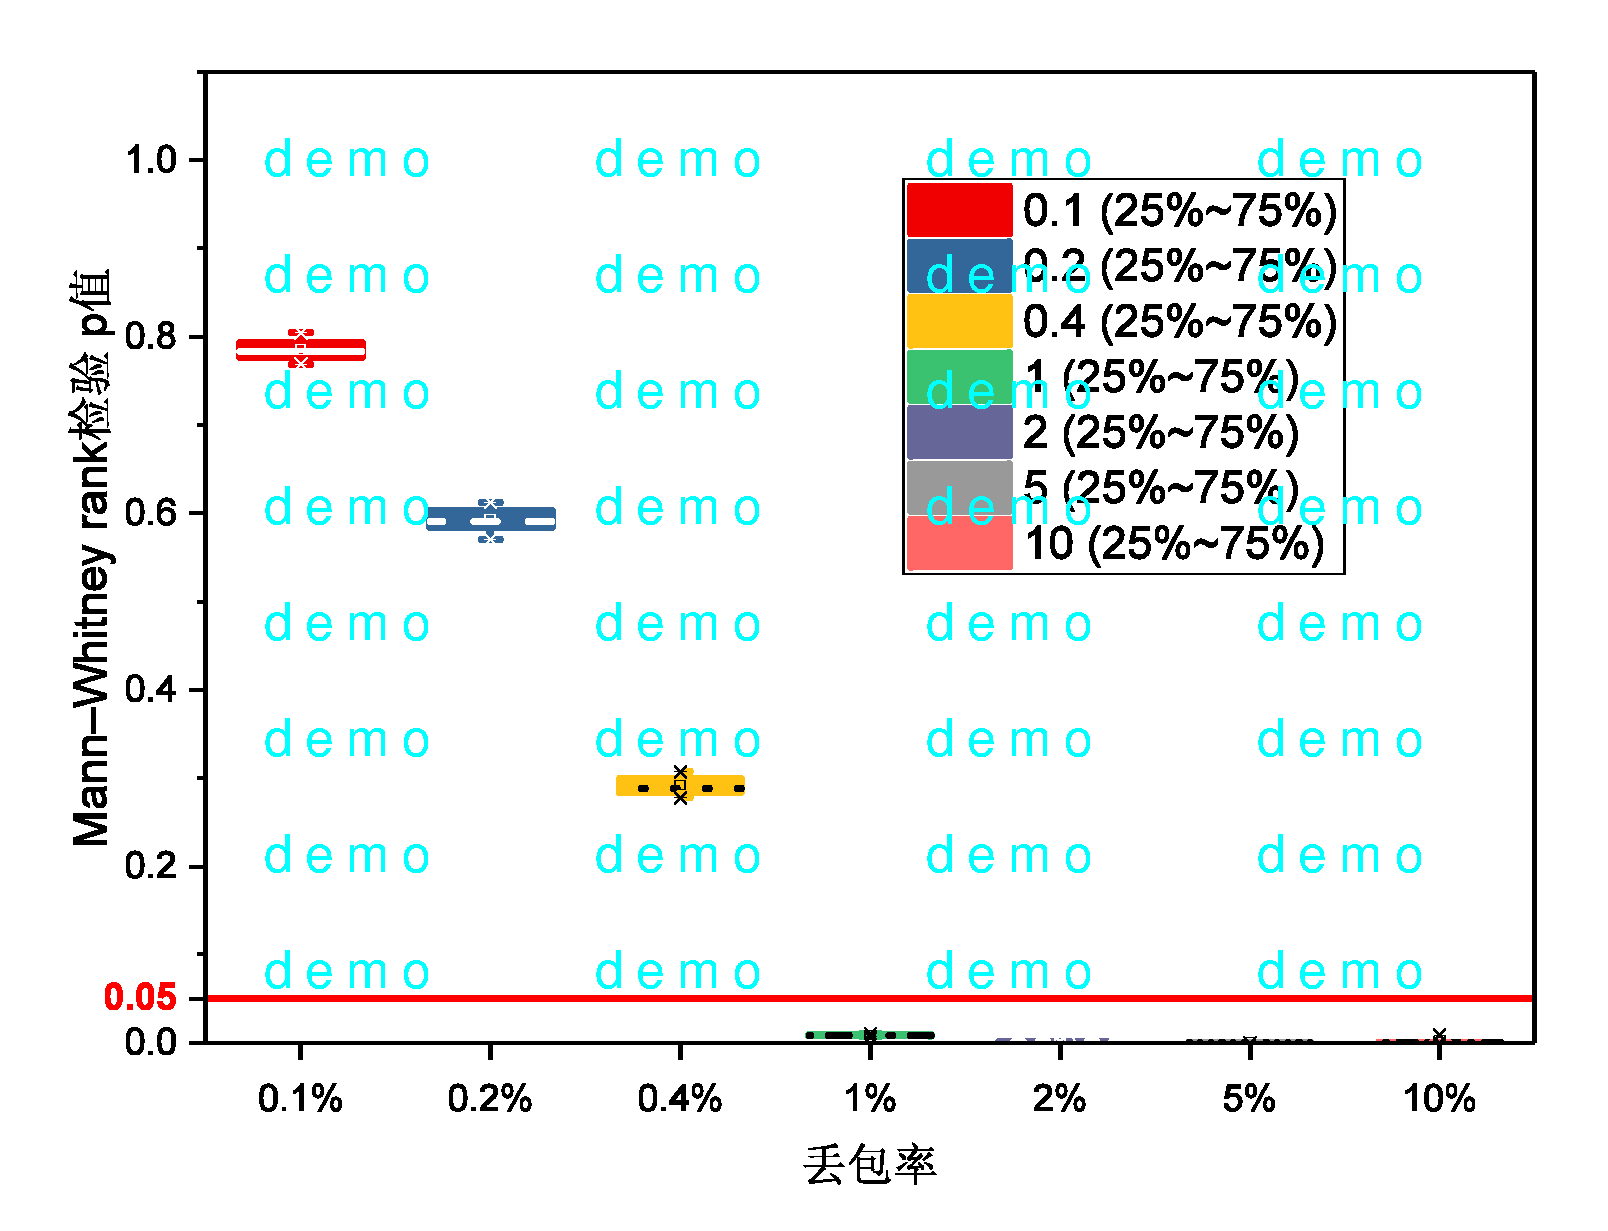
\includegraphics[width=0.48\textwidth]{chapters/chapter3/figures/ipd-mw-excellent.pdf}
        }
        \subfigure[Good场景p值的箱线图]{
            \label{fig:3:result:ipd:mw:good}
            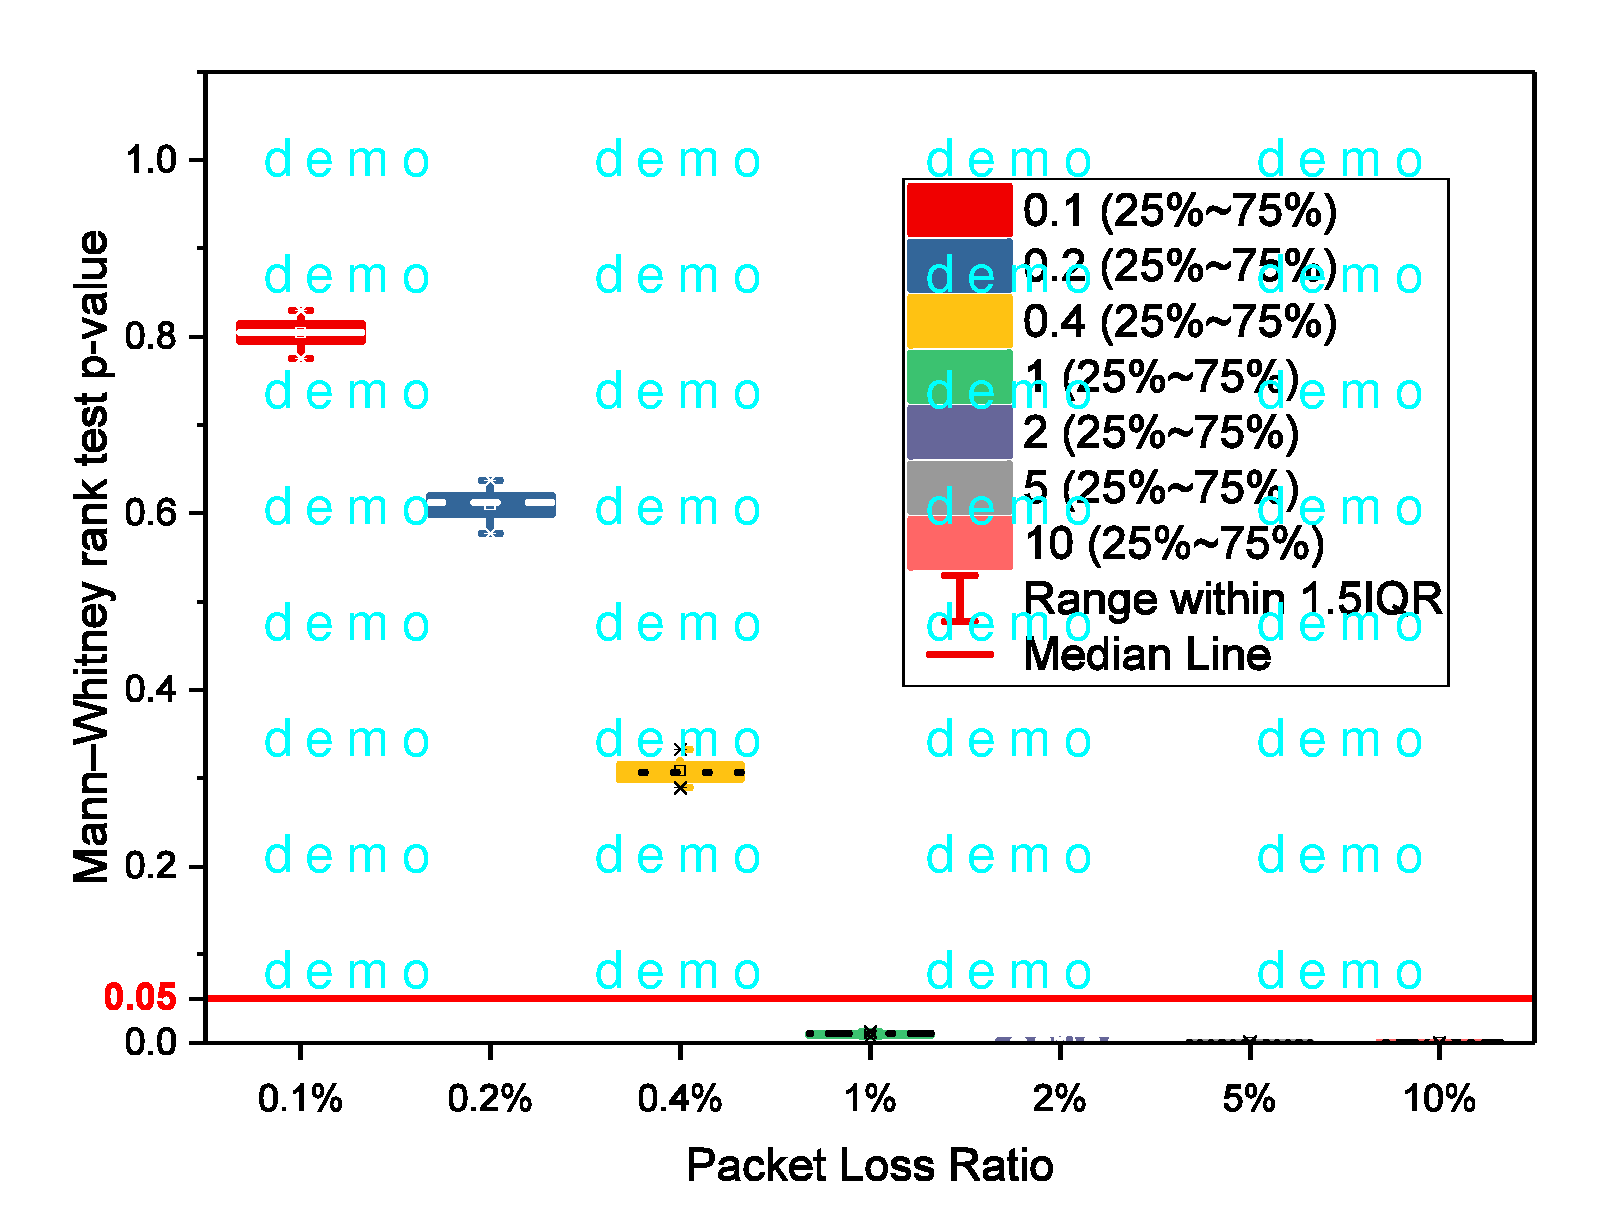
\includegraphics[width=0.48\textwidth]{chapters/chapter3/figures/ipd-mw-good.pdf}
        }
        \caption{IPD分布Mann–Whitney rank检验结果的箱线图}
        \label{fig:3:result:ipd:mw}
	\end{figure}
}

\subsubsection{CDF测试结果}
\label{chap:analyze:result:ipd:cdf}

如图\nref{fig:3:result:ipd:cdf},在CDF趋势方面,时间隐通道的分布虽然出现偏离,但总体趋势仍保持一致。即使随机丢包率上升到10\%,与原始分布的差异也并不明显。因此,时间隐通道的IPD分布可以通过CDF检验,需要其他检测方法进一步检测。

\subsubsection{条件熵测试结果}
\label{chap:analyze:result:ipd:kld}

如图\nref{fig:3:result:ipd:kld},不同测试样本的测试结果被绘制为箱线图。在两种不同的场景中,时间隐通道IPD分布于宿主信道IPD分布,进行K-L散度测试后,结果均小于阈值0.1。并且,随着主动丢包率的降低,K-L散度逐渐下降,意味着隐通道的IPD分布于宿主信道的IPD分布更加接近。

从检测效果来看,在IPD分布中,时间隐通道与宿主信道十分接近,CDF检测及K-L散度均无法识别,需要进一步采用一致性检验进行判断。

\subsubsection{一致性检验测试结果}
\label{chap:analyze:result:ipd:statistical}

如图\nref{fig:3:result:ipd:ks},在K-S检验中,已经能够检测出IPD分布的不一致现象。当丢包率$\le 1\%$时,Excellent场景下已经基本通过了K-S检验,随着PLR的进一步降低,K-S检验的p值逐渐增大。如图\nref{fig:3:result:ipd:t},在Welch's t检验中,两种场景下的检测结果出现差异。在Excellent场景中,当丢包率$\le 0.4\%$后,才可以通过Welch's t检验;而在Good场景中,当丢包率$\le 2\%$时,即可通过Welch's t检验。Welch's t检验结果证明,在不同的场景中,丢包导致的IPD平均值变化程度不同。

如图\nref{fig:3:result:ipd:mw},在Mann–Whitney rank检验中,两种场景下只有丢包率$\le 0.4\%$才可通过测试。由于Mann–Whitney rank检验适用分布为正态分布,而IPD分布与标准的正态分布偏差较大,所以检验结果较Welch's t检验要更加严格。

\insertFigure{
	\begin{figure}
        \centering
        \subfigure[Excellent场景相对距离的箱线图]{
            \label{fig:3:result:ipd:wd:excellent}
            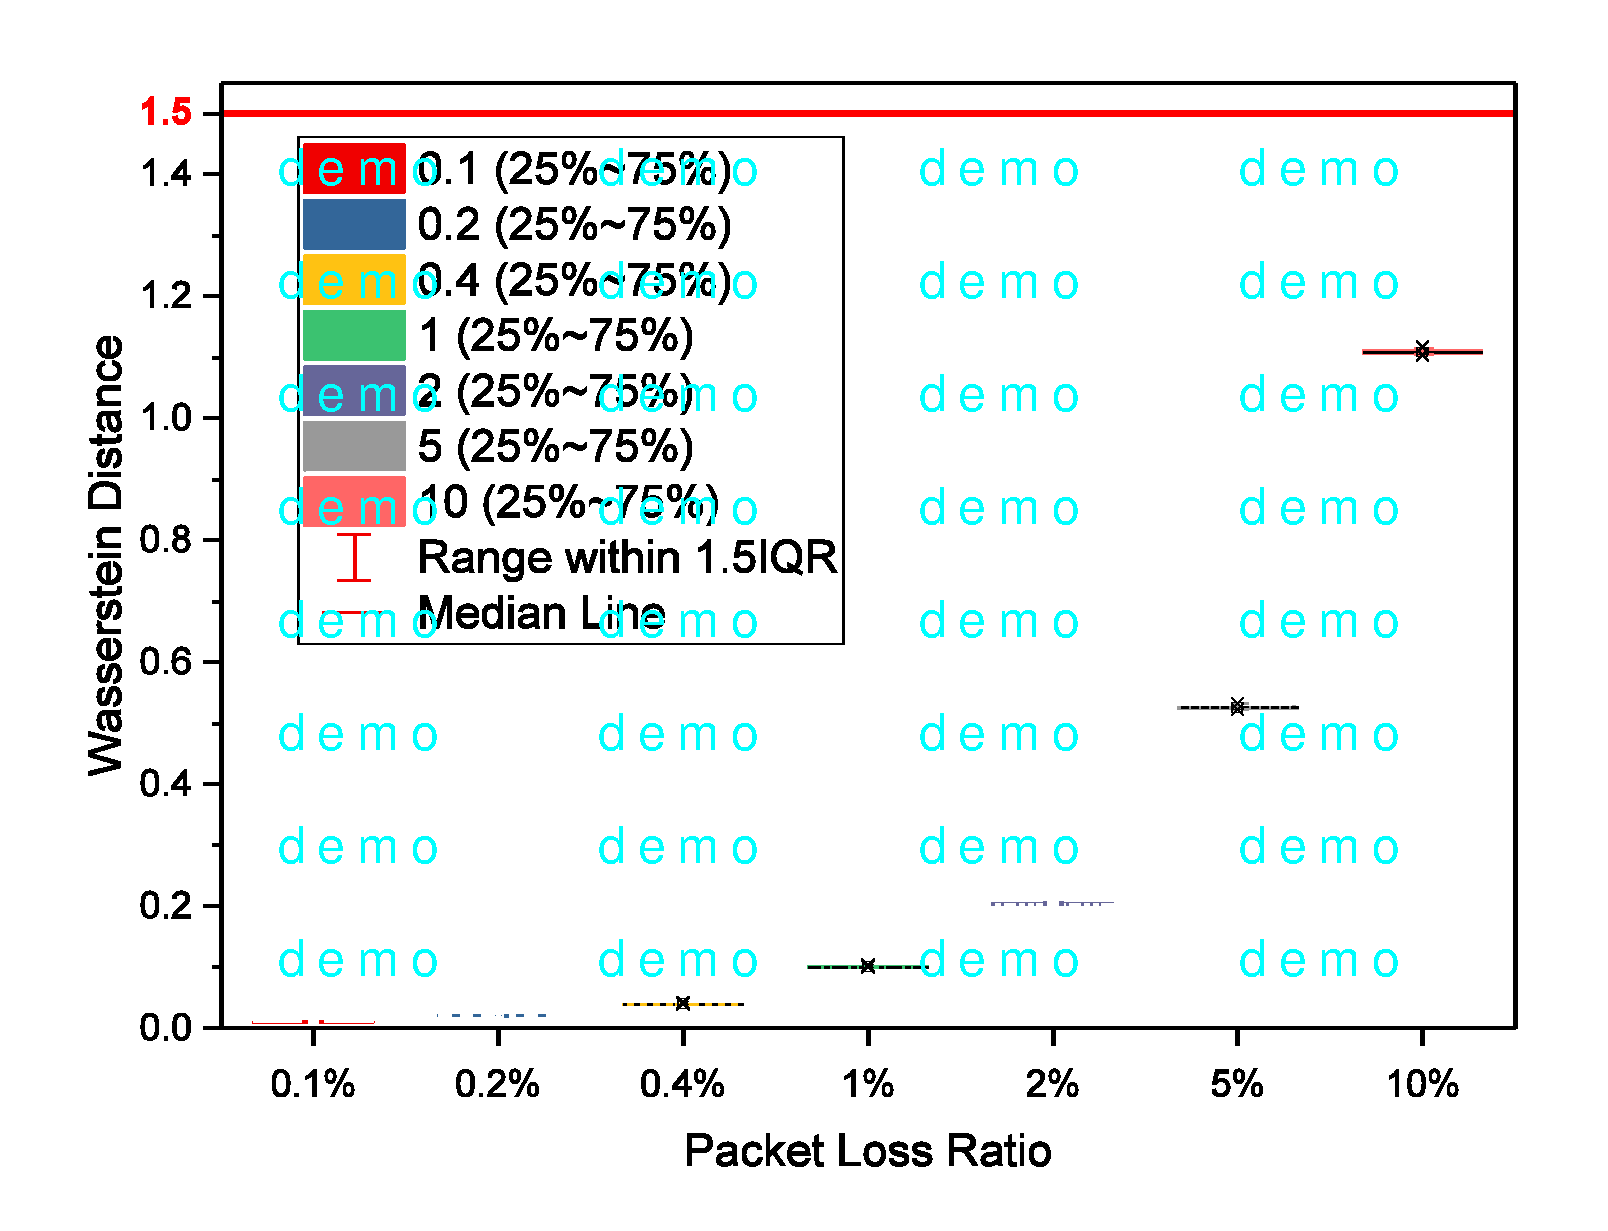
\includegraphics[width=0.48\textwidth]{chapters/chapter3/figures/ipd-wd-excellent.pdf}
        }
        \subfigure[Good场景相对距离的箱线图]{
            \label{fig:3:result:ipd:wd:good}
            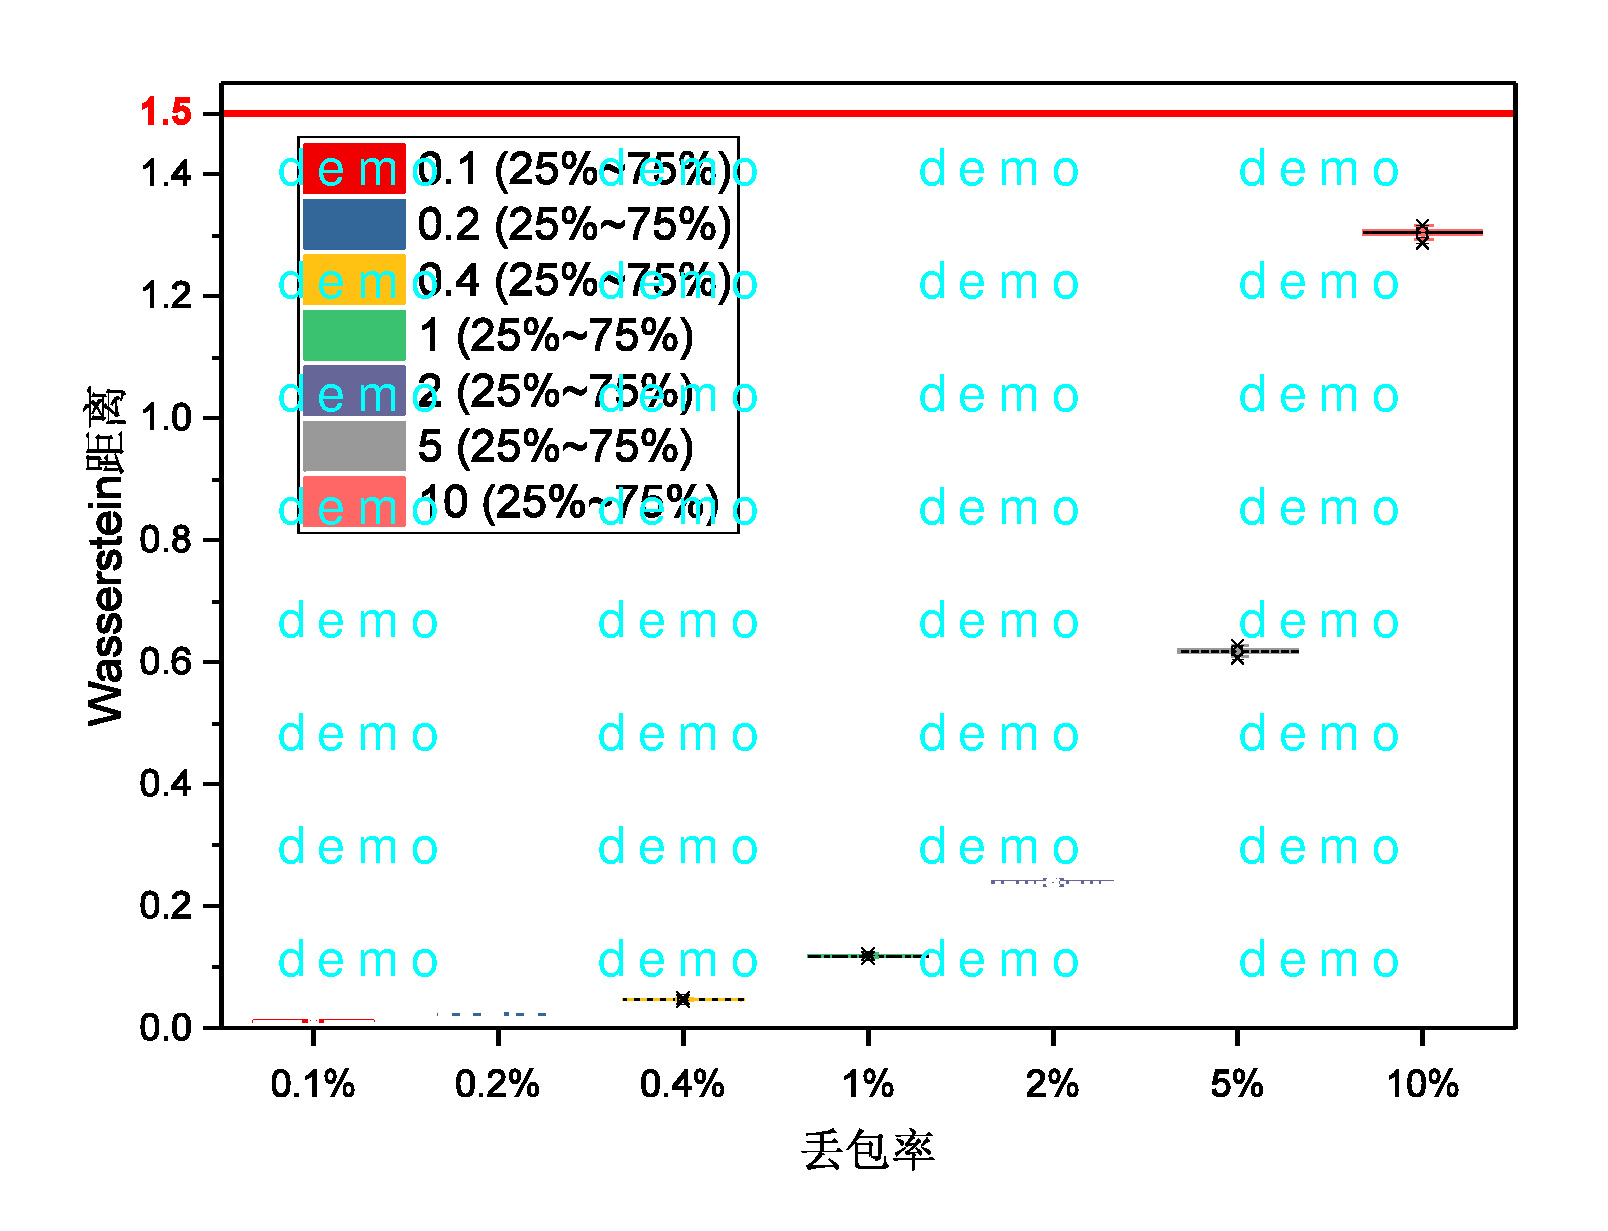
\includegraphics[width=0.48\textwidth]{chapters/chapter3/figures/ipd-wd-good.pdf}
        }
        \caption{IPD分布Wasserstein距离的箱线图}
        \label{fig:3:result:ipd:wd}
	\end{figure}
}

\subsubsection{相对距离测试结果}
\label{chap:analyze:result:ipd:distance}

\insertFigure{
	\begin{figure}
        \centering
        \subfigure[Excellent场景相对距离的箱线图]{
            \label{fig:3:result:ipd:ed:excellent}
            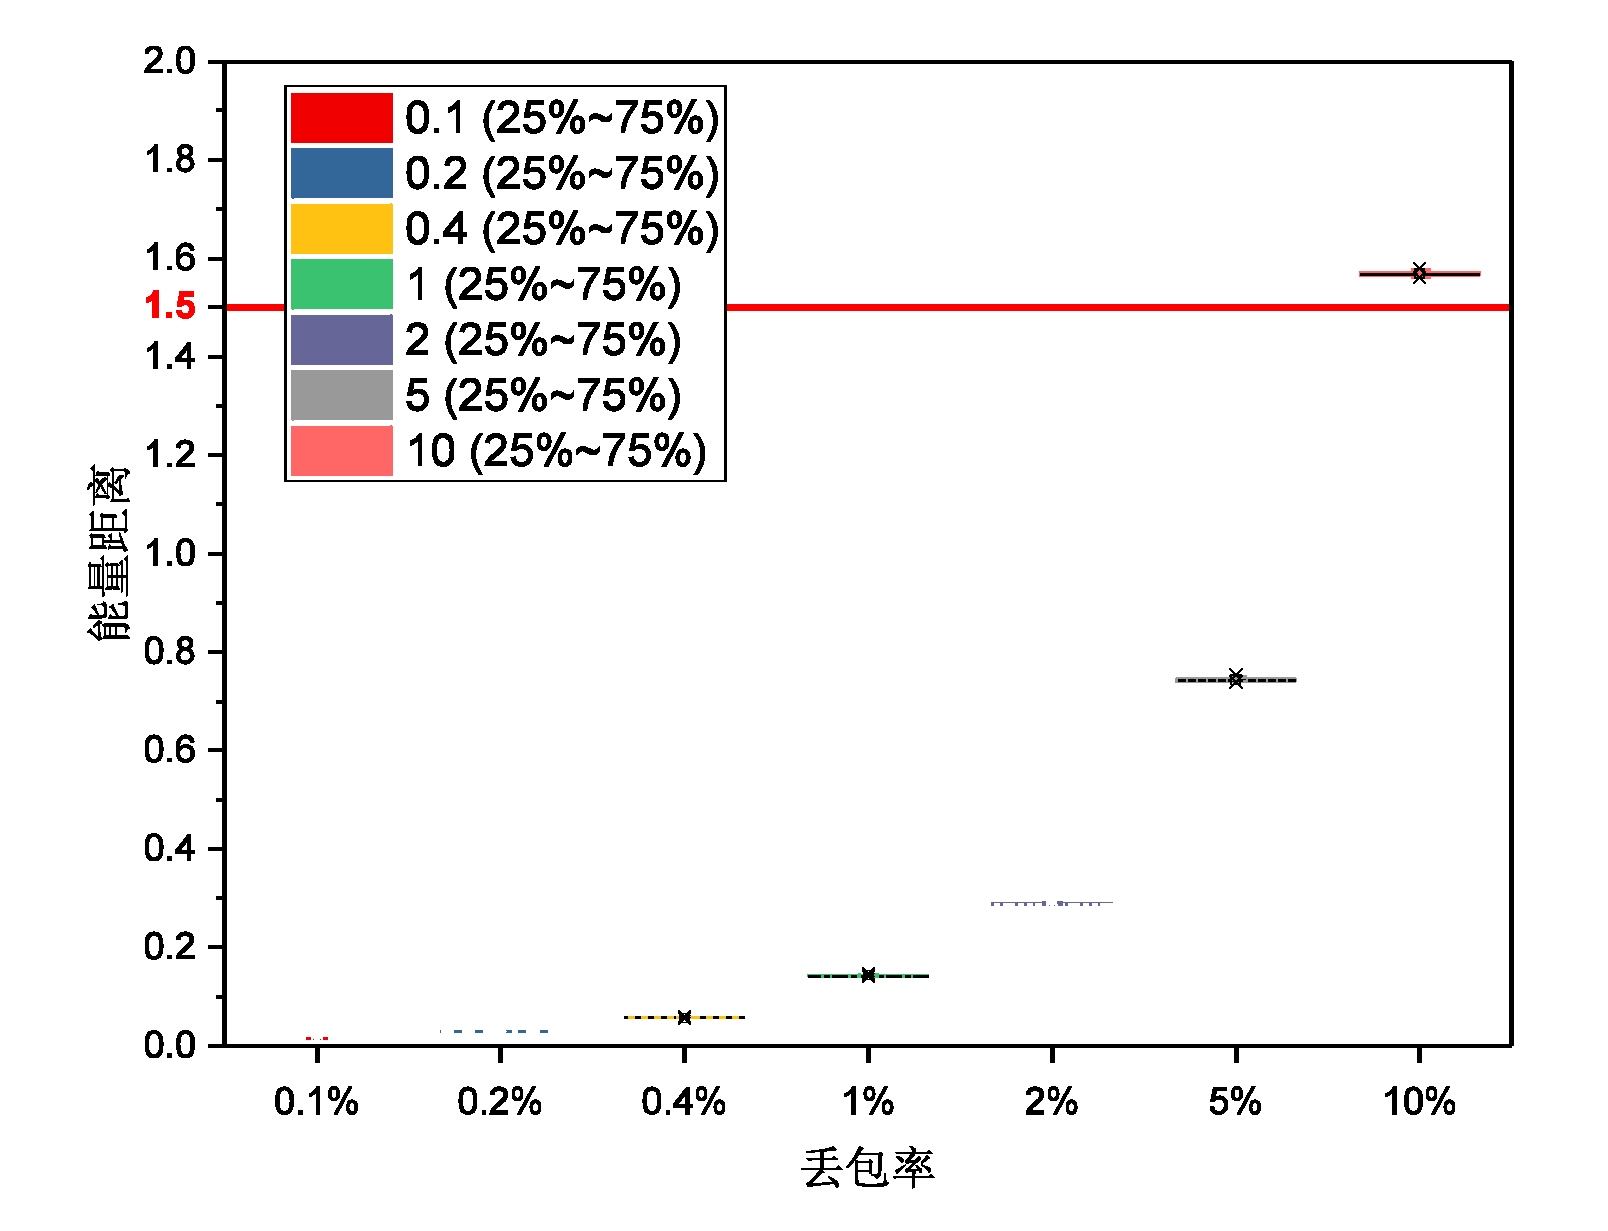
\includegraphics[width=0.48\textwidth]{chapters/chapter3/figures/ipd-ed-excellent.pdf}
        }
        \subfigure[Good场景相对距离的箱线图]{
            \label{fig:3:result:ipd:ed:good}
            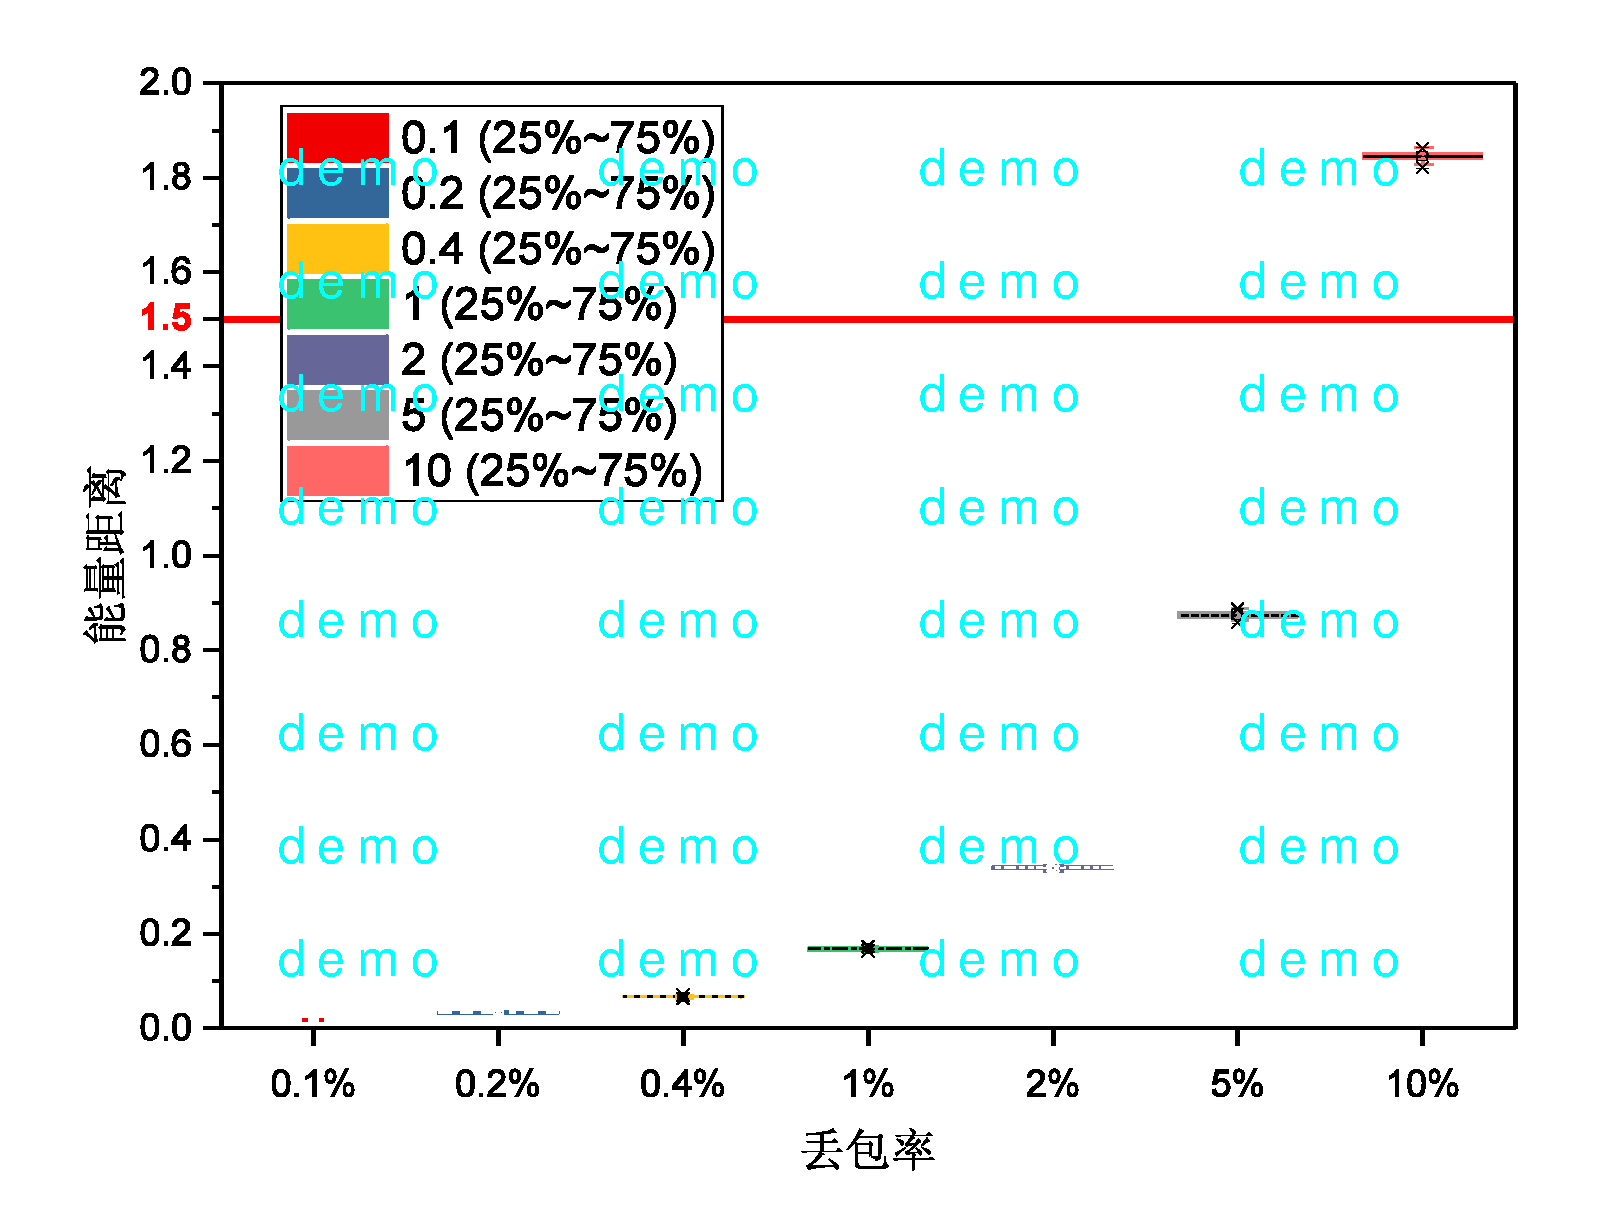
\includegraphics[width=0.48\textwidth]{chapters/chapter3/figures/ipd-ed-good.pdf}
        }
        \caption{IPD分布能量距离的箱线图}
        \label{fig:3:result:ipd:ed}
	\end{figure}
}

如图\nref{fig:3:result:ipd:wd},PLR与Wasserstein距离存在一定的关联关系,随着PLR的增大,相对距离也随之增大。在两种场景中,检测结果是相同的,虽然在丢包率$=10\%$已经接近判断阈值,但仍未超过,因此无法检测出时间隐通道。如图\nref{fig:3:result:ipd:ed},能量距离的计算结果与PLR也呈现正相关,在两种场景中,当丢包率$\le 5\%$时,才可以通过能量距离检测。由结果来看,能量距离较Wasserstein距离具有更高的要求,但二者的总体趋势是基本一致的。

通过以上测试可以发现,通过IPD检测基于主动丢包的时间隐通道,在灵敏度方面无法达到隐通道的检测要求。主要的因素,在于丢包事件与IPD相比数量较少,少量的丢包很难影响IPD分布出现大的变动,因此现有基于IPD的时间隐通道检测方法,无法满足本论文的检测要求,需要结合丢包特征方面的检测方法。

\subsection{突发丢包长度测试结果评估}
\label{chap:analyze:result:burst}

本节介绍的是对突发丢包长度的测试结果,在基于主动丢包的时间隐通道中,对丢包分布产生的影响是最明显的。因此,该检验方法能够弥补IPD分布检测的不足。

\insertFigure{
	\begin{figure}
        \centering
        \subfigure[Excellent场景的CDF]{
            \label{fig:3:result:burst:cdf:excellent}
            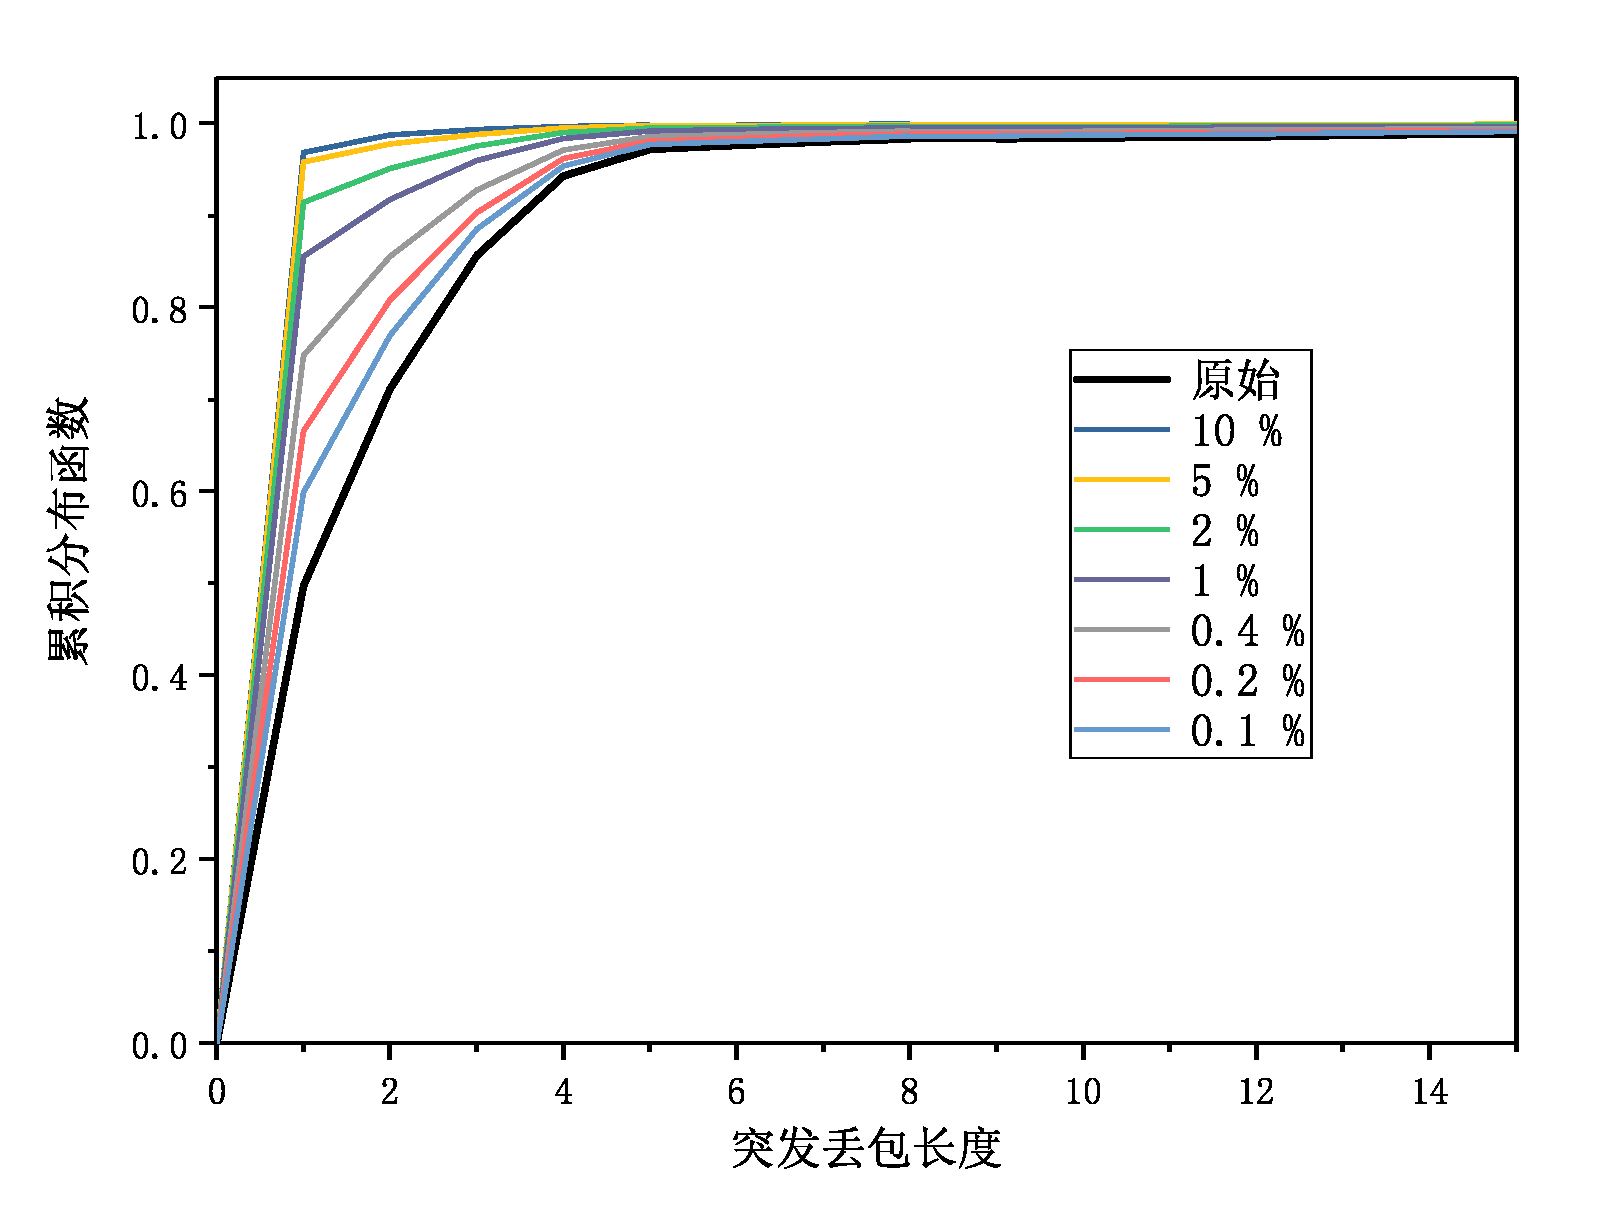
\includegraphics[width=0.48\textwidth]{chapters/chapter3/figures/burst-cdf-excellent.pdf}
        }
        \subfigure[Good场景的CDF]{
            \label{fig:3:result:burst:cdf:good}
            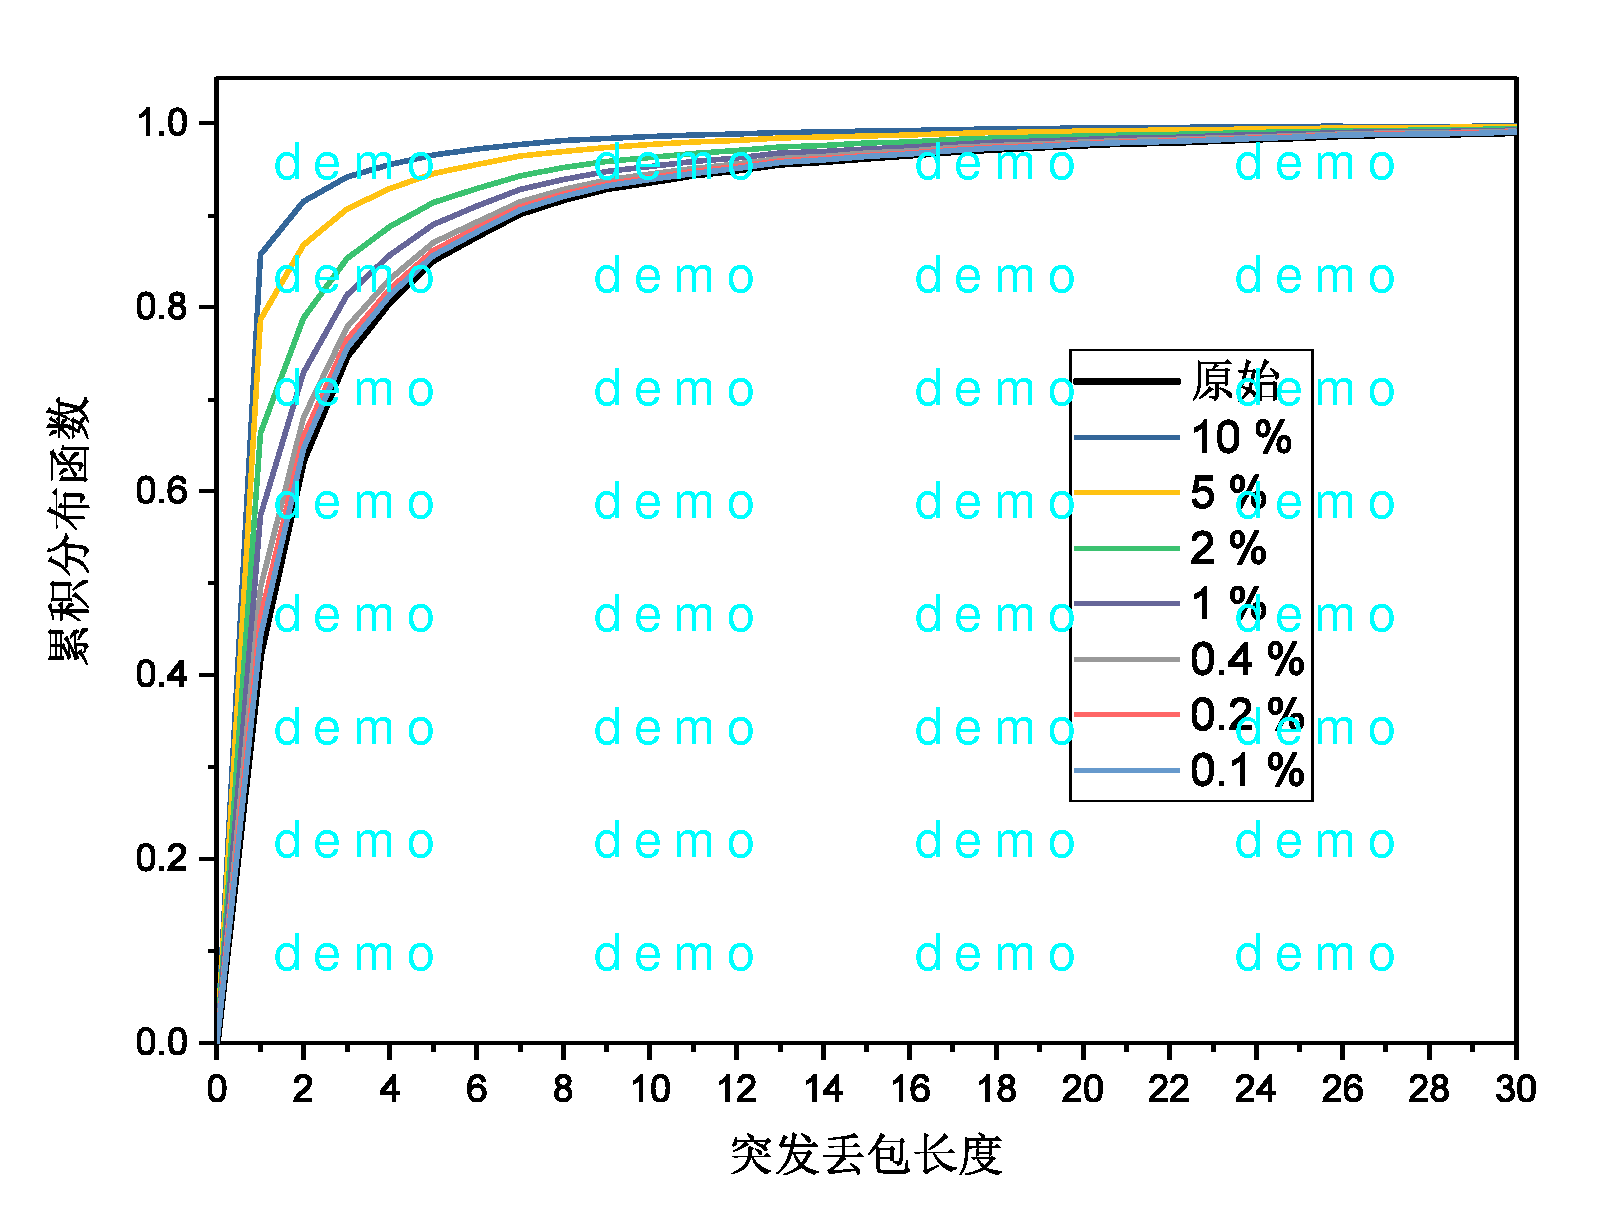
\includegraphics[width=0.48\textwidth]{chapters/chapter3/figures/burst-cdf-good.pdf}
        }
        \caption{突发丢包长度的CDF曲线}
        \label{fig:3:result:burst:cdf}
	\end{figure}
}

\insertFigure{
	\begin{figure}
        \centering
        \subfigure[Excellent场景K-L散度的箱线图]{
            \label{fig:3:result:burst:kld:excellent}
            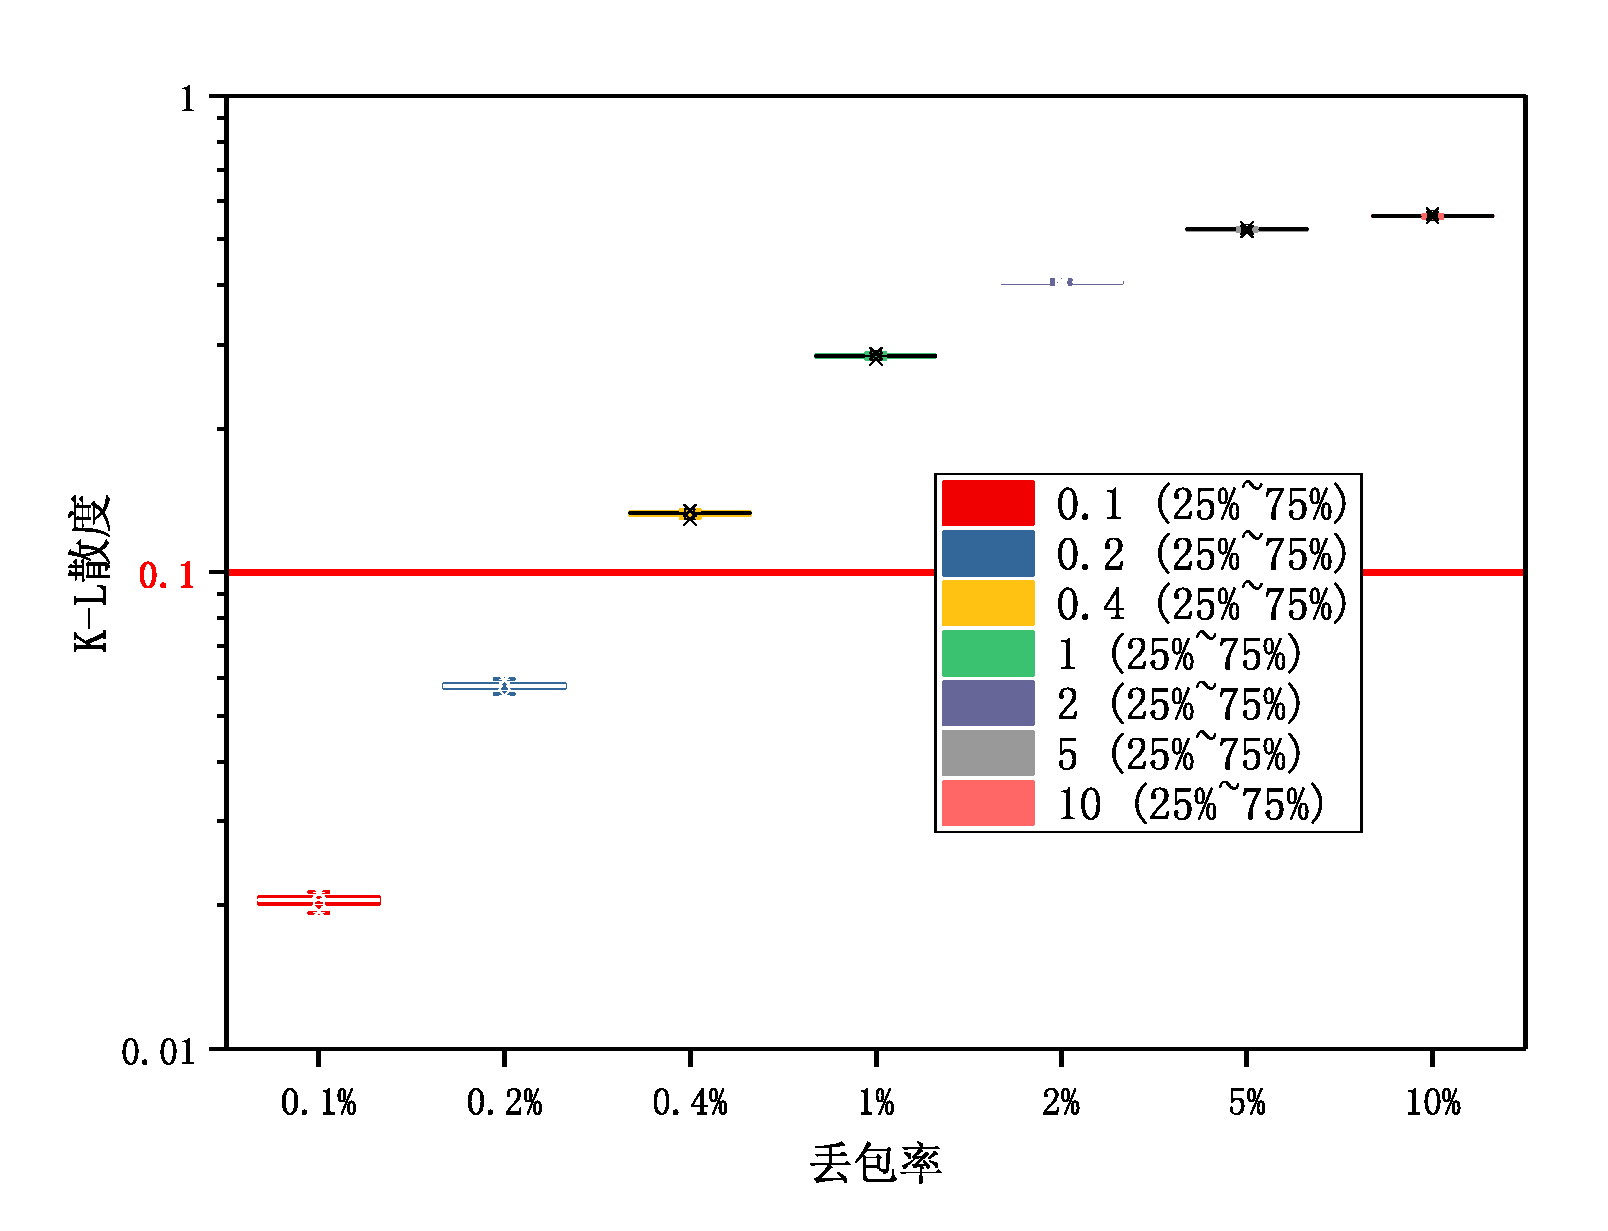
\includegraphics[width=0.48\textwidth]{chapters/chapter3/figures/burst-kld-excellent.pdf}
        }
        \subfigure[Good场景K-L散度的箱线图]{
            \label{fig:3:result:burst:kld:good}
            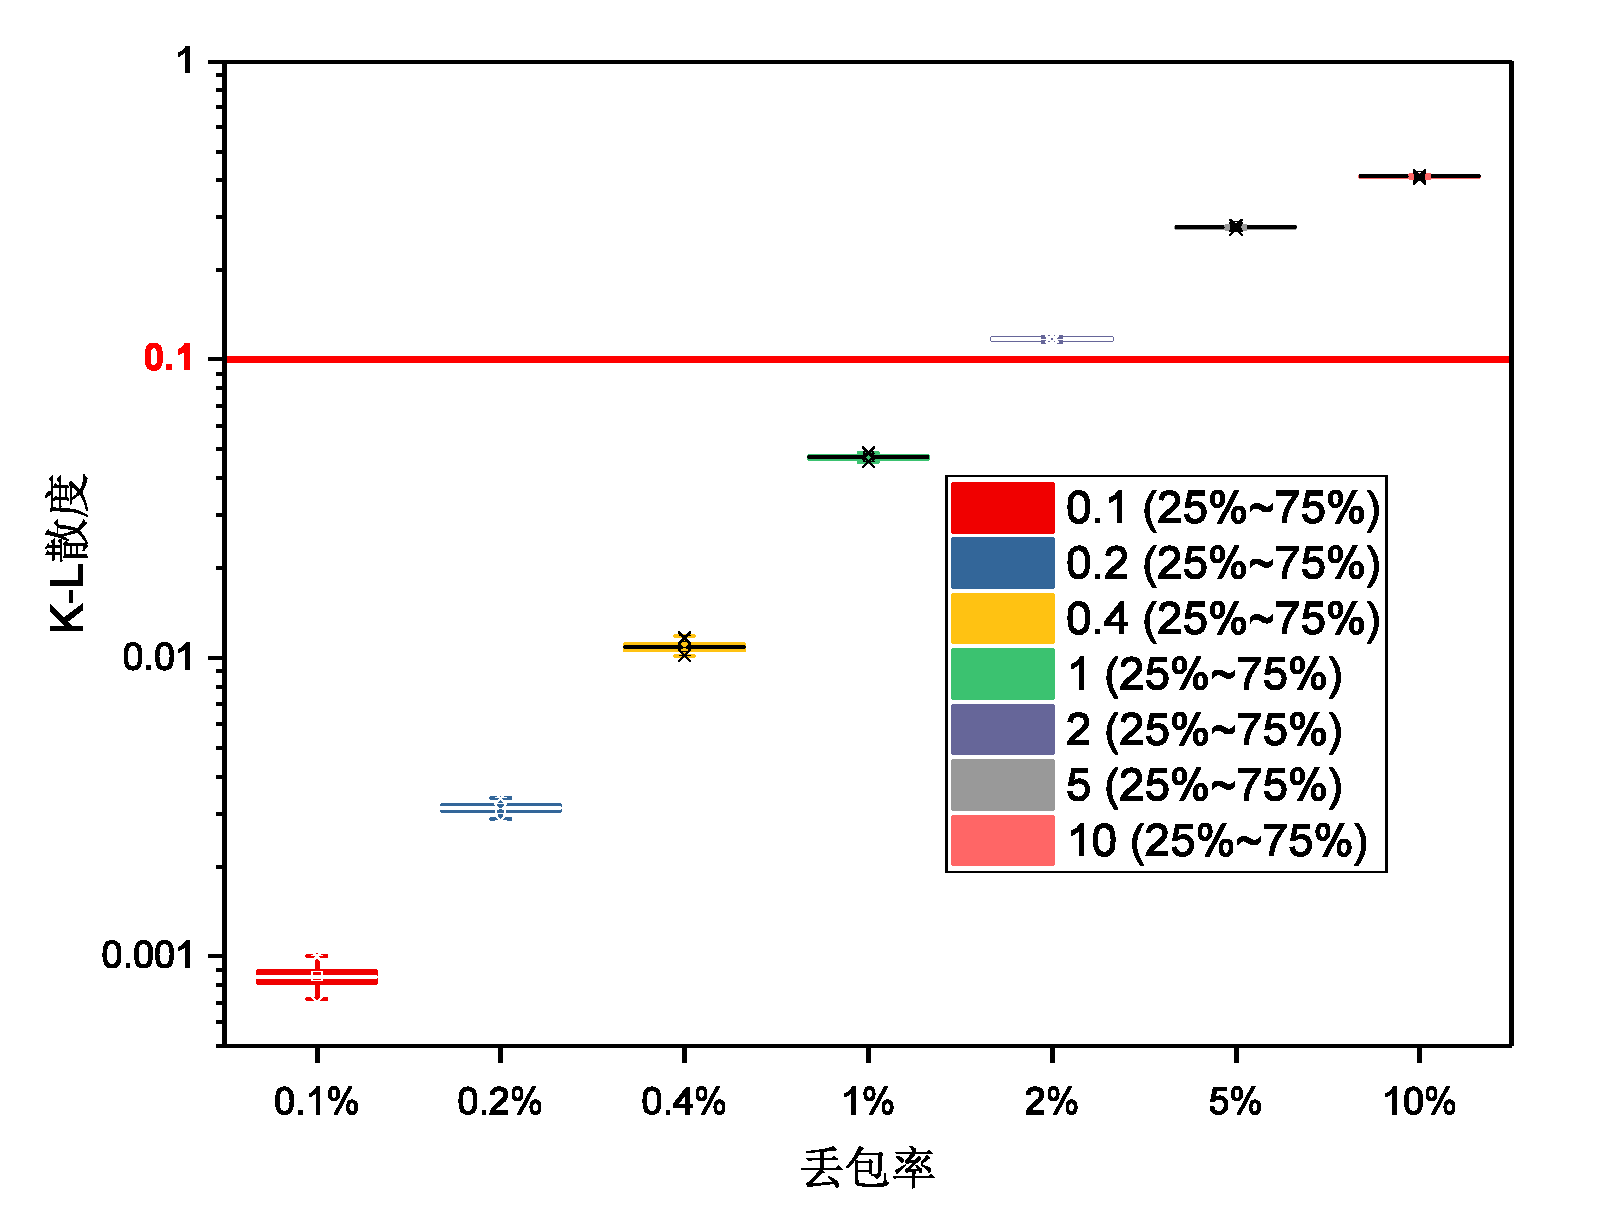
\includegraphics[width=0.48\textwidth]{chapters/chapter3/figures/burst-kld-good.pdf}
        }
        \caption{突发丢包长度K-L散度测试的箱线图}
        \label{fig:3:result:burst:kld}
	\end{figure}
}

\insertFigure{
	\begin{figure}
        \centering
        \subfigure[Excellent场景Wasserstein距离的箱线图]{
            \label{fig:3:result:burst:wd:excellent}
            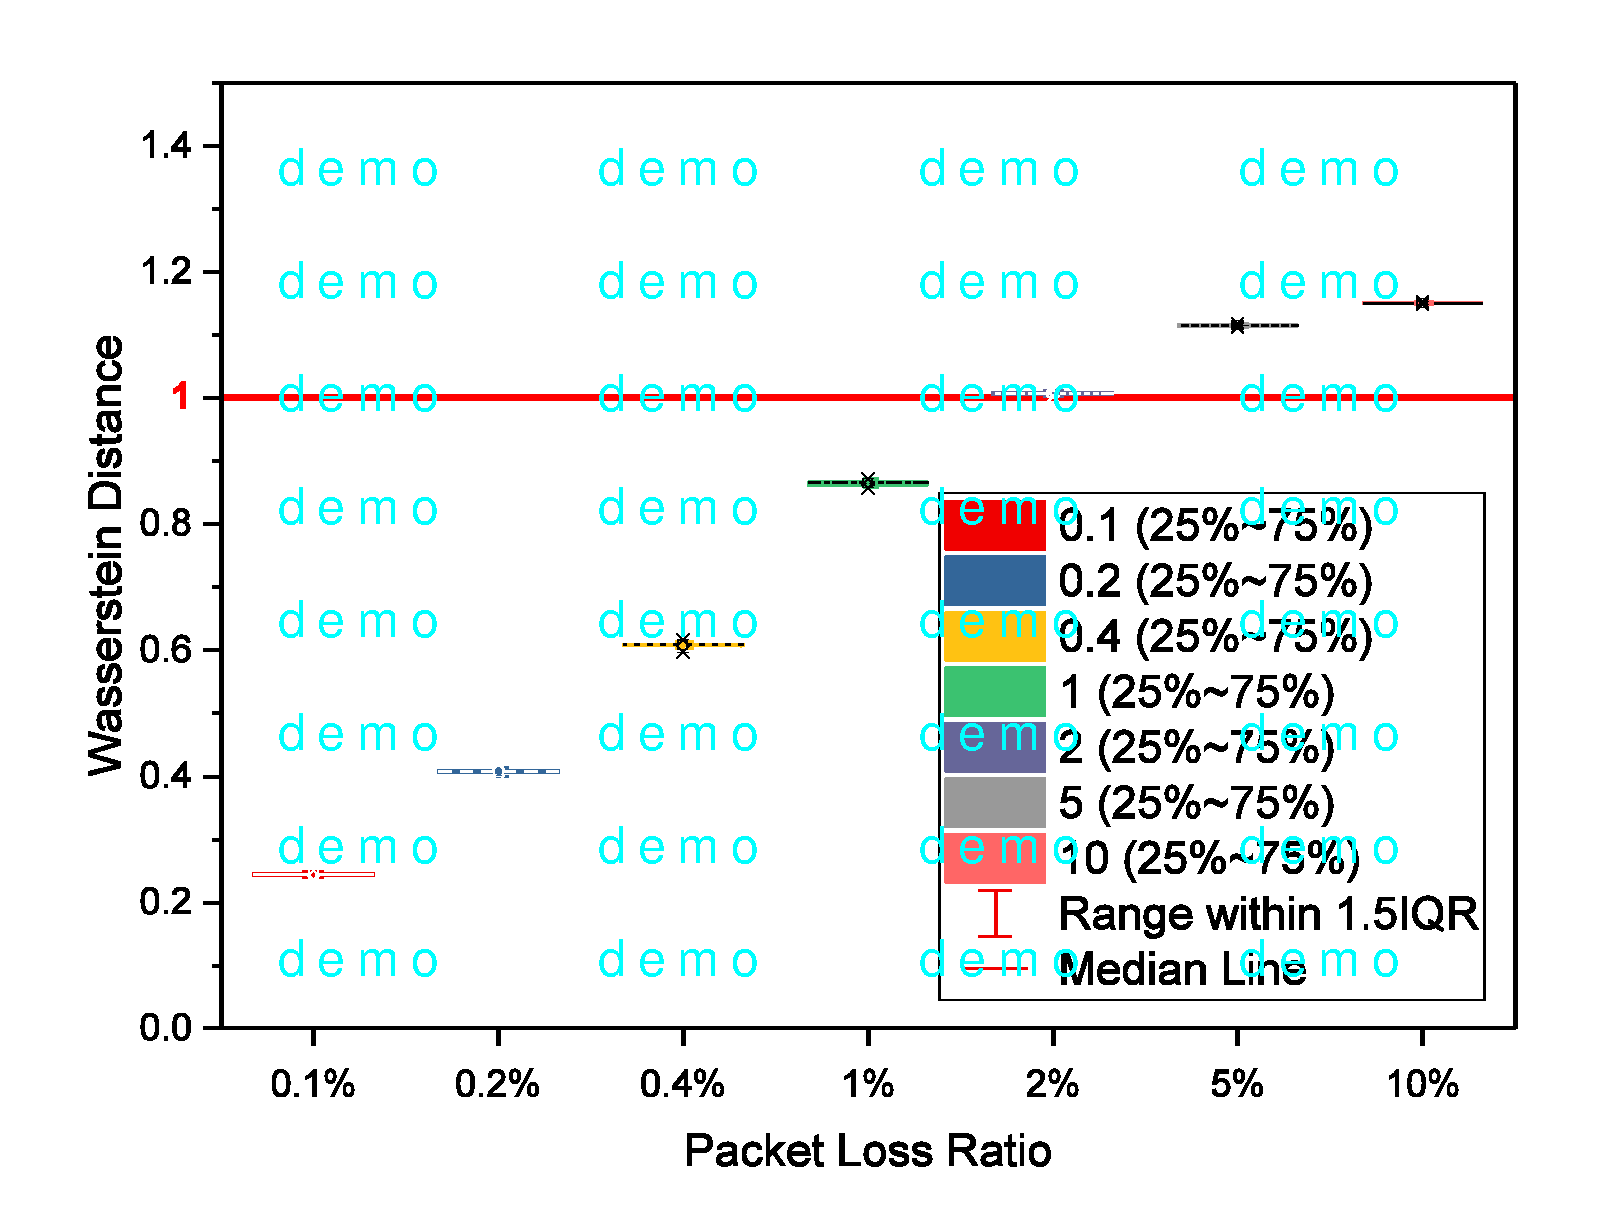
\includegraphics[width=0.48\textwidth]{chapters/chapter3/figures/burst-wd-excellent.pdf}
        }
        \subfigure[Good场景Wasserstein距离的箱线图]{
            \label{fig:3:result:burst:wd:good}
            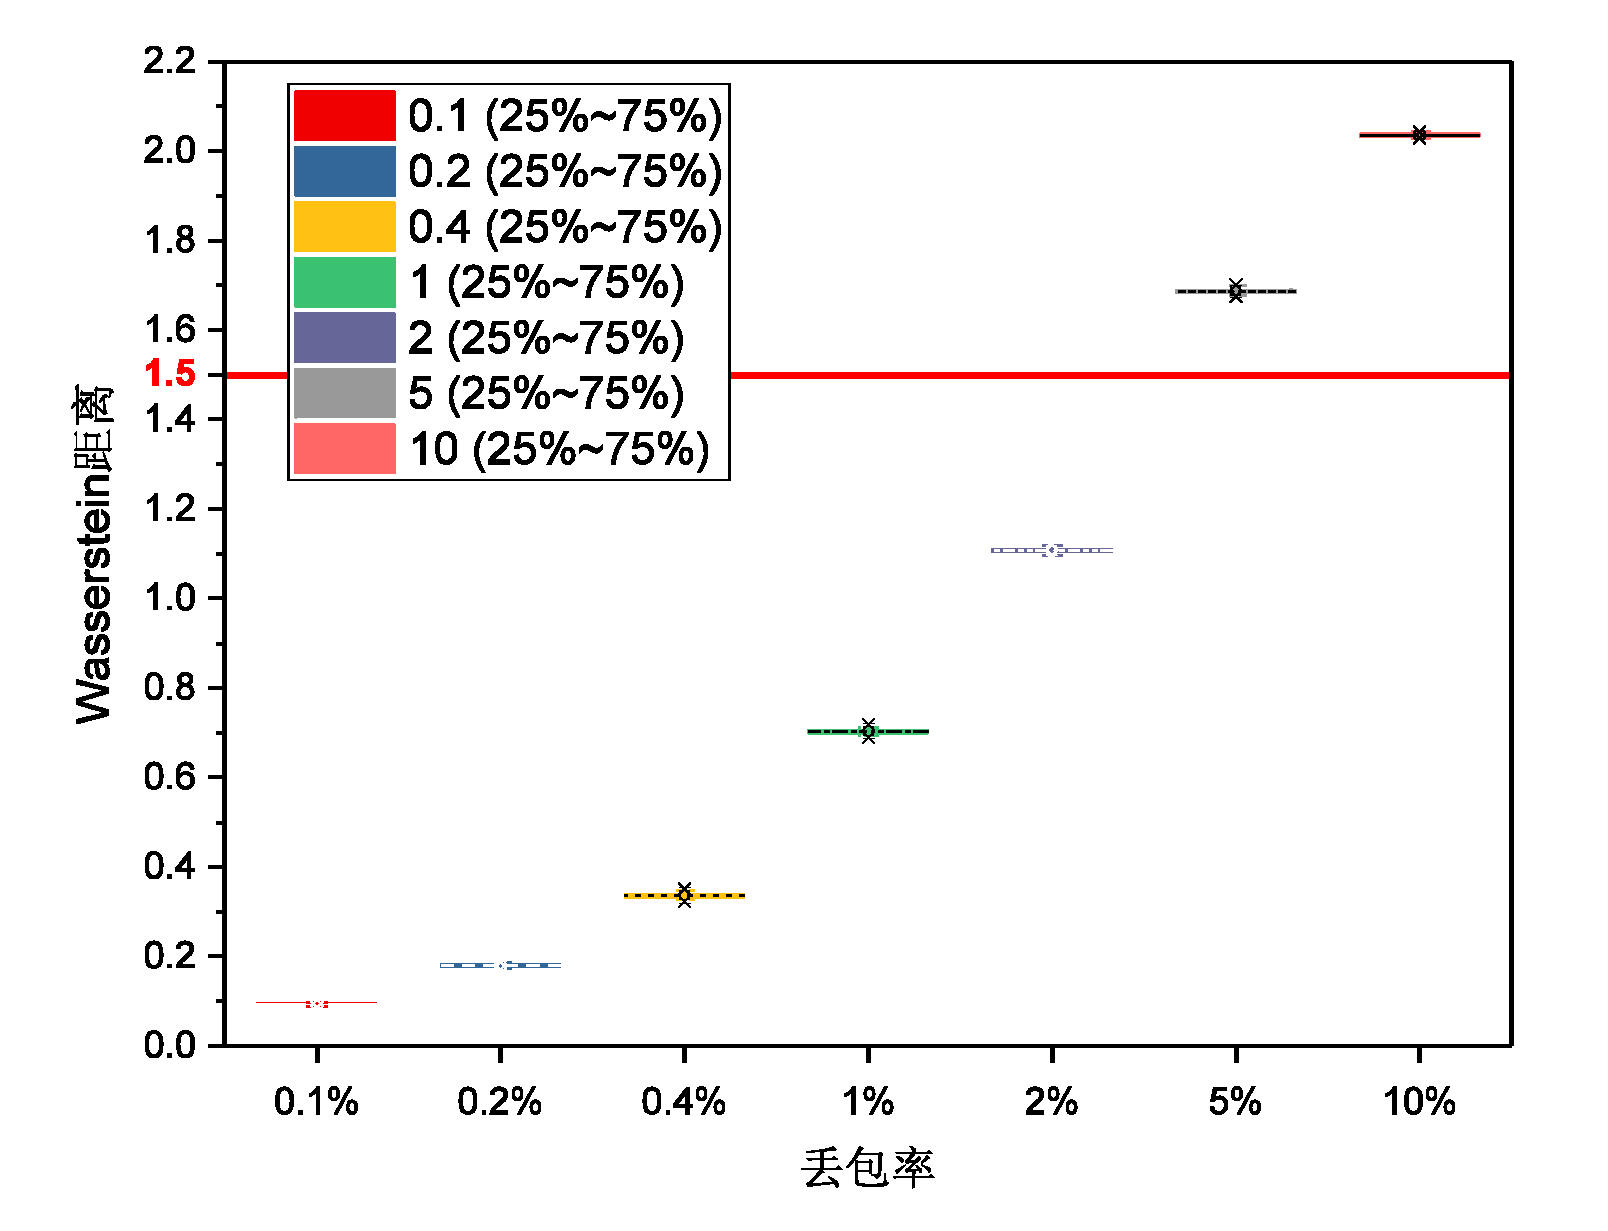
\includegraphics[width=0.48\textwidth]{chapters/chapter3/figures/burst-wd-good.pdf}
        }
        \caption{突发丢包长度Wasserstein距离的箱线图}
        \label{fig:3:result:burst:wd}
	\end{figure}
}

\insertFigure{
	\begin{figure}
        \centering
        \subfigure[Excellent场景能量距离的箱线图]{
            \label{fig:3:result:burst:ed:excellent}
            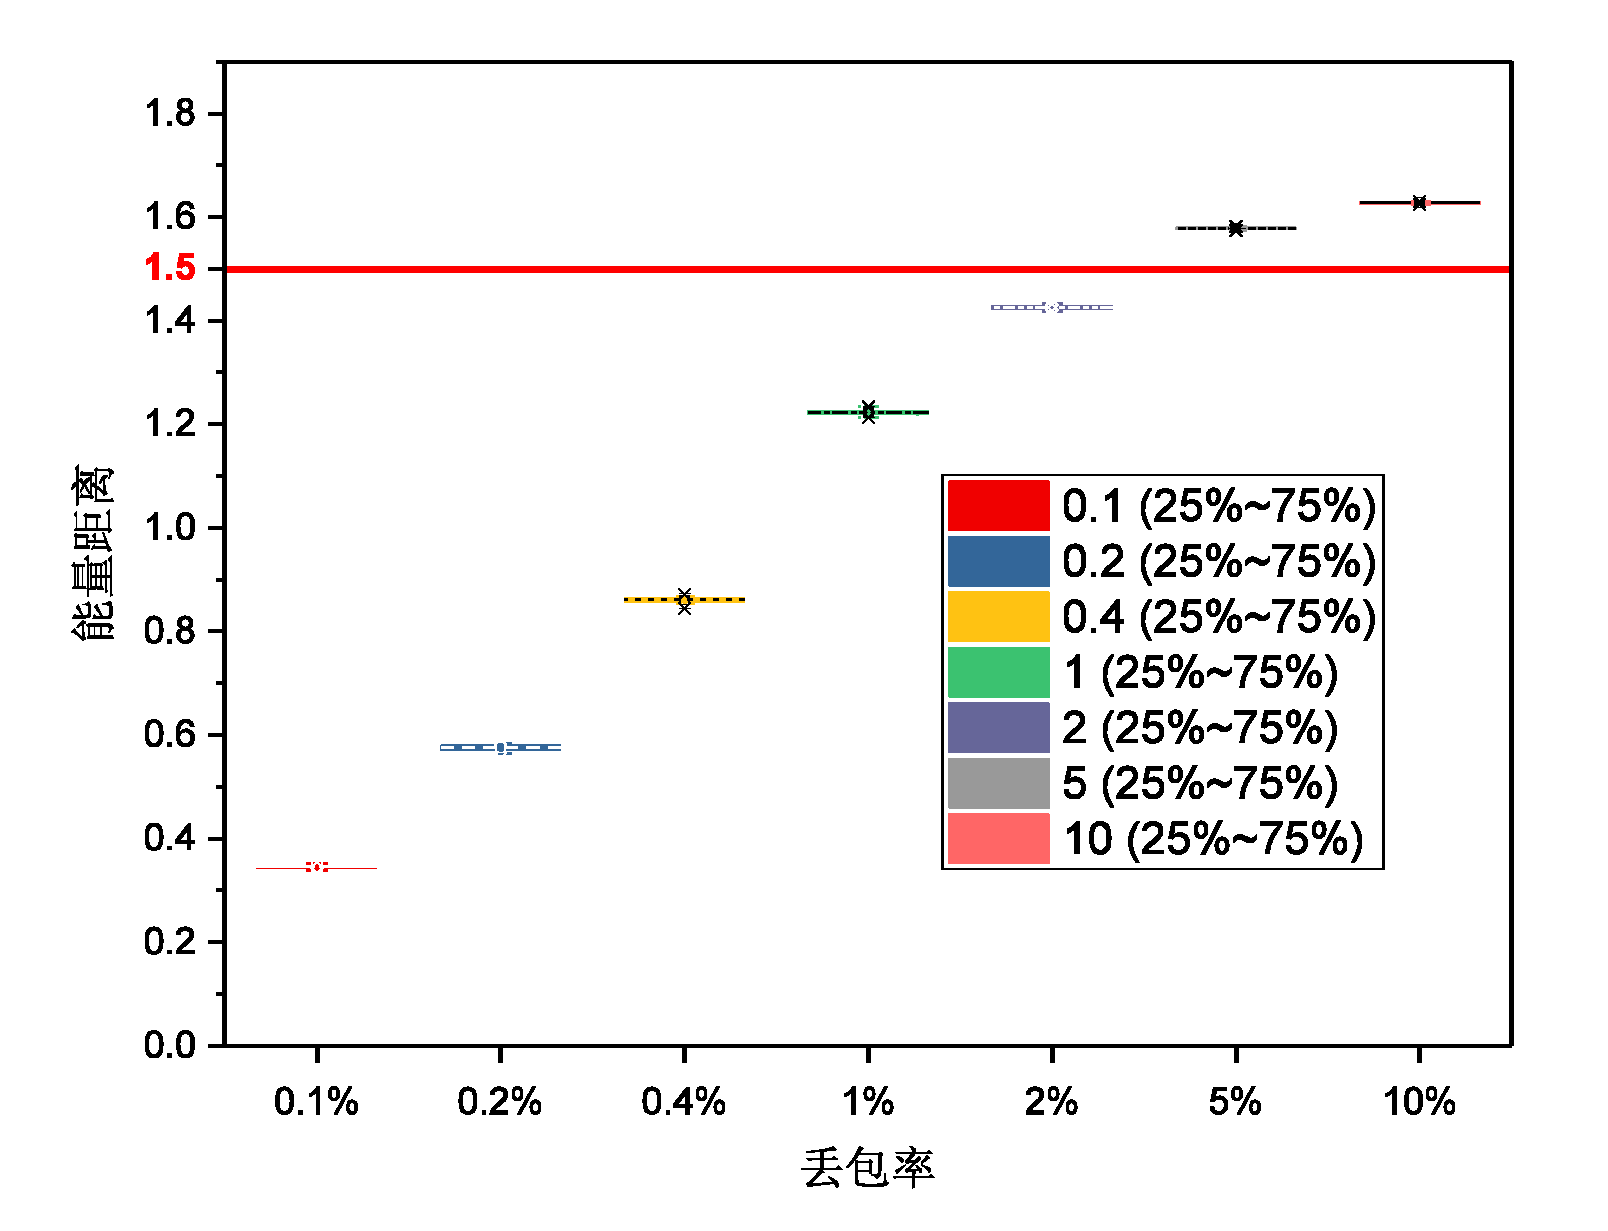
\includegraphics[width=0.48\textwidth]{chapters/chapter3/figures/burst-ed-excellent.pdf}
        }
        \subfigure[Good场景能量距离的箱线图]{
            \label{fig:3:result:burst:ed:good}
            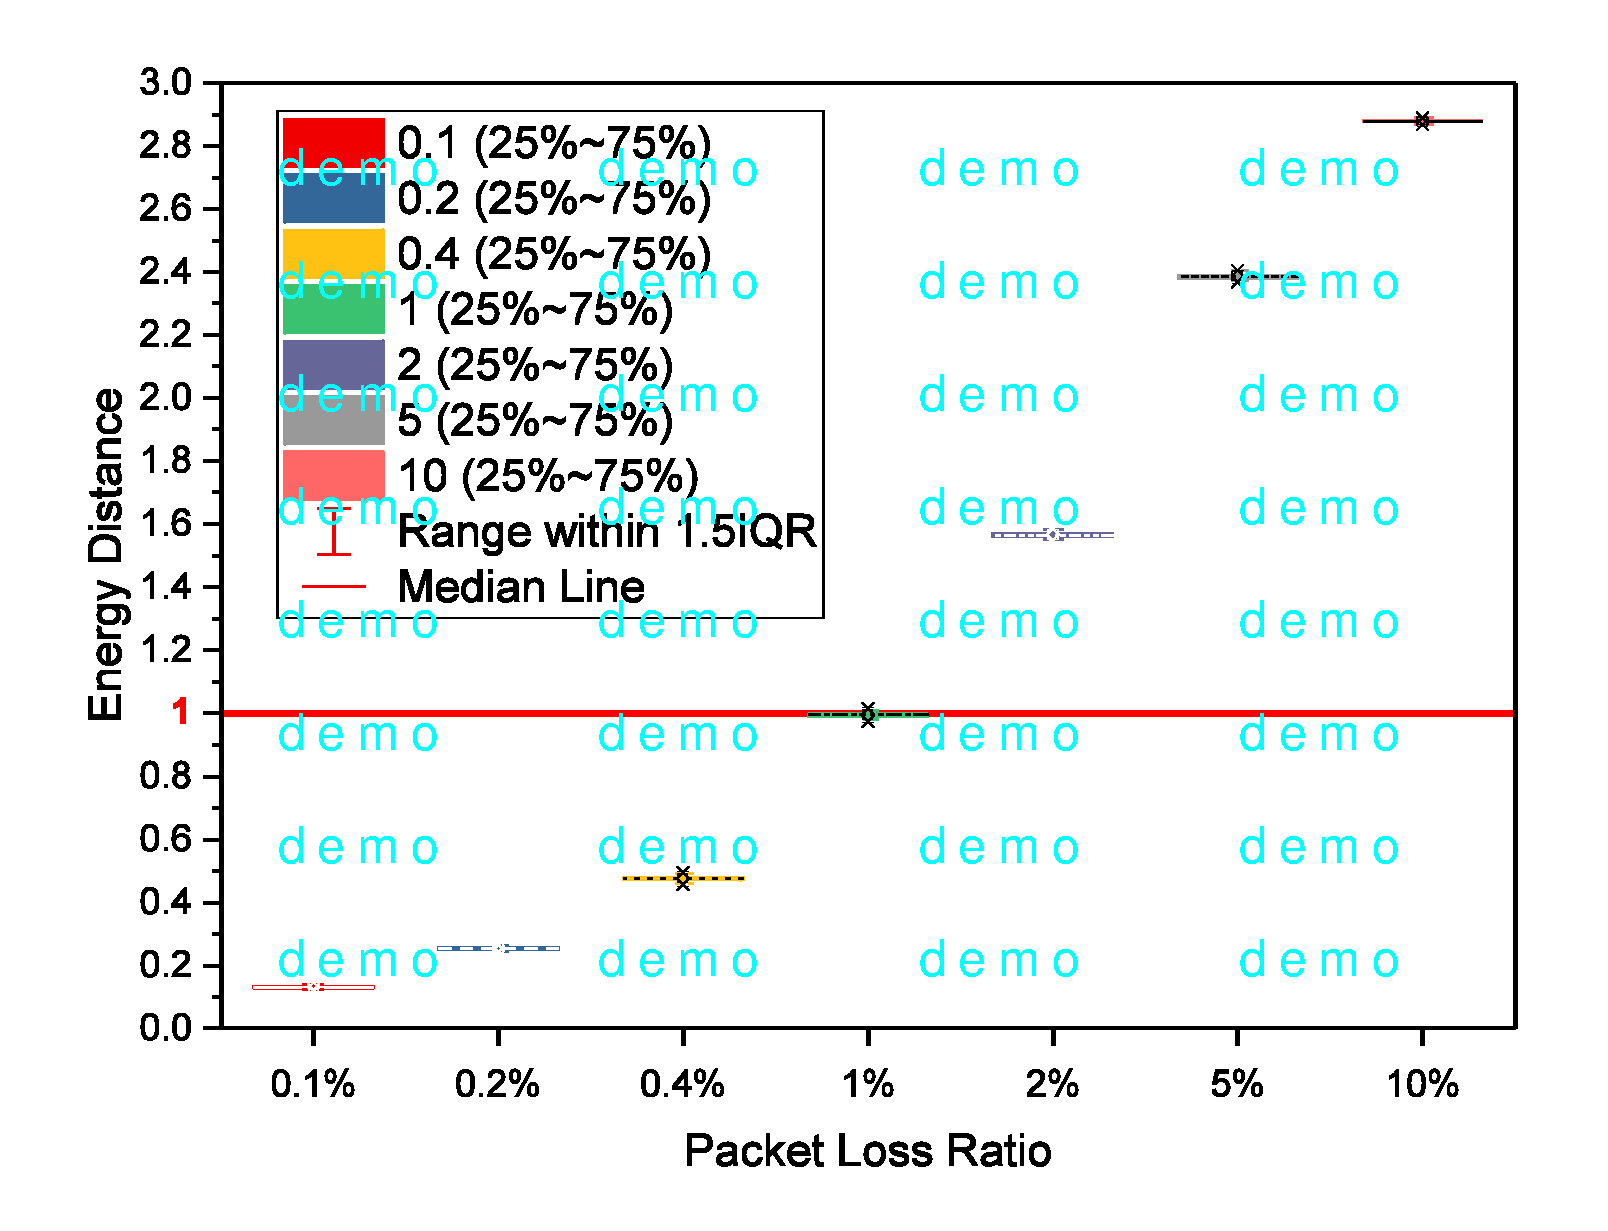
\includegraphics[width=0.48\textwidth]{chapters/chapter3/figures/burst-ed-good.pdf}
        }
        \caption{突发丢包长度能量距离的箱线图}
        \label{fig:3:result:burst:ed}
	\end{figure}
}

\subsubsection{CDF测试结果}
\label{chap:analyze:result:burst:cdf}

如图\nref{fig:3:result:burst:cdf},基于主动丢包的时间隐通道,对突发丢包长度的分布有显著影响。图\nref{fig:3:result:burst:cdf:excellent}Excellent场景中,随着PLR的增加,曲线的上升趋势明显加快,明显偏离原始分布。图\nref{fig:3:result:burst:cdf:good}Good场景中,由于原分布中已经存在较多的丢包,所以构建时间隐通道导致的分布改变较小,但对比原始分布,曲线的上升趋势也明显改变。因此,通过CDF判断,测试样本中存在时间隐通道的可能性,需要进一步量化评估。

\subsubsection{条件熵测试结果}
\label{chap:analyze:result:burst:kld}

如图\nref{fig:3:result:burst:kld},通过K-L散度已经能够明显将时间隐通道检测出来。图\nref{fig:3:result:burst:kld:excellent}中,只有丢包率$\le 0.2\%$时,才可以通过K-L散度检测,说明在良好的网络条件下,通过主动丢包构建时间隐通道要求较高。图\nref{fig:3:result:burst:kld:good}中,可以发现当丢包率$\le 1\%$时,即可通过K-L散度检测,说明在Good场景中,基于主动丢包的时间隐通道,更容易隐蔽于网络噪声中。

\subsubsection{相对距离测试结果}
\label{chap:analyze:result:burst:distance}

如图\nref{fig:3:result:burst:wd},突发丢包长度进行Wasserstein距离测试的结果,两种场景中的总体趋势是一致的。在Excellent场景中,丢包率$\le 10\%$都可以通过Wasserstein距离测试;而在Good场景中,当丢包率$\le 2\%$才可以通过测试。由于时间隐通道产生的突发丢包长度为1,Excellent场景中丢包长度为1的占主要部分,而Good场景中所占比例要小,因此Good场景中的累积结果更加显著。图\nref{fig:3:result:burst:ed},为能量距离的检测结果。Excellent场景下,丢包率$\le 2\%$即可通过检验;Good场景下,丢包率$\le 1\%$才可以通过检验。能量距离检测要求较Wasserstein更加严格,Good场景较Excellent场景更加严格。在相对距离测试中,可以发现最终结果的变化范围非常明显,各种参数下的距离值存在明显的界限,并且检测结果与CDF曲线的相对趋势是一致的。

对比\nref{chap:analyze:result:ipd}中基于IPD的检测结果,基于突发丢包长度分布的测试,已能有效检测基于主动丢包的时间隐通道。在Excellent场景下,由于对丢包比较敏感,K-L散度具有更好的检测效果;在Good场景下,相对距离检测对分布的累积差异更加敏感,检测结果优于Excellent场景。

\subsection{区间丢包数测试结果评估}
\label{chap:analyze:result:window}

如图\nref{fig:3:capture:win-cdf},通过设定不同的窗口长度,窗口区间内的丢包数量的分布,会随之变化。较小的窗口有益于Excellent场景的检测,较大的窗口有益于Good场景的检测。在本测试中,选取窗口长度100和200两种。

\insertFigure{
	\begin{figure}
        \centering
        \subfigure[窗口100时Excellent场景的CDF]{
            \label{fig:3:result:win100:cdf:excellent}
            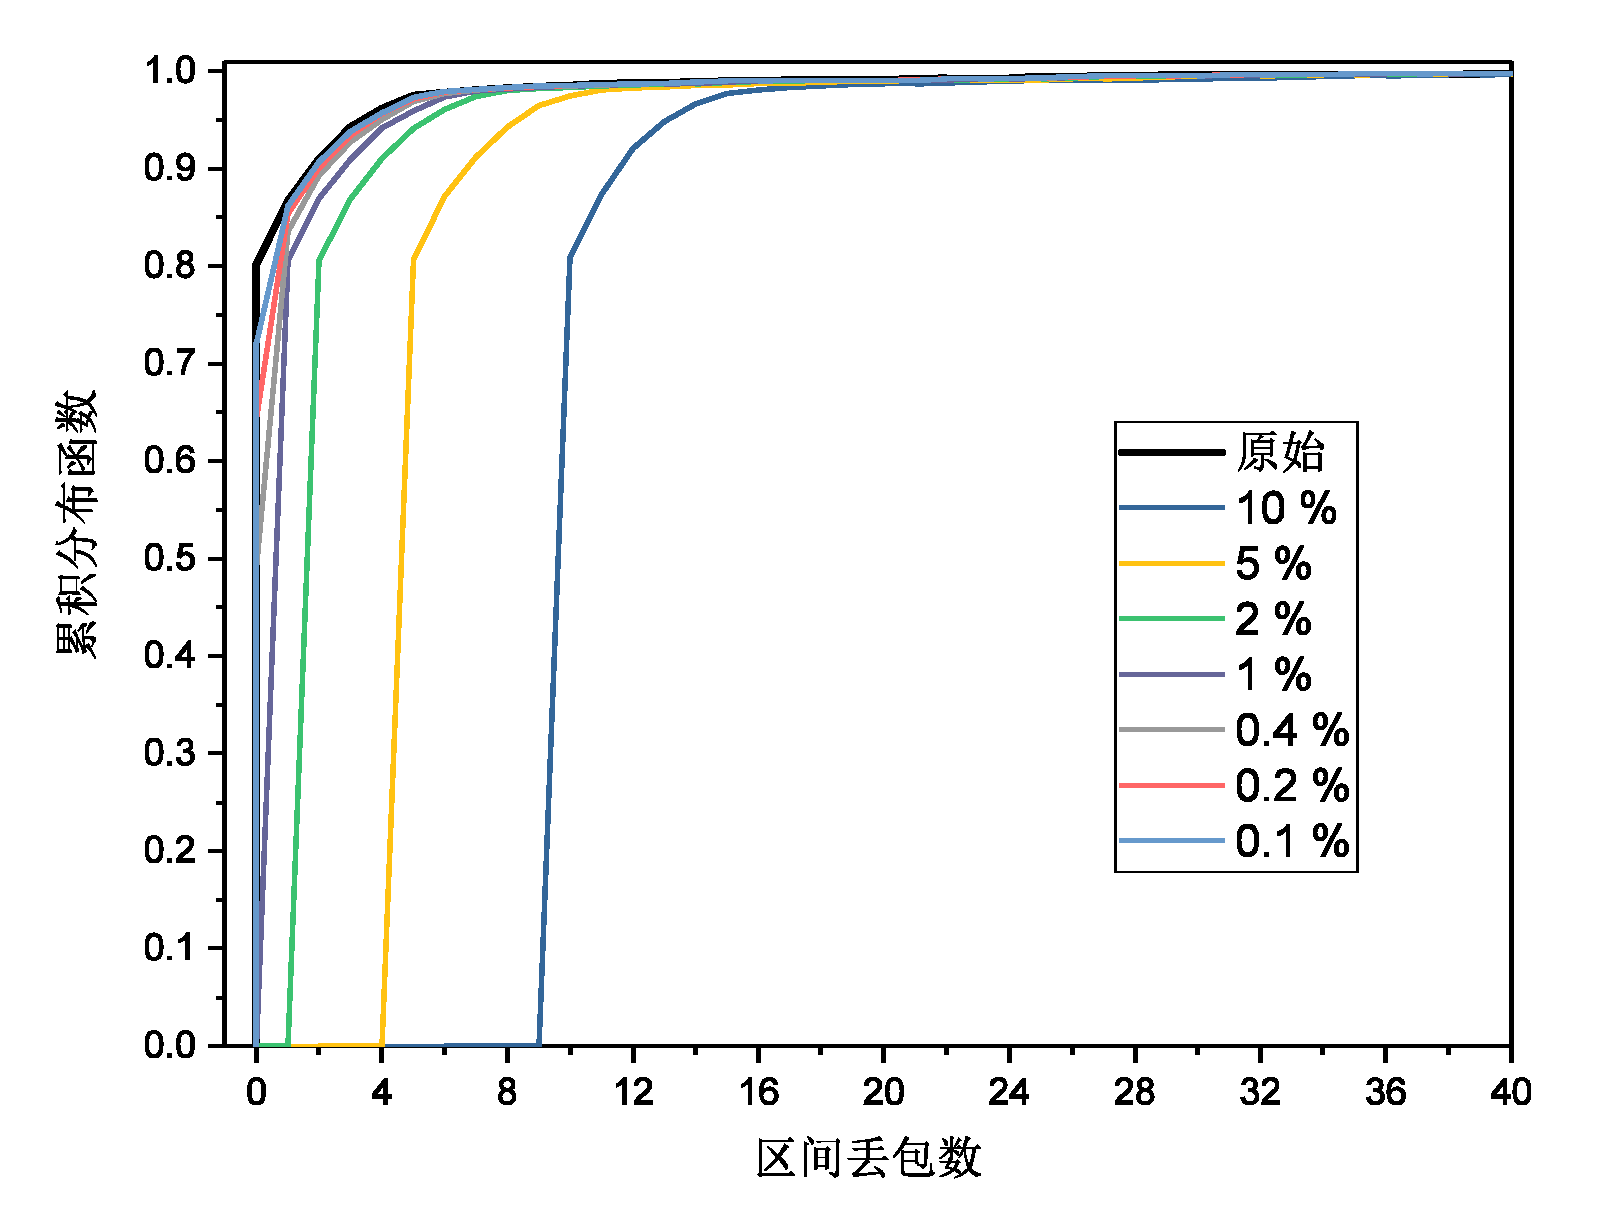
\includegraphics[width=0.48\textwidth]{chapters/chapter3/figures/win100-cdf-excellent.pdf}
        }
        \subfigure[窗口100时Good场景的CDF]{
            \label{fig:3:result:win100:cdf:good}
            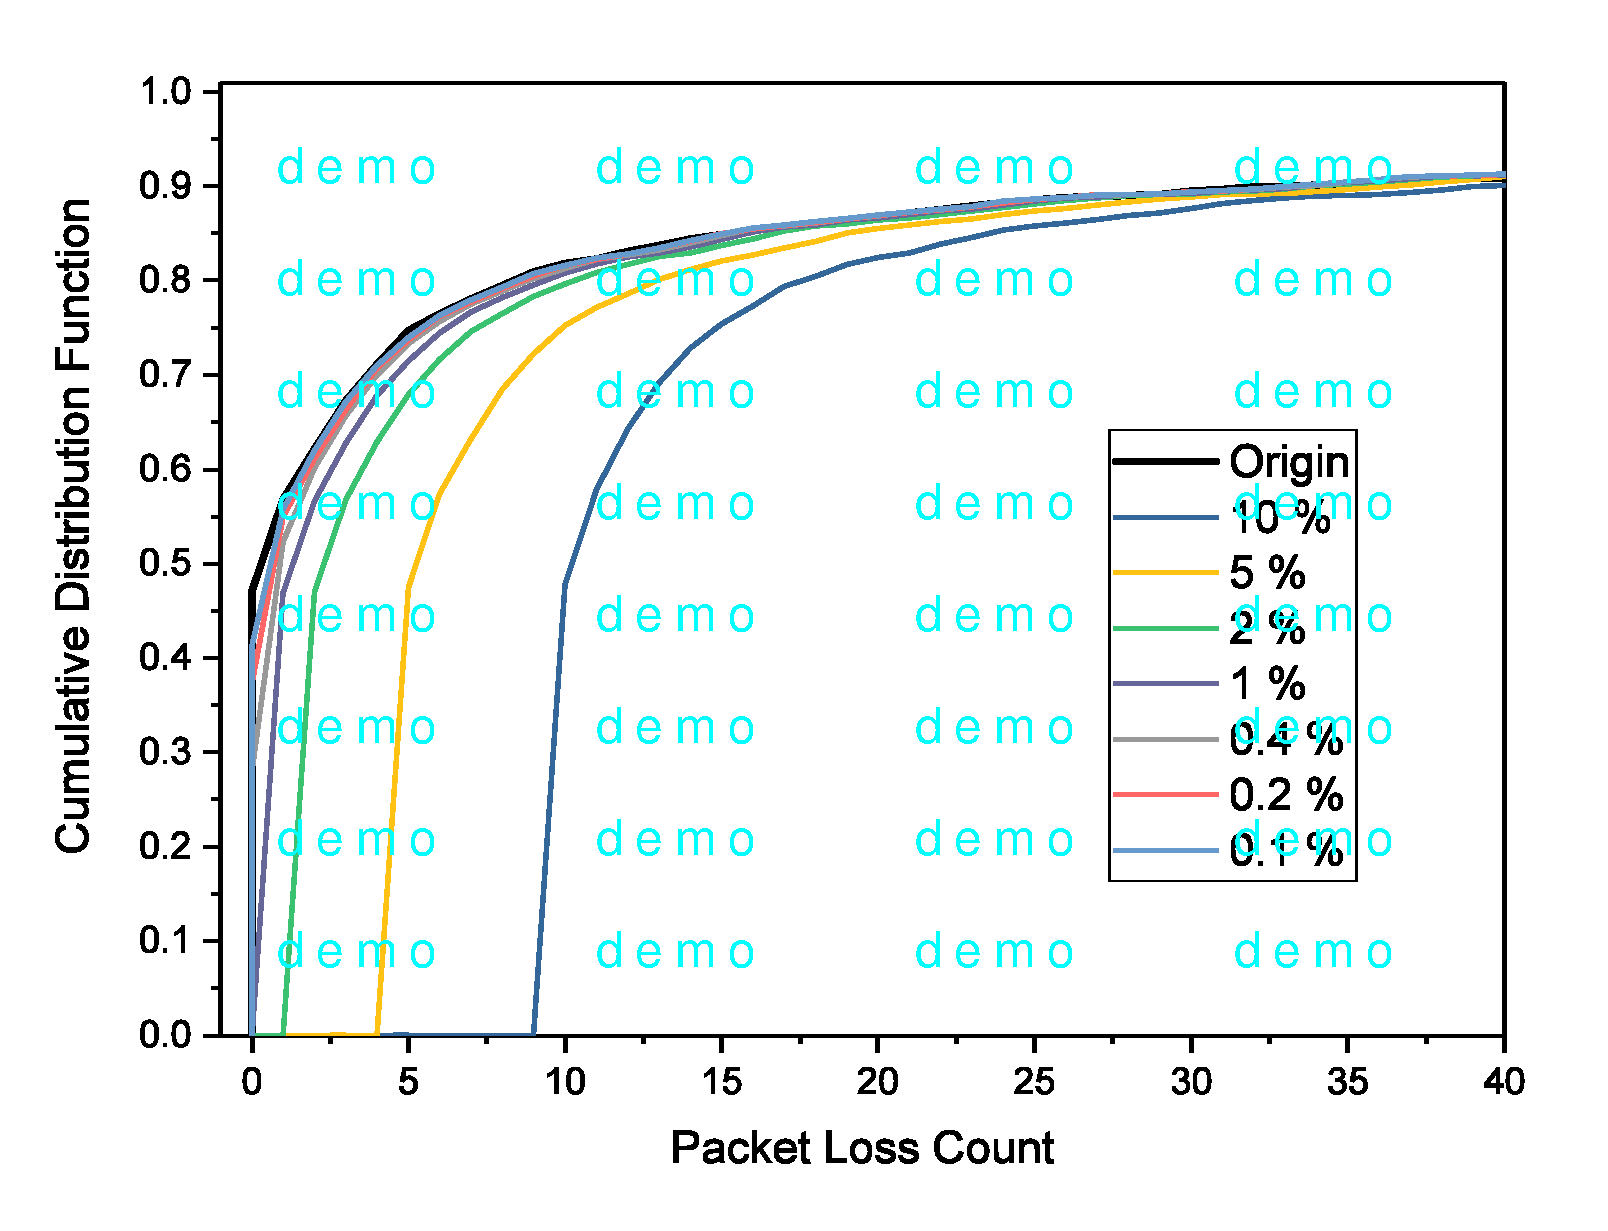
\includegraphics[width=0.48\textwidth]{chapters/chapter3/figures/win100-cdf-good.pdf}
        }
        \subfigure[窗口200时Excellent场景的CDF]{
            \label{fig:3:result:win200:cdf:excellent}
            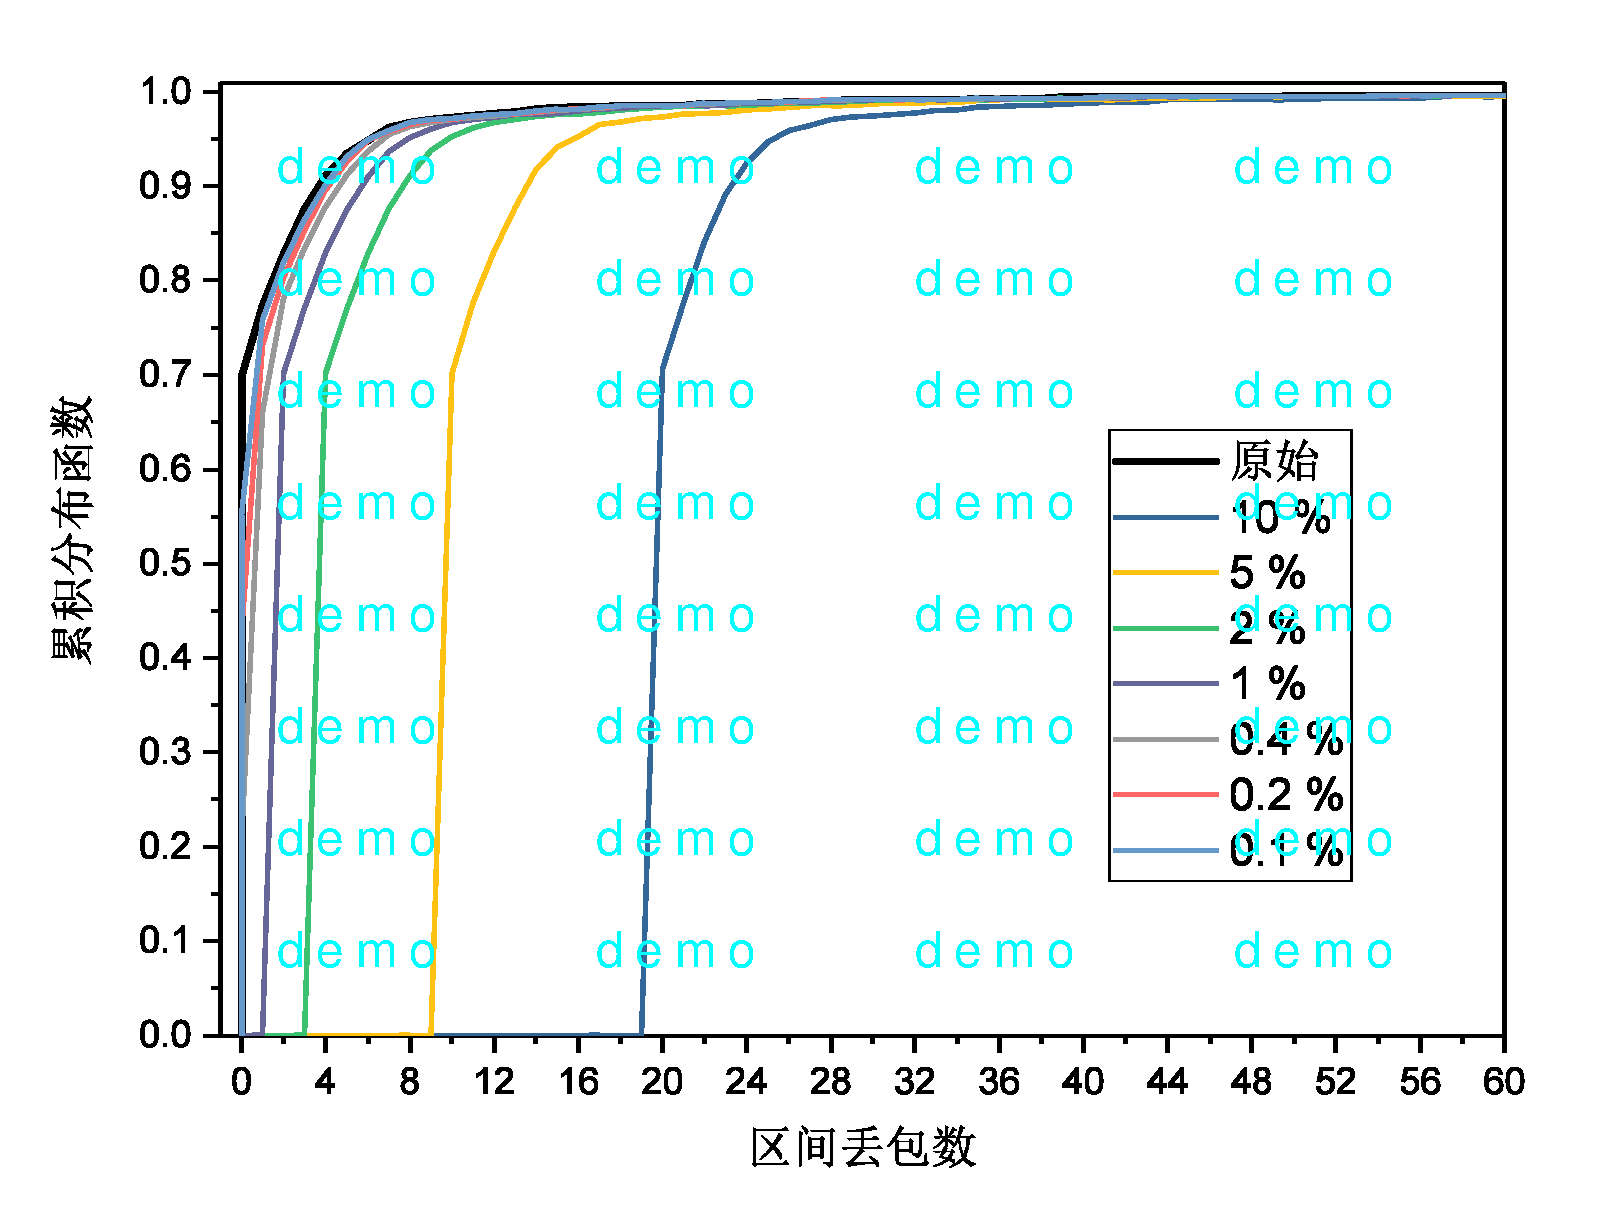
\includegraphics[width=0.48\textwidth]{chapters/chapter3/figures/win200-cdf-excellent.pdf}
        }
        \subfigure[窗口200时Good场景的CDF]{
            \label{fig:3:result:win200:cdf:good}
            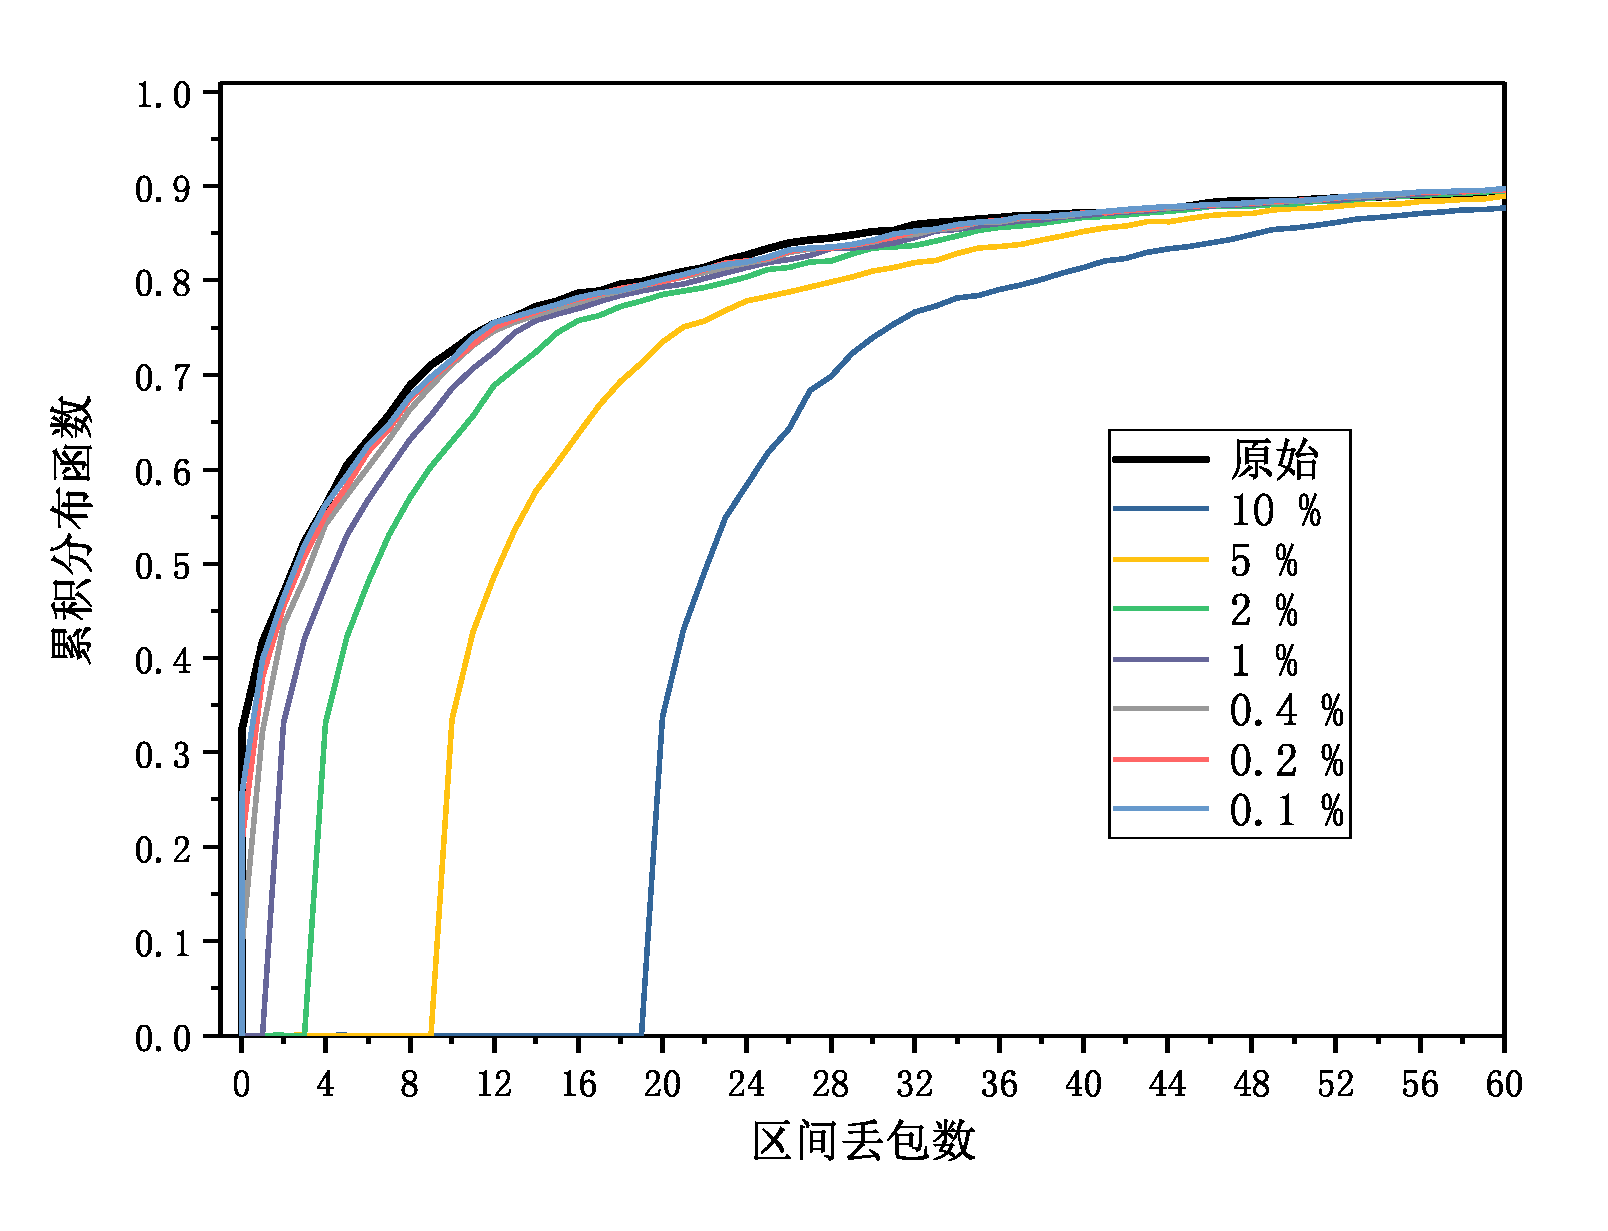
\includegraphics[width=0.48\textwidth]{chapters/chapter3/figures/win200-cdf-good.pdf}
        }
        \caption{区间丢包数的CDF曲线}
        \label{fig:3:result:win:cdf}
	\end{figure}
}

\insertFigure{
	\begin{figure}
        \centering
        \subfigure[窗口100时Excellent场景的K-L散度]{
            \label{fig:3:result:win100:kld:excellent}
            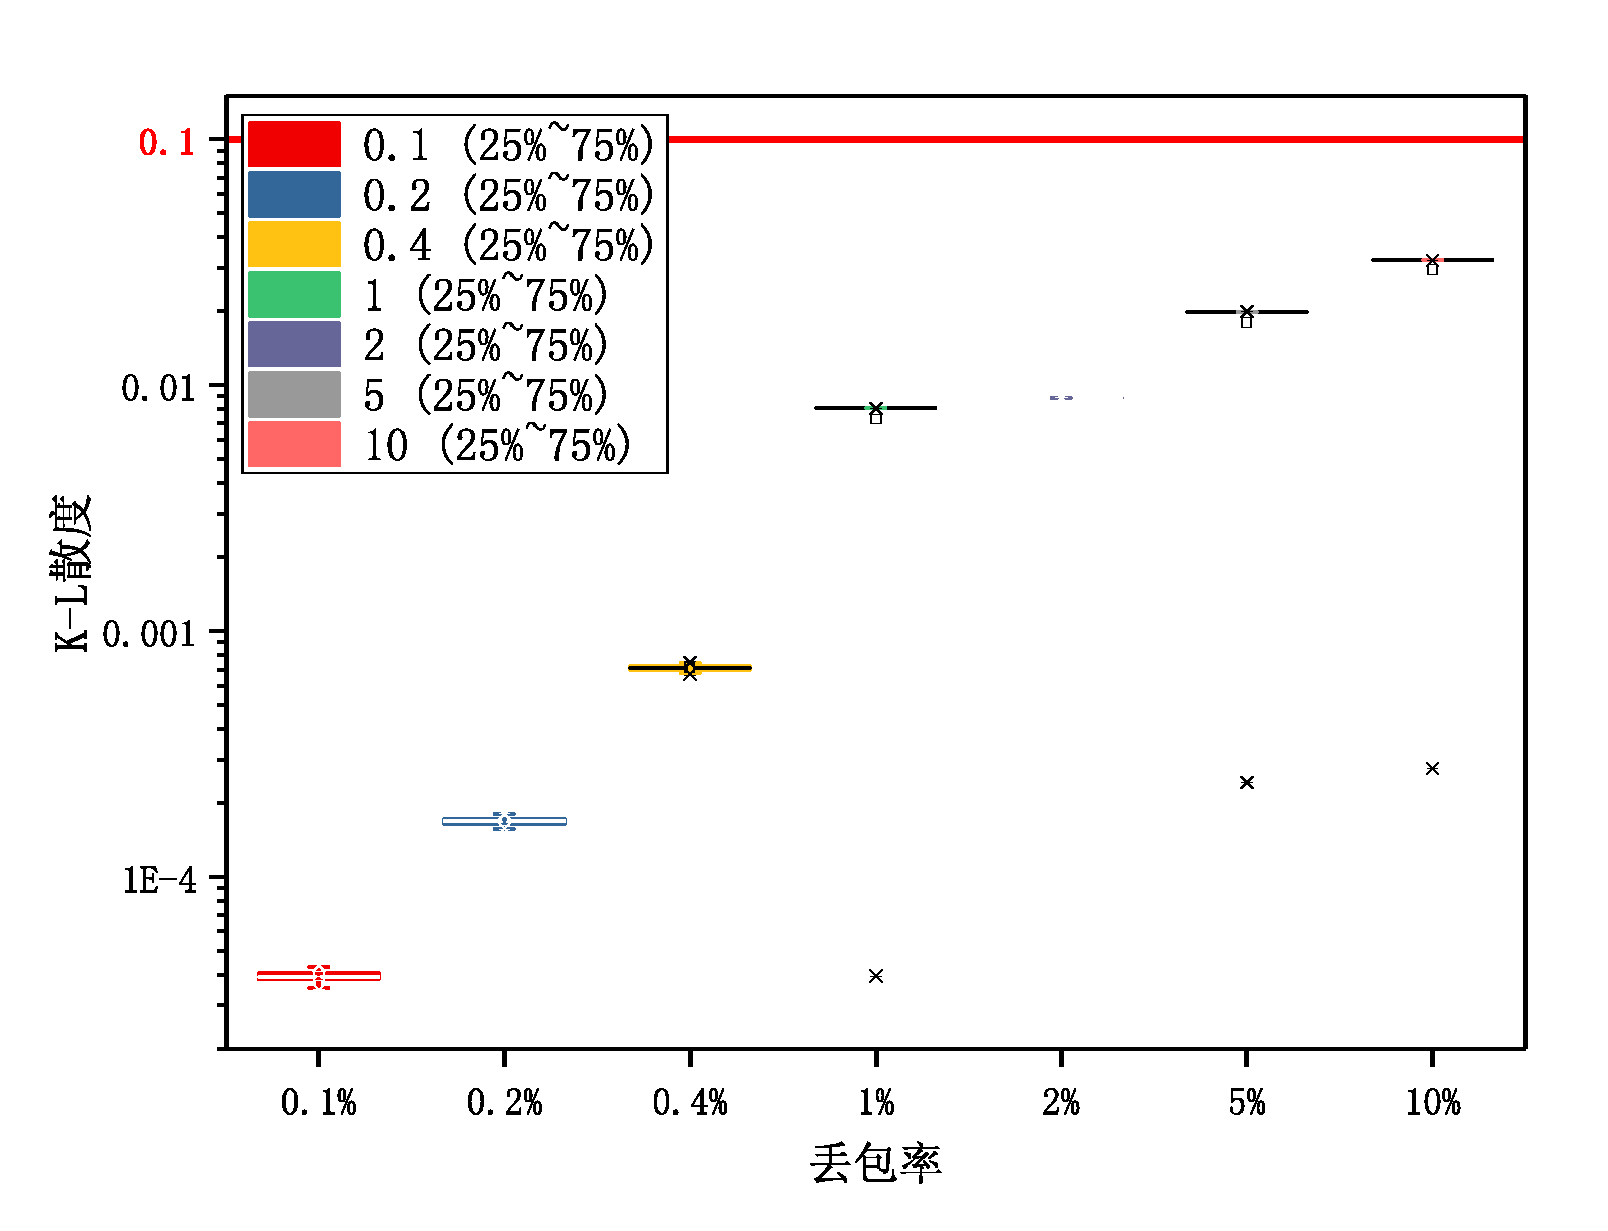
\includegraphics[width=0.48\textwidth]{chapters/chapter3/figures/win100-kld-excellent.pdf}
        }
        \subfigure[窗口100时Good场景的K-L散度]{
            \label{fig:3:result:win100-kld:good}
            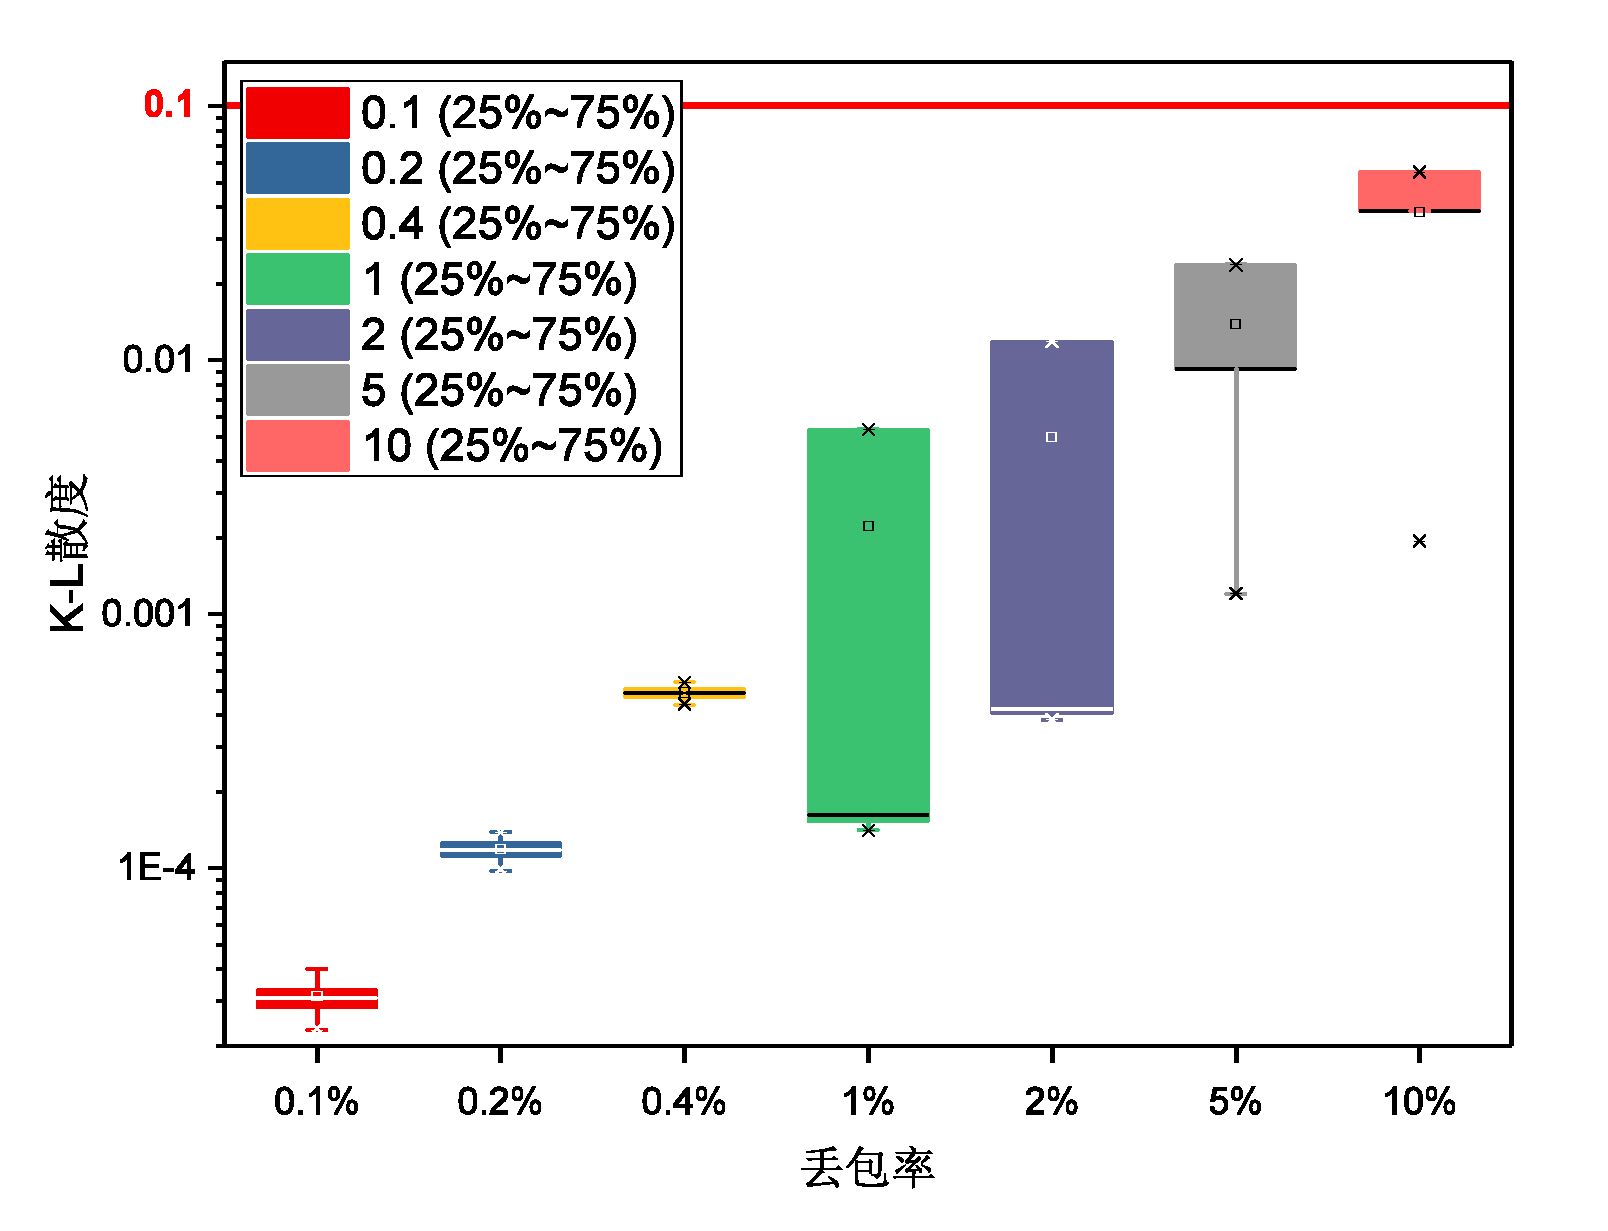
\includegraphics[width=0.48\textwidth]{chapters/chapter3/figures/win100-kld-good.pdf}
        }
        \subfigure[窗口200时Excellent场景的K-L散度]{
            \label{fig:3:result:win200:kld:excellent}
            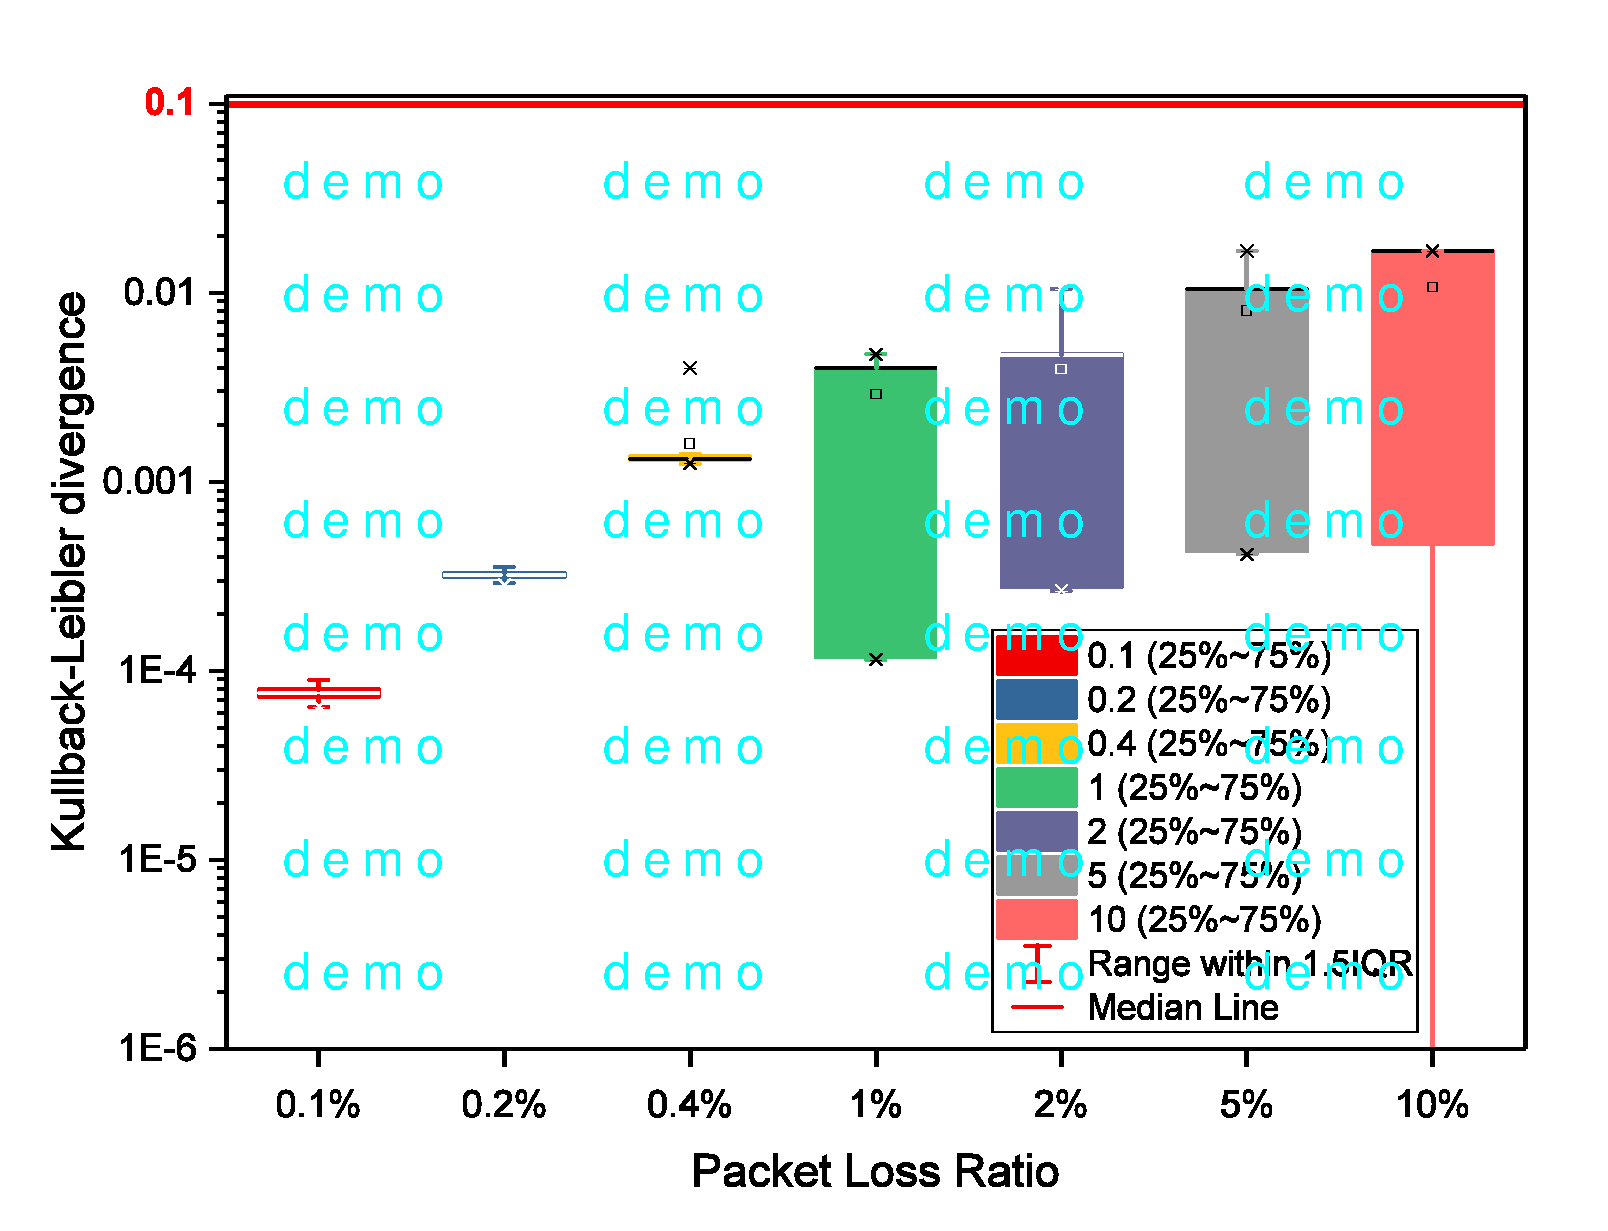
\includegraphics[width=0.48\textwidth]{chapters/chapter3/figures/win200-kld-excellent.pdf}
        }
        \subfigure[窗口200时Good场景的K-L散度]{
            \label{fig:3:result:win200:kld:good}
            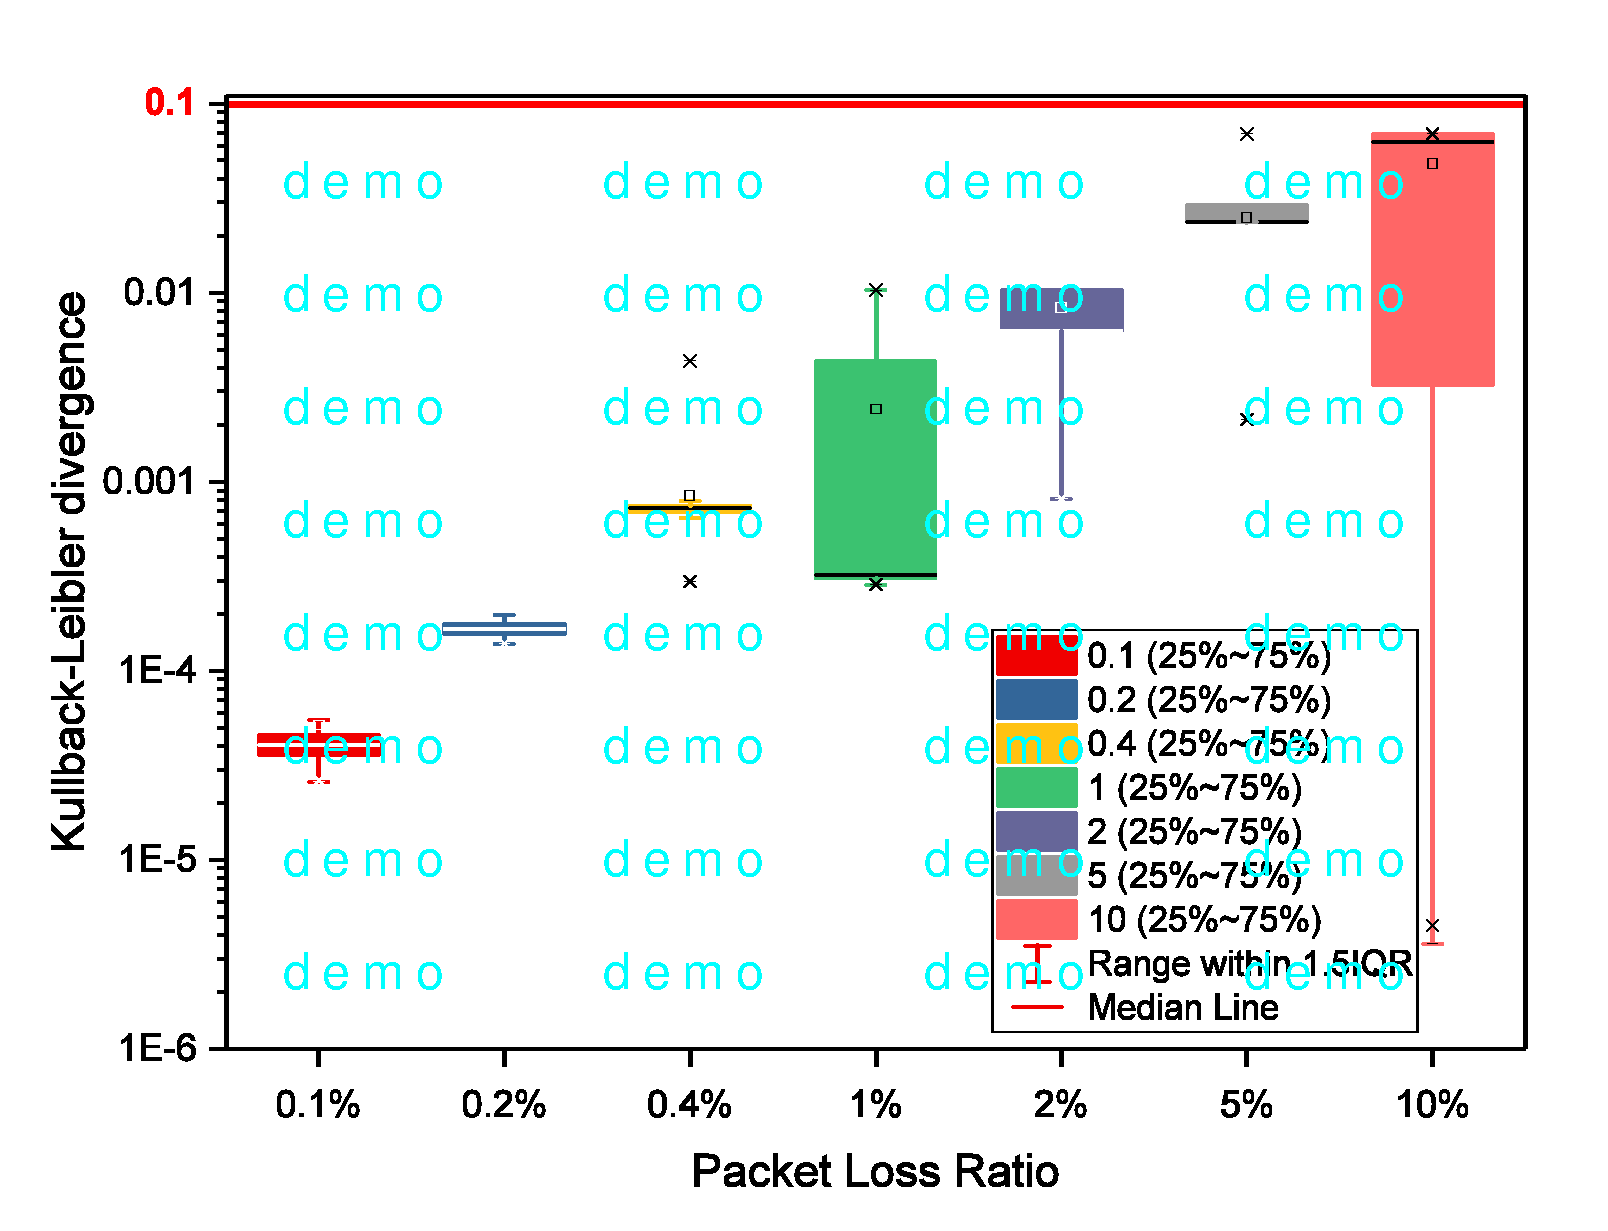
\includegraphics[width=0.48\textwidth]{chapters/chapter3/figures/win200-kld-good.pdf}
        }
        \caption{区间丢包数K-L散度测试的箱线图}
        \label{fig:3:result:win:kld}
	\end{figure}
}

\insertFigure{
	\begin{figure}
        \centering
        \subfigure[窗口100时Excellent场景Wasserstein距离的箱线图]{
            \label{fig:3:result:win100:wd:excellent}
            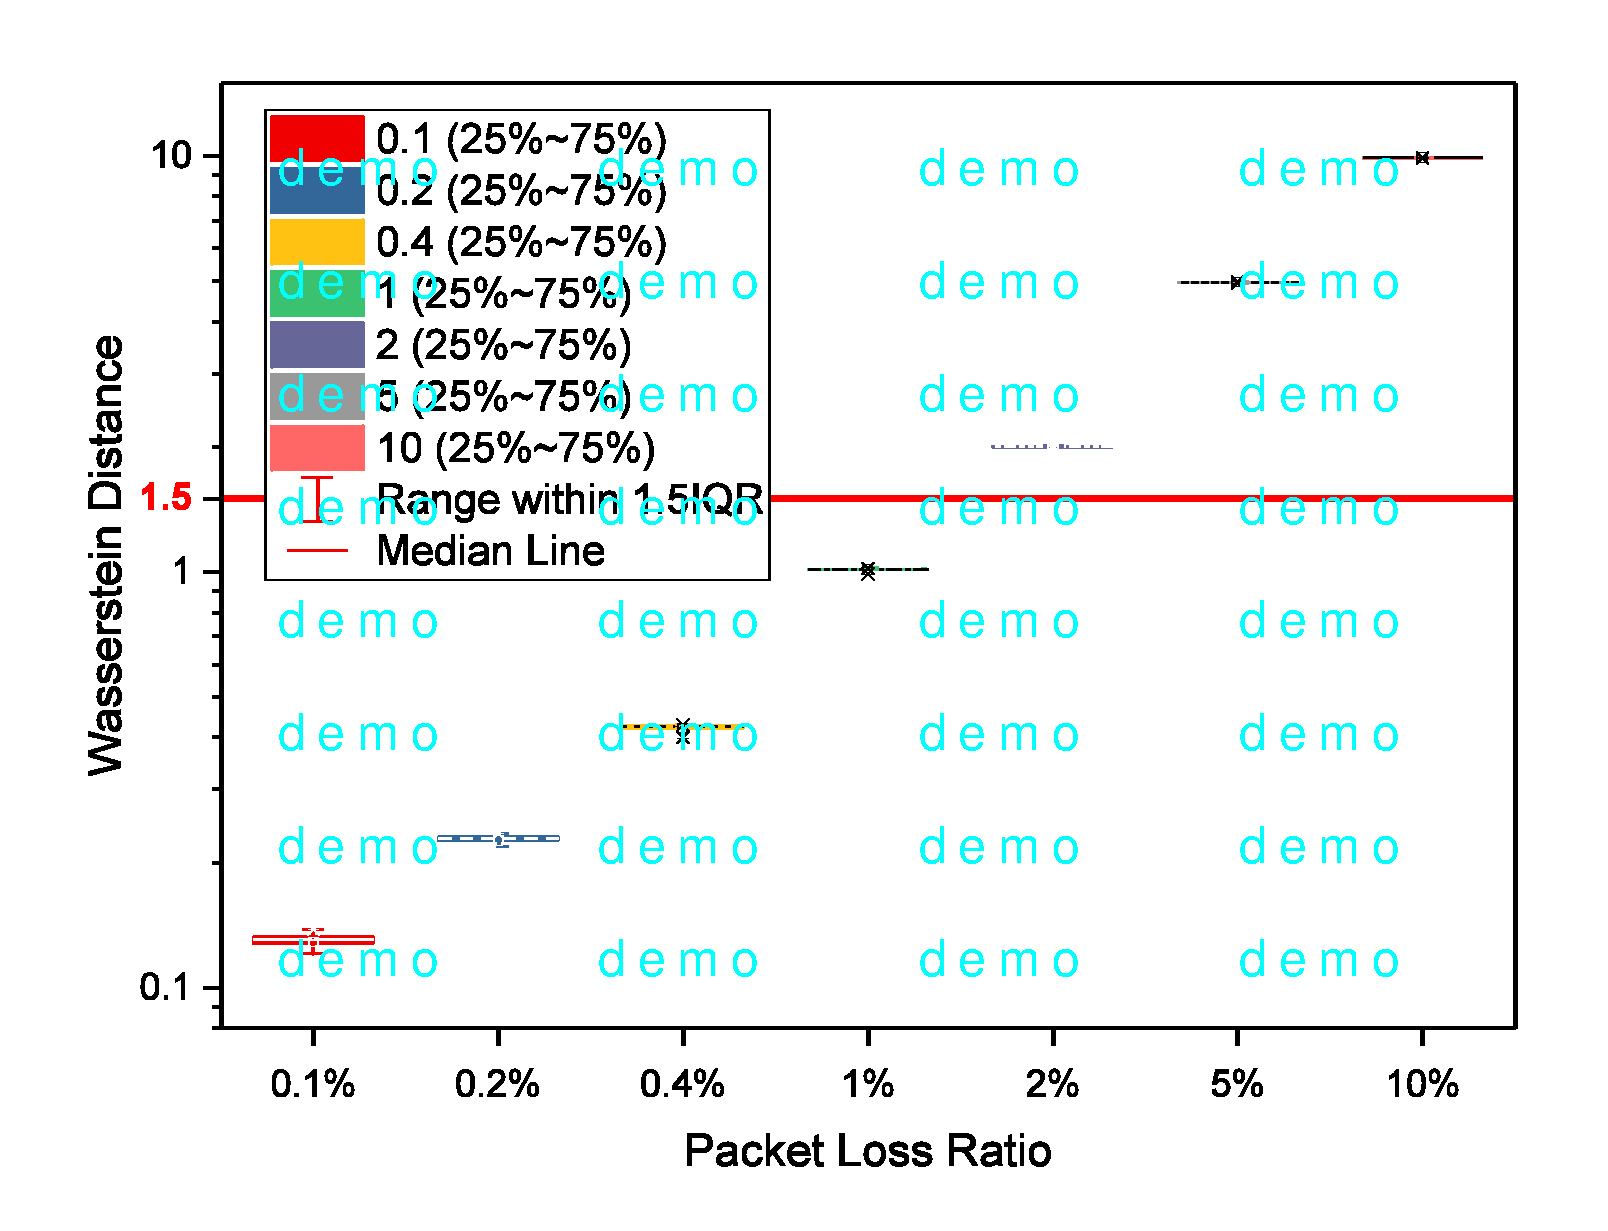
\includegraphics[width=0.48\textwidth]{chapters/chapter3/figures/win100-wd-excellent.pdf}
        }
        \subfigure[窗口100时Good场景Wasserstein距离的箱线图]{
            \label{fig:3:result:win100-wd:good}
            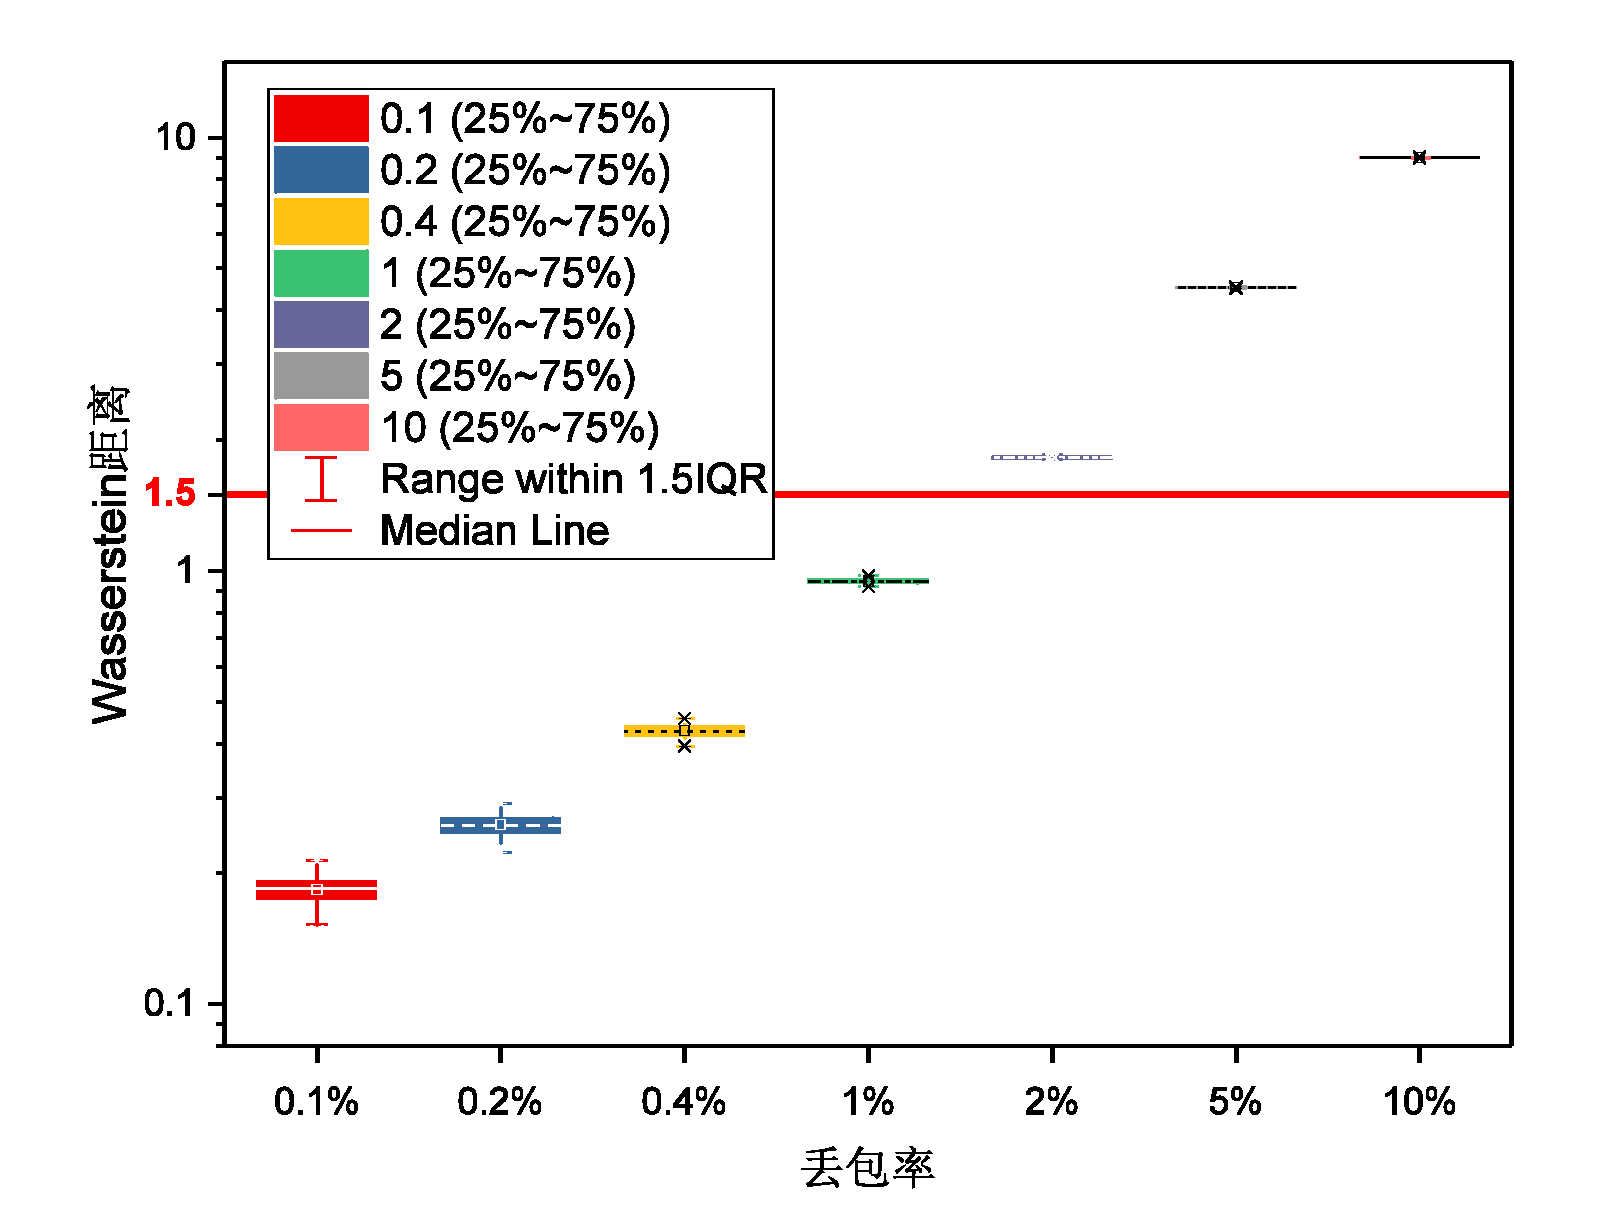
\includegraphics[width=0.48\textwidth]{chapters/chapter3/figures/win100-wd-good.pdf}
        }
        \subfigure[窗口200时Excellent场景Wasserstein距离的箱线图]{
            \label{fig:3:result:win200:wd:excellent}
            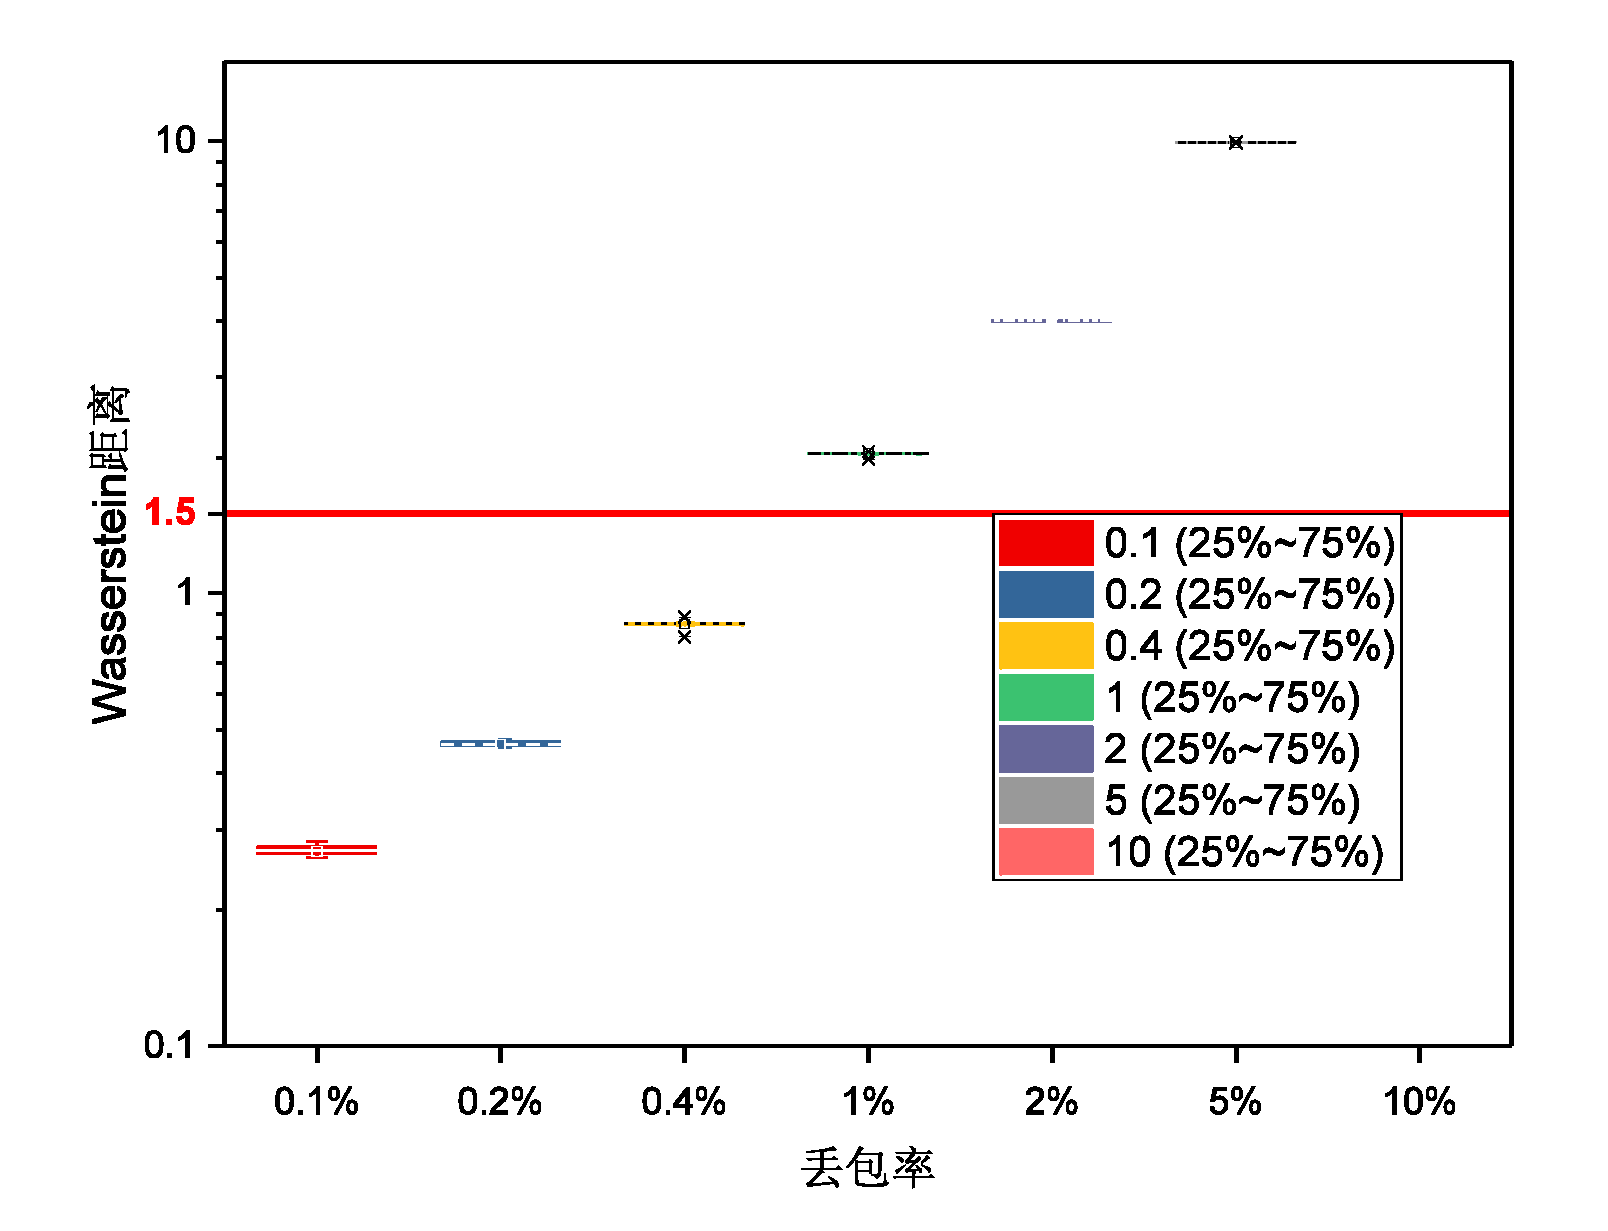
\includegraphics[width=0.48\textwidth]{chapters/chapter3/figures/win200-wd-excellent.pdf}
        }
        \subfigure[窗口200时Good场景Wasserstein距离的箱线图]{
            \label{fig:3:result:win200:wd:good}
            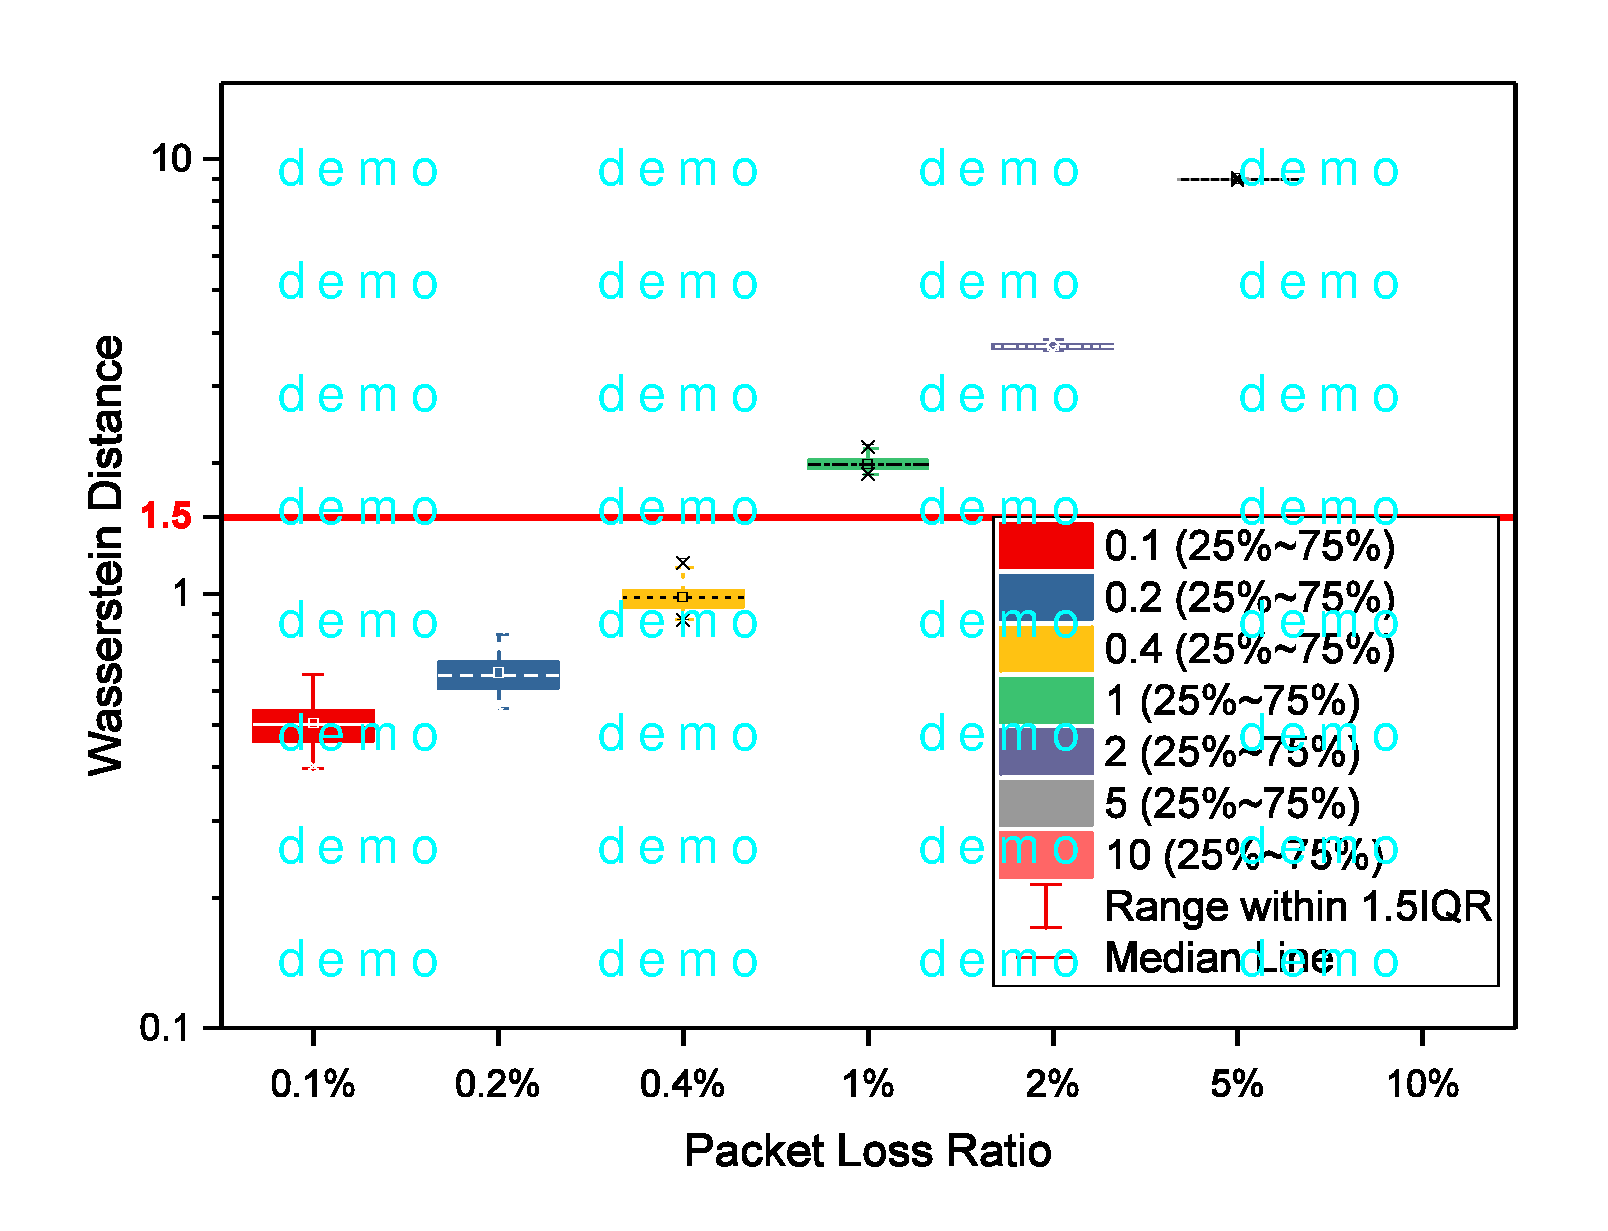
\includegraphics[width=0.48\textwidth]{chapters/chapter3/figures/win200-wd-good.pdf}
        }
        \caption{区间丢包数Wasserstein距离的箱线图}
        \label{fig:3:result:win:wd}
	\end{figure}
}

\insertFigure{
	\begin{figure}
        \centering
        \subfigure[窗口100时Excellent场景能量距离的箱线图]{
            \label{fig:3:result:win100:ed:excellent}
            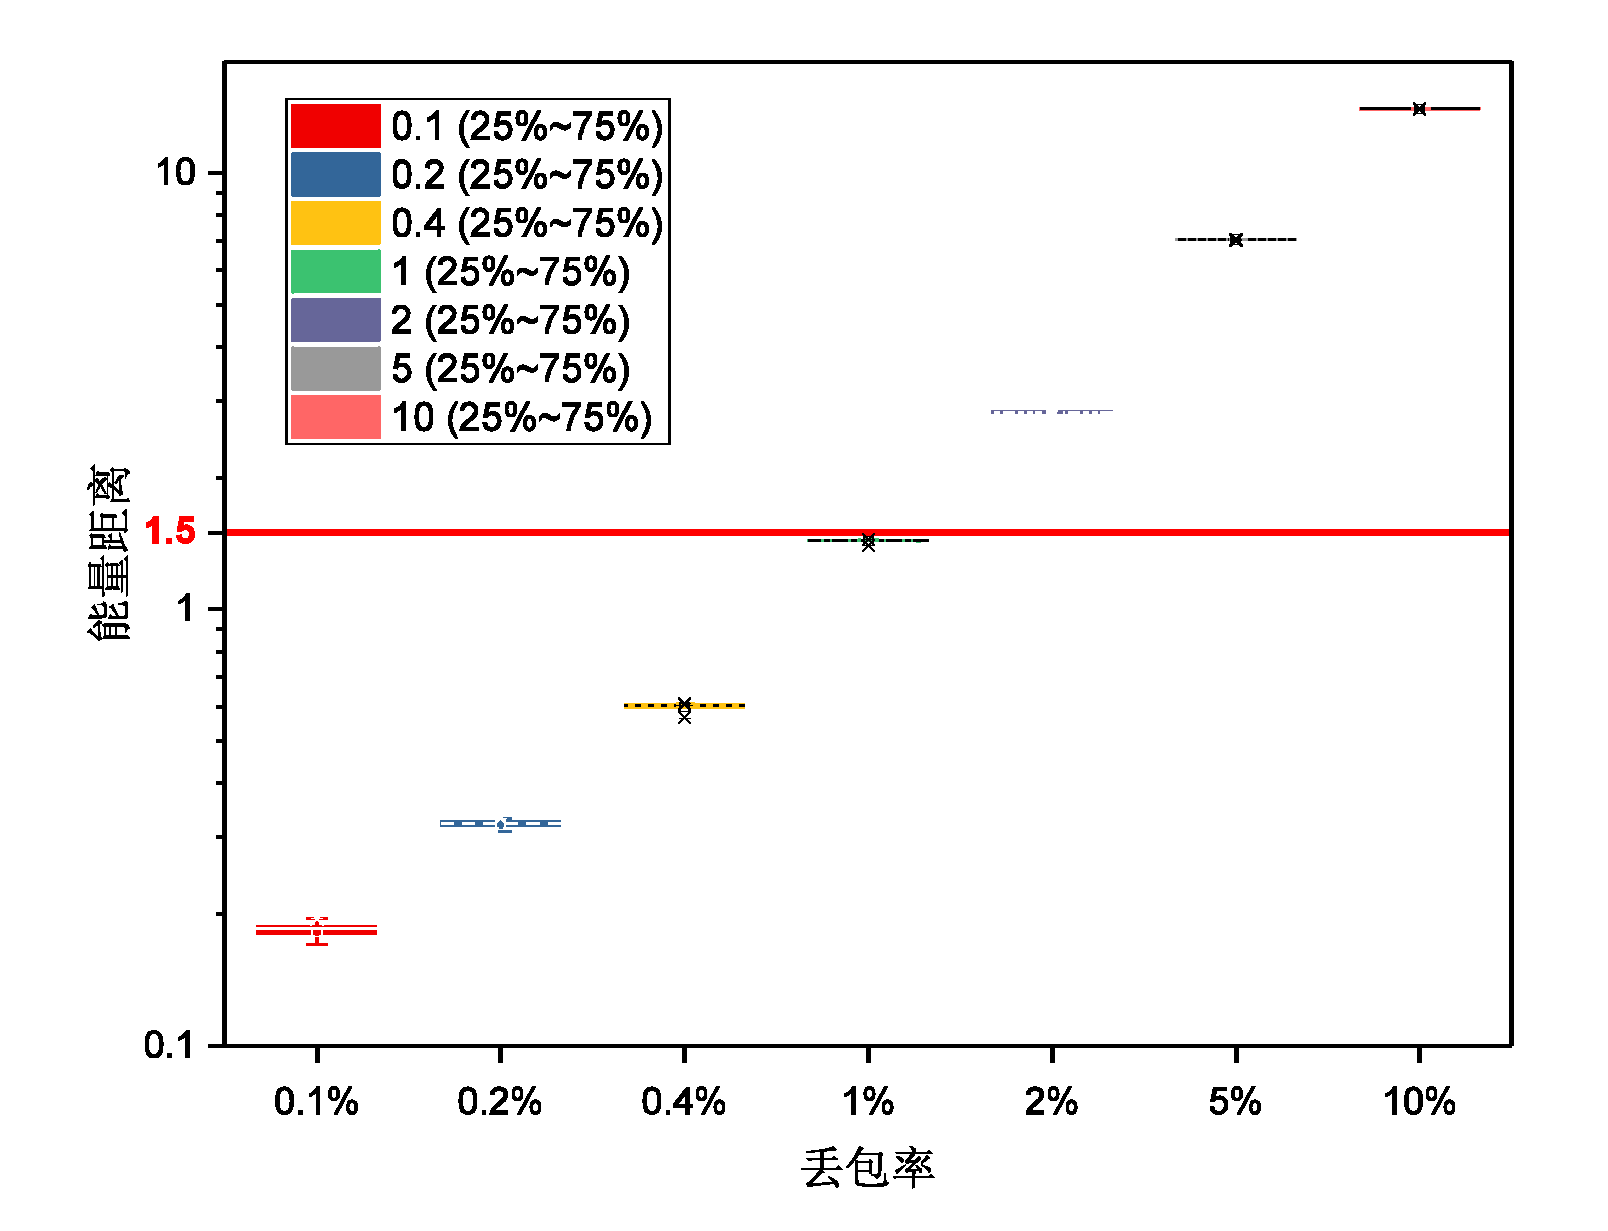
\includegraphics[width=0.48\textwidth]{chapters/chapter3/figures/win100-ed-excellent.pdf}
        }
        \subfigure[窗口100时Good场景能量距离的箱线图]{
            \label{fig:3:result:win100-ed:good}
            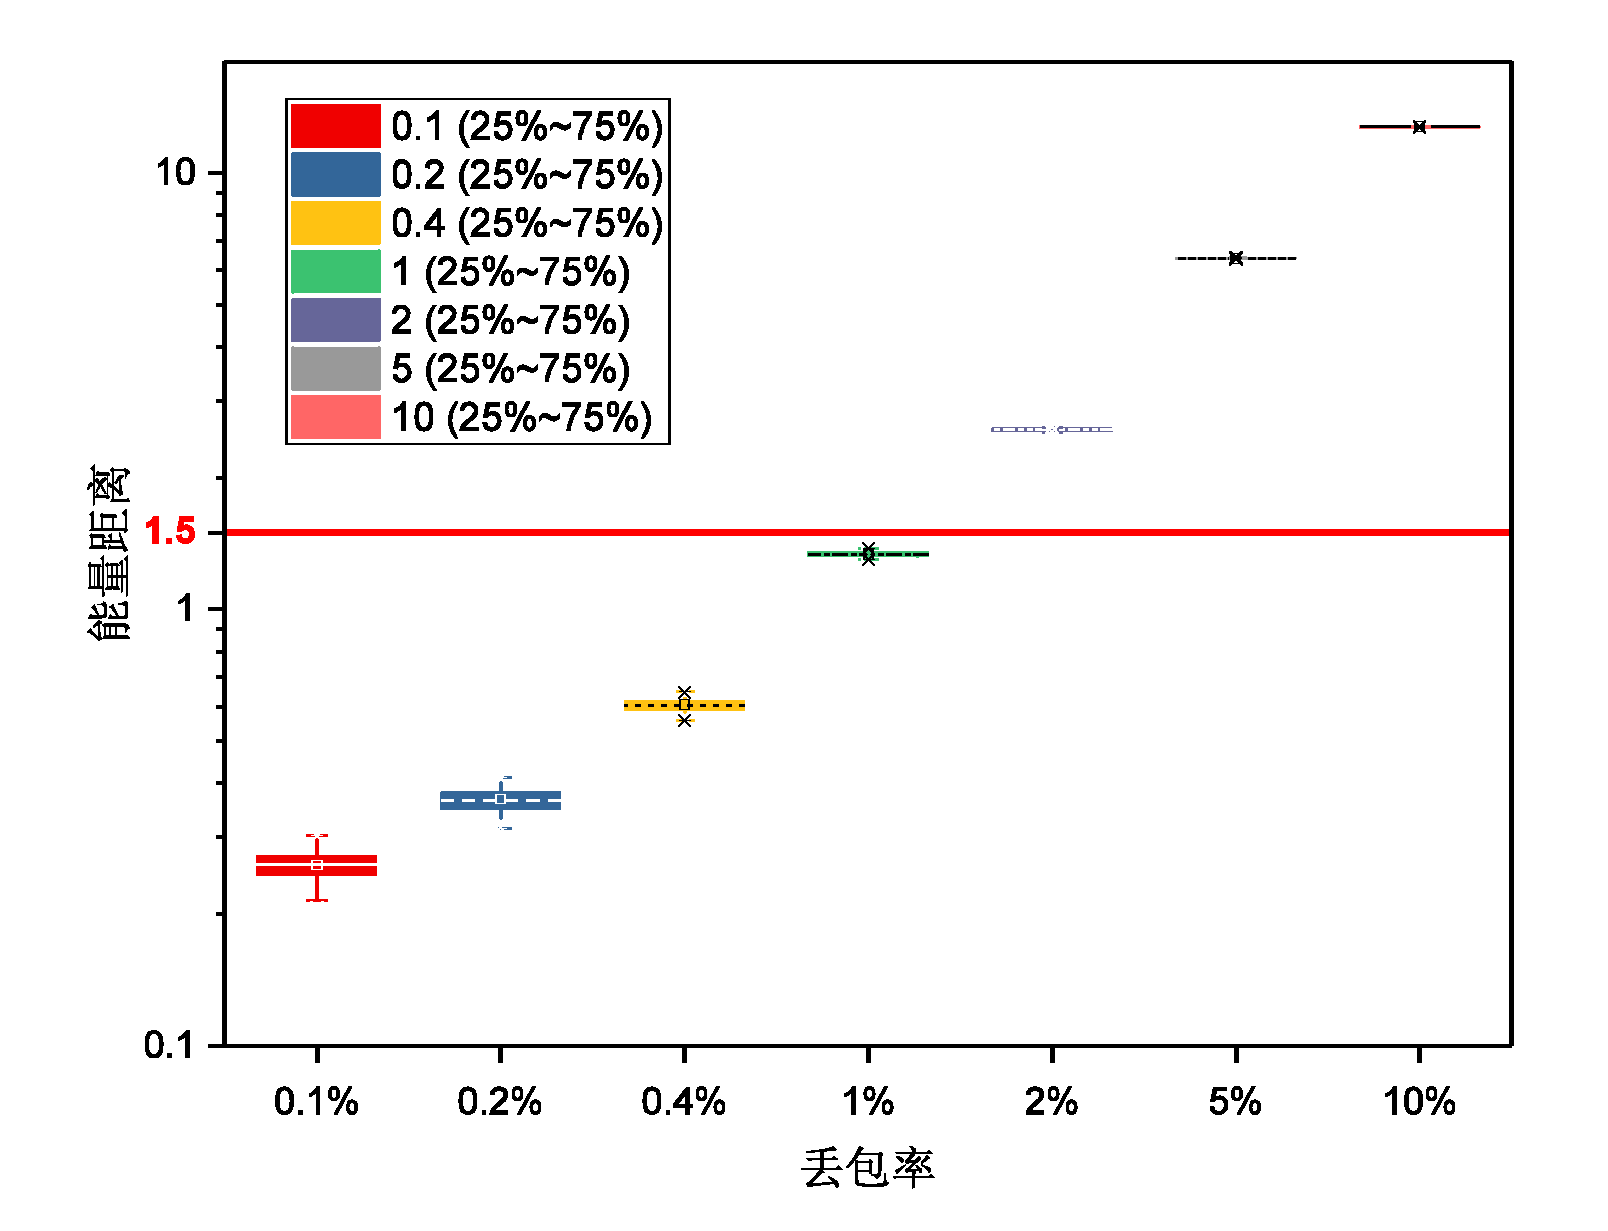
\includegraphics[width=0.48\textwidth]{chapters/chapter3/figures/win100-ed-good.pdf}
        }
        \subfigure[窗口200时Excellent场景能量距离的箱线图]{
            \label{fig:3:result:win200:ed:excellent}
            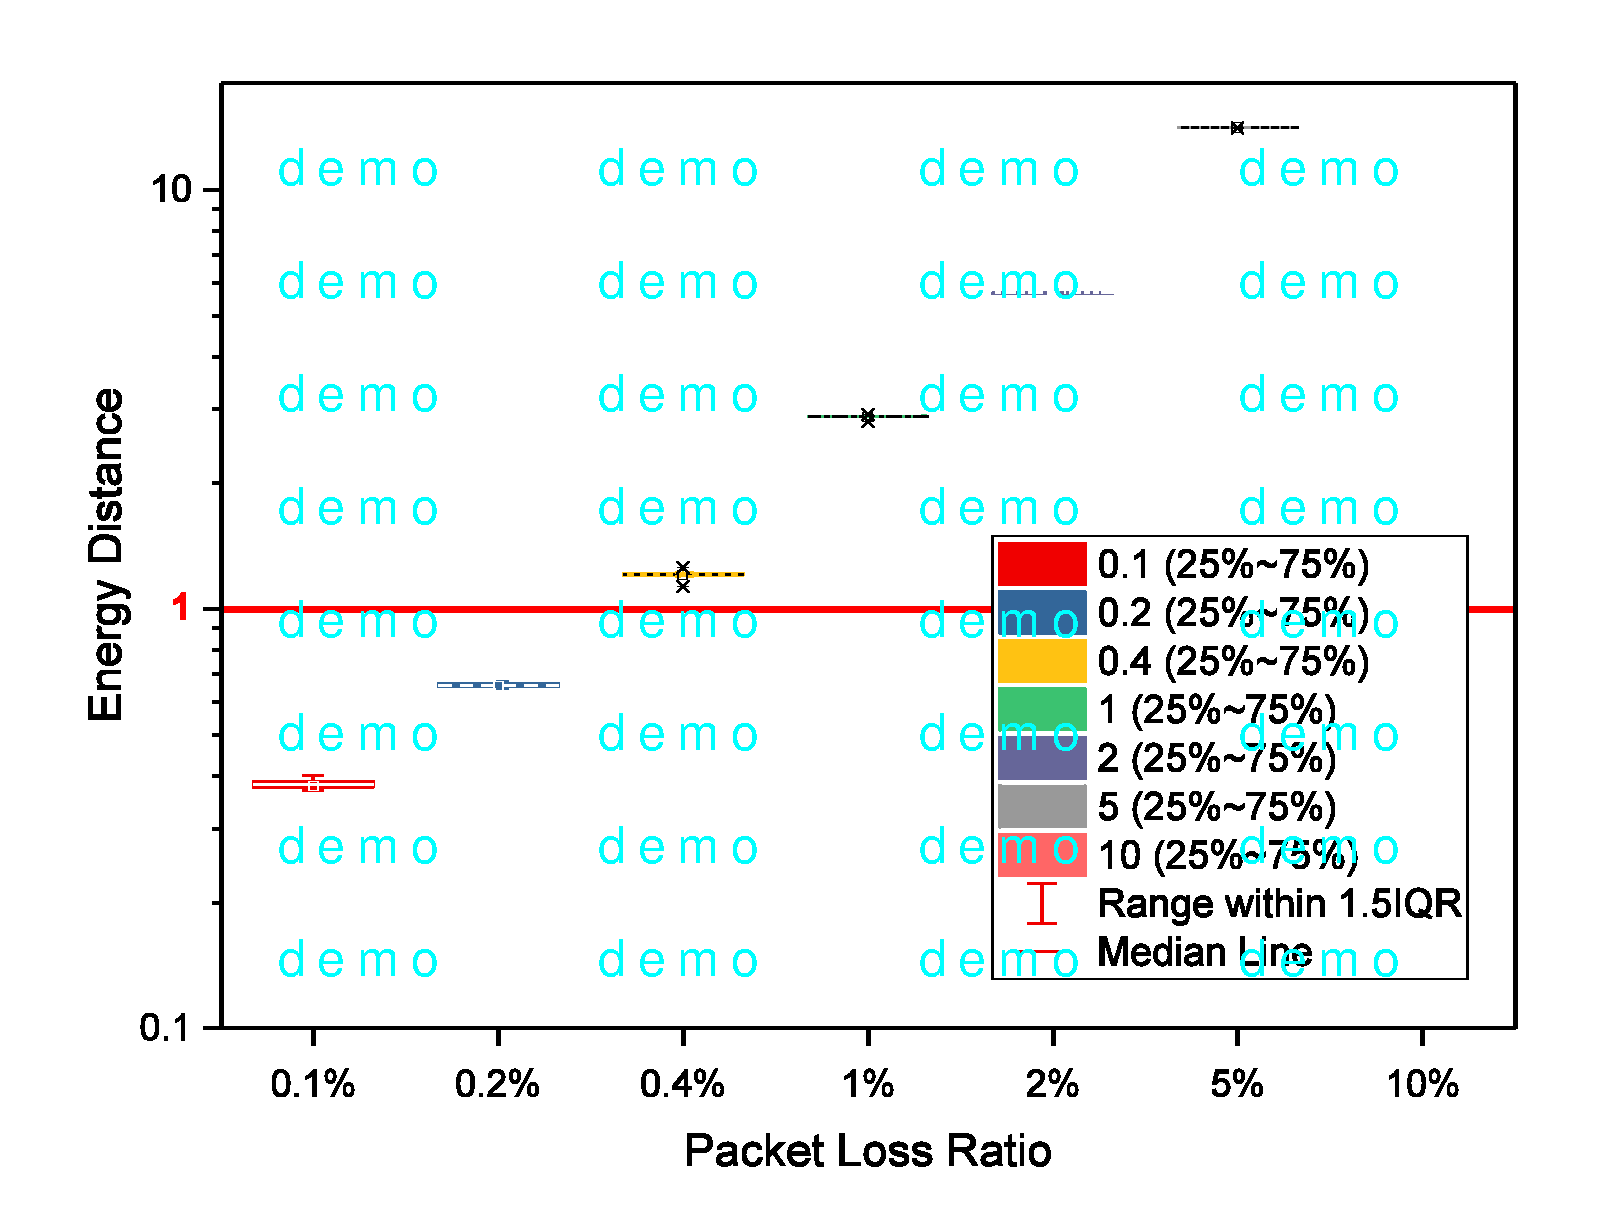
\includegraphics[width=0.48\textwidth]{chapters/chapter3/figures/win200-ed-excellent.pdf}
        }
        \subfigure[窗口200时Good场景能量距离的箱线图]{
            \label{fig:3:result:win200:ed:good}
            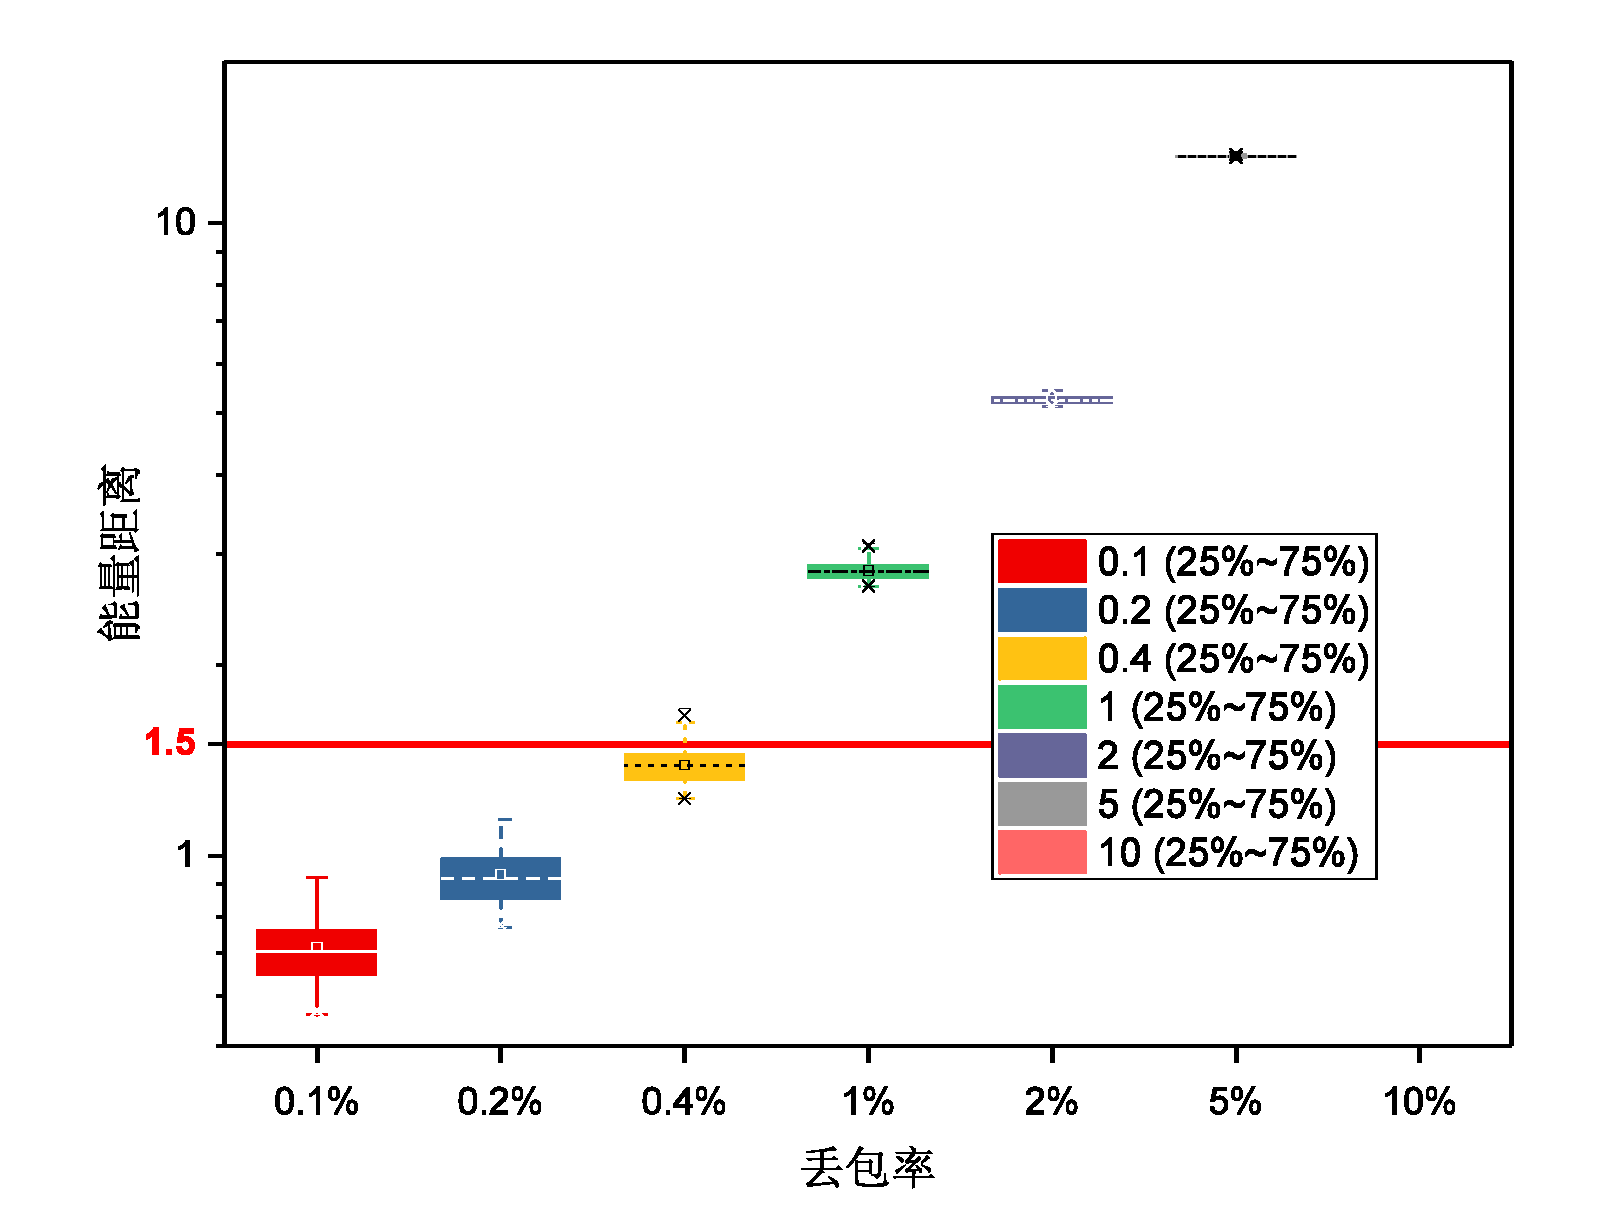
\includegraphics[width=0.48\textwidth]{chapters/chapter3/figures/win200-ed-good.pdf}
        }
        \caption{区间丢包数能量距离的箱线图}
        \label{fig:3:result:win:ed}
	\end{figure}
}

\subsubsection{CDF测试结果}
\label{chap:analyze:result:window:cdf}

如图\nref{fig:3:result:win:cdf},时间隐通道对CDF曲线产生了显著影响。对比图\nref{fig:3:result:win100:cdf:excellent}及图\nref{fig:3:result:win100:cdf:good},在相同的窗口设置下,由于不同场景中的丢包情况不同,Excellent场景下的CDF曲线上升趋势更加明显,也就意味着丢包数较多的区间占据的比例较低。对比图\nref{fig:3:result:win100:cdf:excellent}及图\nref{fig:3:result:win200:cdf:excellent},在相同场景中,增大窗口长度后,曲线的上升趋势减缓,更有利于判断分布的差异。

通过对比CDF曲线,可以明显发现时间隐通道的丢包越密集,对曲线的影响越大。当丢包的间隔小于区间长度时,意味着区间内一定存在丢包的情况,导致CDF曲线的起始位置大于0,出现明显的异常现象。因此,通过CDF曲线可以发现丢包率$\ge5\%$的时间隐通道。

\subsubsection{条件熵测试结果}
\label{chap:analyze:result:window:kld}

K-L散度的测试结果如图\nref{fig:3:result:win:kld},两种场景下,两种窗口长度的分布均通过了K-L散度检验。考虑到K-L散度的计算方式如公式(\nref{equ:2:kld}),对$f(x)$及$g(x)$有$f(x)>0$及$g(x)>0$的约束,相当于CDF曲线起点统一对齐到$(0,0)$点。而图\nref{fig:3:result:win:cdf}中各曲线的趋势是相同的,也就意味着概率分布函数在非零处基本一致,导致K-L散度检测无法有效区分。

\subsubsection{相对距离测试结果}
\label{chap:analyze:result:window:distance}

Wasserstein距离的检测结果如图\nref{fig:3:result:win:wd}。可以发现,计算得到的Wasserstein距离,能够有效区分不同丢包率下时间隐通道产生的影响。当窗口长度为100时,只有丢包率$\le 1\%$才可以通过Wasserstein距离检验;而窗口长度扩展到200时,只有丢包率$\le 0.4\%$才可以通过检测。

能量距离的检测结果如图\nref{fig:3:result:win:ed}。检测结果类似于Wasserstein距离检测,在窗口长度为100时,只有丢包率$\le 1\%$才可以通过测试;而在窗口长度为200时,需要丢包率$\le 0.4\%$才有较高的通过几率。

通过检测结果可以发现,能量距离可以很好地反映CDF曲线的差异,与K-L散度相结合,可以从不同的方面对分布之间的差异进行评估。实验结果证明,通过结合区间丢包数分布和突发丢包长度,可以对基于IPD的检测方法进行补充。


%\subsection{无参考视频质量评价}
%\label{chap:analyze:result:burst:vqm}

%计算PSNR等无参考视频质量结果,说明两种场景下,应当满足的视频质量

%NIQE(Natural Image Quality Evaluator)\nupcite{6353522}

\subsection{检测结果汇总}
根据表\nref{tab:3:detect-sum}中设定的14种测试项,根据其中的11条量化评估条目,生成了该检测方法结果的汇总表。

\insertTable{
	\begin{table}[]
      \centering
      \caption{Excellent场景下时间隐通道检出率汇总表}
      \label{tab:3:result-sum:excellent}
          \begin{tabular*}{0.99\textwidth}{@{\extracolsep{\fill}}ccccccccc}
            \toprule
            对象 & 方法 & 10\% & 5\% & 2\% & 1\% & 0.4\% & 0.2\% & 0.1\%\\ 
            \midrule
            \multirow{5}{*}{IPD分布} & K-S检验 & 100\% & 100\% & 100\% & 0\% & 0\% & 0\% & 0\% \\
            & t检验,rank检验 & 100\% & 100\% & 100\% & 100\% & 0\% & 0\% & 0\% \\
            & K-L散度 & 0\% & 0\% & 0\% & 0\% & 0\% & 0\% & 0\% \\
            & Wasserstein距离 & 0\% & 0\% & 0\% & 0\% & 0\% & 0\% & 0\% \\
            & 能量距离 & 100\% & 0\% & 0\% & 0\% & 0\% & 0\% & 0\% \\
            \\
            \multirow{3}{*}{突发丢包长度} & K-L散度 & 100\% & 100\% & 100\% & 100\% & 100\% & 0\% & 0\% \\
            & Wasserstein距离 & 0\% & 0\% & 0\% & 0\% & 0\% & 0\% & 0\% \\
            & 能量距离 & 100\% & 100\% & 0\% & 0\% & 0\% & 0\% & 0\% \\
            \\
            \multirow{3}{*}{区间丢包数} & K-L散度 & 0\% & 0\% & 0\% & 0\% & 0\% & 0\% & 0\% \\
            & Wasserstein距离 & 100\% & 100\% & 100\% & 100\% & 0\% & 0\% & 0\% \\
            & 能量距离 & 100\% & 100\% & 100\% & 100\% & 0\% & 0\% & 0\% \\
            \bottomrule
          \end{tabular*}
    \end{table}
}

\insertTable{
	\begin{table}[]
      \centering
      \caption{Good场景下时间隐通道检出率汇总表}
      \label{tab:3:result-sum:good}
          \begin{tabular*}{0.99\textwidth}{@{\extracolsep{\fill}}ccccccccc}
            \toprule
            对象 & 方法 & 10\% & 5\% & 2\% & 1\% & 0.4\% & 0.2\% & 0.1\%\\ 
            \midrule
            \multirow{5}{*}{IPD分布} & K-S检验 & 100\% & 100\% & 100\% & 0\% & 0\% & 0\% & 0\% \\
            & t检验,rank检验 & 100\% & 100\% & 0\% & 0\% & 0\% & 0\% & 0\% \\
            & K-L散度 & 0\% & 0\% & 0\% & 0\% & 0\% & 0\% & 0\% \\
            & Wasserstein距离 & 0\% & 0\% & 0\% & 0\% & 0\% & 0\% & 0\% \\
            & 能量距离 & 100\% & 0\% & 0\% & 0\% & 0\% & 0\% & 0\% \\
            \\
            \multirow{3}{*}{突发丢包长度} & K-L散度 & 100\% & 100\% & 100\% & 0\% & 0\% & 0\% & 0\% \\
            & Wasserstein距离 & 100\% & 100\% & 0\% & 0\% & 0\% & 0\% & 0\% \\
            & 能量距离 & 100\% & 100\% & 100\% & 0\% & 0\% & 0\% & 0\% \\
            \\
            \multirow{3}{*}{区间丢包数} & K-L散度 & 0\% & 0\% & 0\% & 0\% & 0\% & 0\% & 0\% \\
            & Wasserstein距离 & 100\% & 100\% & 100\% & 100\% & 11\% & 0\% & 0\% \\
            & 能量距离 & 100\% & 100\% & 100\% & 100\% & 11\% & 0\% & 0\% \\
            \bottomrule
          \end{tabular*}
    \end{table}
}

如表\nref{tab:3:result-sum:excellent}及表\nref{tab:3:result-sum:good},不同方法的检出率存在显著区别,在不同场景下的相同方法也存在明显差距。在Excellent场景中,基于IPD的检测方法检出能力较弱,而突发长度的检测及区间丢包数的检测,具有很均衡的检测效果,可以准确检测出主动丢包产生的影响。当主动丢包的密度降低到一定程度,超过检测方法的敏感度,便无法检测出时间隐通道的存在。

在Good场景中,基于IPD的检测方法同样具有较弱的检测能力。由于信道中已经存在一定比例的丢包事件,基于突发长度的检测方法分辨能力减弱;但基于区间丢包数的检测方法,能够进一步区分出长度为1的随机丢包,因此具有较好的检测效果。

\insertTable{
	\begin{table}[]
      \centering
      \caption{时间隐通道检出率汇总表}
      \label{tab:3:result-sum:all}
          \begin{tabular*}{0.99\textwidth}{@{\extracolsep{\fill}}cccccccc}
            \toprule
            场景 & 10\% & 5\% & 2\% & 1\% & 0.4\% & 0.2\% & 0.1\% \\ 
            \midrule
            Excellent & 100\% & 100\% & 100\% & 100\% & 100\% & 0\% & 0\% \\
            Good & 100\% & 100\% & 100\% & 100\% & 11\% & 0\% & 0\% \\
            \bottomrule
          \end{tabular*}
    \end{table}
}

在不同场景下,该检测方法,对不同丢包比例的时间隐通道检测能力如表\nref{tab:3:result-sum:all}。由表可知,该检测方法对统计分布变化非常敏感,只有时间隐通道产生的丢包控制在$0.1\%\sim0.4\%$左右,才有可能通过检测。